\documentclass[twoside]{book}

% Packages required by doxygen
\usepackage{fixltx2e}
\usepackage{calc}
\usepackage{doxygen}
\usepackage{graphicx}
\usepackage[utf8]{inputenc}
\usepackage{makeidx}
\usepackage{multicol}
\usepackage{multirow}
\PassOptionsToPackage{warn}{textcomp}
\usepackage{textcomp}
\usepackage[nointegrals]{wasysym}
\usepackage[table]{xcolor}

% Font selection
\usepackage[T1]{fontenc}
\usepackage{mathptmx}
\usepackage[scaled=.90]{helvet}
\usepackage{courier}
\usepackage{amssymb}
\usepackage{sectsty}
\renewcommand{\familydefault}{\sfdefault}
\allsectionsfont{%
  \fontseries{bc}\selectfont%
  \color{darkgray}%
}
\renewcommand{\DoxyLabelFont}{%
  \fontseries{bc}\selectfont%
  \color{darkgray}%
}
\newcommand{\+}{\discretionary{\mbox{\scriptsize$\hookleftarrow$}}{}{}}

% Page & text layout
\usepackage{geometry}
\geometry{%
  a4paper,%
  top=2.5cm,%
  bottom=2.5cm,%
  left=2.5cm,%
  right=2.5cm%
}
\tolerance=750
\hfuzz=15pt
\hbadness=750
\setlength{\emergencystretch}{15pt}
\setlength{\parindent}{0cm}
\setlength{\parskip}{0.2cm}
\makeatletter
\renewcommand{\paragraph}{%
  \@startsection{paragraph}{4}{0ex}{-1.0ex}{1.0ex}{%
    \normalfont\normalsize\bfseries\SS@parafont%
  }%
}
\renewcommand{\subparagraph}{%
  \@startsection{subparagraph}{5}{0ex}{-1.0ex}{1.0ex}{%
    \normalfont\normalsize\bfseries\SS@subparafont%
  }%
}
\makeatother

% Headers & footers
\usepackage{fancyhdr}
\pagestyle{fancyplain}
\fancyhead[LE]{\fancyplain{}{\bfseries\thepage}}
\fancyhead[CE]{\fancyplain{}{}}
\fancyhead[RE]{\fancyplain{}{\bfseries\leftmark}}
\fancyhead[LO]{\fancyplain{}{\bfseries\rightmark}}
\fancyhead[CO]{\fancyplain{}{}}
\fancyhead[RO]{\fancyplain{}{\bfseries\thepage}}
\fancyfoot[LE]{\fancyplain{}{}}
\fancyfoot[CE]{\fancyplain{}{}}
\fancyfoot[RE]{\fancyplain{}{\bfseries\scriptsize Generated on Wed Dec 7 2016 09\+:11\+:03 for My Project by Doxygen }}
\fancyfoot[LO]{\fancyplain{}{\bfseries\scriptsize Generated on Wed Dec 7 2016 09\+:11\+:03 for My Project by Doxygen }}
\fancyfoot[CO]{\fancyplain{}{}}
\fancyfoot[RO]{\fancyplain{}{}}
\renewcommand{\footrulewidth}{0.4pt}
\renewcommand{\chaptermark}[1]{%
  \markboth{#1}{}%
}
\renewcommand{\sectionmark}[1]{%
  \markright{\thesection\ #1}%
}

% Indices & bibliography
\usepackage{natbib}
\usepackage[titles]{tocloft}
\setcounter{tocdepth}{3}
\setcounter{secnumdepth}{5}
\makeindex

% Hyperlinks (required, but should be loaded last)
\usepackage{ifpdf}
\ifpdf
  \usepackage[pdftex,pagebackref=true]{hyperref}
\else
  \usepackage[ps2pdf,pagebackref=true]{hyperref}
\fi
\hypersetup{%
  colorlinks=true,%
  linkcolor=blue,%
  citecolor=blue,%
  unicode%
}

% Custom commands
\newcommand{\clearemptydoublepage}{%
  \newpage{\pagestyle{empty}\cleardoublepage}%
}


%===== C O N T E N T S =====

\begin{document}

% Titlepage & ToC
\hypersetup{pageanchor=false,
             bookmarks=true,
             bookmarksnumbered=true,
             pdfencoding=unicode
            }
\pagenumbering{roman}
\begin{titlepage}
\vspace*{7cm}
\begin{center}%
{\Large My Project }\\
\vspace*{1cm}
{\large Generated by Doxygen 1.8.7}\\
\vspace*{0.5cm}
{\small Wed Dec 7 2016 09:11:03}\\
\end{center}
\end{titlepage}
\clearemptydoublepage
\tableofcontents
\clearemptydoublepage
\pagenumbering{arabic}
\hypersetup{pageanchor=true}

%--- Begin generated contents ---
\chapter{Projet\+C}
\label{md_README}
\hypertarget{md_README}{}
\input{md_README}
\chapter{Hierarchical Index}
\section{Class Hierarchy}
This inheritance list is sorted roughly, but not completely, alphabetically\+:\begin{DoxyCompactList}
\item \contentsline{section}{Affichage\+Init}{\pageref{class_affichage_init}}{}
\begin{DoxyCompactList}
\item \contentsline{section}{Affichage\+Init\+J1}{\pageref{class_affichage_init_j1}}{}
\item \contentsline{section}{Affichage\+Init\+J2}{\pageref{class_affichage_init_j2}}{}
\end{DoxyCompactList}
\item \contentsline{section}{Bateau\+Factory}{\pageref{class_bateau_factory}}{}
\begin{DoxyCompactList}
\item \contentsline{section}{Factory\+Canard}{\pageref{class_factory_canard}}{}
\item \contentsline{section}{Factory\+Caneton}{\pageref{class_factory_caneton}}{}
\item \contentsline{section}{Factory\+Cygne}{\pageref{class_factory_cygne}}{}
\item \contentsline{section}{Factory\+Oie}{\pageref{class_factory_oie}}{}
\end{DoxyCompactList}
\item \contentsline{section}{Comp\+Mode}{\pageref{class_comp_mode}}{}
\begin{DoxyCompactList}
\item \contentsline{section}{Mode1vs1}{\pageref{class_mode1vs1}}{}
\item \contentsline{section}{Mode1vs\+IA}{\pageref{class_mode1vs_i_a}}{}
\end{DoxyCompactList}
\item \contentsline{section}{Contenu}{\pageref{class_contenu}}{}
\begin{DoxyCompactList}
\item \contentsline{section}{Bateau}{\pageref{class_bateau}}{}
\begin{DoxyCompactList}
\item \contentsline{section}{Canard}{\pageref{class_canard}}{}
\item \contentsline{section}{Caneton}{\pageref{class_caneton}}{}
\item \contentsline{section}{Cygne}{\pageref{class_cygne}}{}
\item \contentsline{section}{Oie}{\pageref{class_oie}}{}
\end{DoxyCompactList}
\item \contentsline{section}{Mer}{\pageref{class_mer}}{}
\end{DoxyCompactList}
\item \contentsline{section}{Core}{\pageref{class_core}}{}
\item Q\+Push\+Button\begin{DoxyCompactList}
\item \contentsline{section}{Case}{\pageref{class_case}}{}
\end{DoxyCompactList}
\item Q\+Widget\begin{DoxyCompactList}
\item \contentsline{section}{Carte}{\pageref{class_carte}}{}
\begin{DoxyCompactList}
\item \contentsline{section}{Carte\+Init}{\pageref{class_carte_init}}{}
\item \contentsline{section}{Carte\+Jeu}{\pageref{class_carte_jeu}}{}
\end{DoxyCompactList}
\item \contentsline{section}{I\+Affichage}{\pageref{class_i_affichage}}{}
\begin{DoxyCompactList}
\item \contentsline{section}{Affichage\+Init\+J1}{\pageref{class_affichage_init_j1}}{}
\item \contentsline{section}{Affichage\+Init\+J2}{\pageref{class_affichage_init_j2}}{}
\item \contentsline{section}{Affichage\+Jeu}{\pageref{class_affichage_jeu}}{}
\item \contentsline{section}{Affichage\+Menu}{\pageref{class_affichage_menu}}{}
\end{DoxyCompactList}
\end{DoxyCompactList}
\item \contentsline{section}{Team}{\pageref{class_team}}{}
\end{DoxyCompactList}

\chapter{Class Index}
\section{Class List}
Here are the classes, structs, unions and interfaces with brief descriptions\+:\begin{DoxyCompactList}
\item\contentsline{section}{\hyperlink{class_affichage_init}{Affichage\+Init} \\*Classe representant l\textquotesingle{}affichage des éléments communs pour l\textquotesingle{}initialisation des deux joueurs }{\pageref{class_affichage_init}}{}
\item\contentsline{section}{\hyperlink{class_affichage_init_j1}{Affichage\+Init\+J1} \\*Classe representant l\textquotesingle{}affichage de la phase d\textquotesingle{}initialisation du J1 }{\pageref{class_affichage_init_j1}}{}
\item\contentsline{section}{\hyperlink{class_affichage_init_j2}{Affichage\+Init\+J2} \\*Classe representant l\textquotesingle{}affichage de la phase d\textquotesingle{}initialisation du J2 }{\pageref{class_affichage_init_j2}}{}
\item\contentsline{section}{\hyperlink{class_affichage_jeu}{Affichage\+Jeu} \\*Classe representant l\textquotesingle{}affichage du jeu }{\pageref{class_affichage_jeu}}{}
\item\contentsline{section}{\hyperlink{class_affichage_menu}{Affichage\+Menu} \\*Classe representant l\textquotesingle{}affichage du menu }{\pageref{class_affichage_menu}}{}
\item\contentsline{section}{\hyperlink{class_bateau}{Bateau} \\*Classe representant un \hyperlink{class_bateau}{Bateau} }{\pageref{class_bateau}}{}
\item\contentsline{section}{\hyperlink{class_bateau_factory}{Bateau\+Factory} \\*Classe representant un \char`\"{}\+Chantier Naval\char`\"{} }{\pageref{class_bateau_factory}}{}
\item\contentsline{section}{\hyperlink{class_canard}{Canard} \\*Classe representant un \hyperlink{class_canard}{Canard} }{\pageref{class_canard}}{}
\item\contentsline{section}{\hyperlink{class_caneton}{Caneton} \\*Classe representant un \hyperlink{class_caneton}{Caneton} }{\pageref{class_caneton}}{}
\item\contentsline{section}{\hyperlink{class_carte}{Carte} \\*Classe representant une \hyperlink{class_carte}{Carte} }{\pageref{class_carte}}{}
\item\contentsline{section}{\hyperlink{class_carte_init}{Carte\+Init} \\*Classe representant une \hyperlink{class_carte}{Carte} d\textquotesingle{}initialisation }{\pageref{class_carte_init}}{}
\item\contentsline{section}{\hyperlink{class_carte_jeu}{Carte\+Jeu} \\*Classe representant une \hyperlink{class_carte}{Carte} de jeu }{\pageref{class_carte_jeu}}{}
\item\contentsline{section}{\hyperlink{class_case}{Case} \\*Classe representant une \hyperlink{class_case}{Case} }{\pageref{class_case}}{}
\item\contentsline{section}{\hyperlink{class_comp_mode}{Comp\+Mode} \\*Classe representant un comportement de mode de jeu }{\pageref{class_comp_mode}}{}
\item\contentsline{section}{\hyperlink{class_contenu}{Contenu} \\*Classe representant un \hyperlink{class_contenu}{Contenu} }{\pageref{class_contenu}}{}
\item\contentsline{section}{\hyperlink{class_core}{Core} }{\pageref{class_core}}{}
\item\contentsline{section}{\hyperlink{class_cygne}{Cygne} \\*Classe representant un \hyperlink{class_cygne}{Cygne} }{\pageref{class_cygne}}{}
\item\contentsline{section}{\hyperlink{class_factory_canard}{Factory\+Canard} \\*Classe representant une usine à \hyperlink{class_canard}{Canard} }{\pageref{class_factory_canard}}{}
\item\contentsline{section}{\hyperlink{class_factory_caneton}{Factory\+Caneton} \\*Classe representant une usine à \hyperlink{class_caneton}{Caneton} }{\pageref{class_factory_caneton}}{}
\item\contentsline{section}{\hyperlink{class_factory_cygne}{Factory\+Cygne} \\*Classe representant une usine à \hyperlink{class_cygne}{Cygne} }{\pageref{class_factory_cygne}}{}
\item\contentsline{section}{\hyperlink{class_factory_oie}{Factory\+Oie} \\*Classe representant une usine à \hyperlink{class_oie}{Oie} }{\pageref{class_factory_oie}}{}
\item\contentsline{section}{\hyperlink{class_i_affichage}{I\+Affichage} \\*Classe representant les comportements des affichages }{\pageref{class_i_affichage}}{}
\item\contentsline{section}{\hyperlink{class_mer}{Mer} \\*Classe representant de la \hyperlink{class_mer}{Mer} }{\pageref{class_mer}}{}
\item\contentsline{section}{\hyperlink{class_mode1vs1}{Mode1vs1} \\*Classe representant le mode de jeu 1\+V\+S1 }{\pageref{class_mode1vs1}}{}
\item\contentsline{section}{\hyperlink{class_mode1vs_i_a}{Mode1vs\+IA} \\*Classe representant le mode de jeu 1\+V\+S\+IA }{\pageref{class_mode1vs_i_a}}{}
\item\contentsline{section}{\hyperlink{class_oie}{Oie} \\*Classe representant un \hyperlink{class_oie}{Oie} }{\pageref{class_oie}}{}
\item\contentsline{section}{\hyperlink{class_team}{Team} \\*Classe representant un Joueur }{\pageref{class_team}}{}
\end{DoxyCompactList}

\chapter{Class Documentation}
\hypertarget{classAffichageInit}{\section{Affichage\+Init Class Reference}
\label{classAffichageInit}\index{Affichage\+Init@{Affichage\+Init}}
}


classe representant l'affichage des éléments communs pour l'initialisation des deux joueurs  




{\ttfamily \#include $<$affichageinit.\+h$>$}



Inheritance diagram for Affichage\+Init\+:
\nopagebreak
\begin{figure}[H]
\begin{center}
\leavevmode
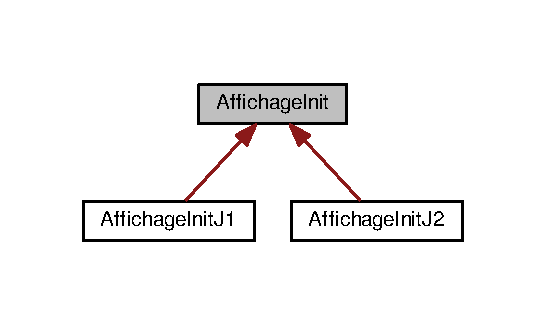
\includegraphics[width=262pt]{classAffichageInit__inherit__graph}
\end{center}
\end{figure}
\subsection*{Public Member Functions}
\begin{DoxyCompactItemize}
\item 
\hypertarget{classAffichageInit_a5edfda4c52c2c15fbb9ee87112deebe4}{\hyperlink{classAffichageInit_a5edfda4c52c2c15fbb9ee87112deebe4}{Affichage\+Init} ()}\label{classAffichageInit_a5edfda4c52c2c15fbb9ee87112deebe4}

\begin{DoxyCompactList}\small\item\em Constructeur Constructeur de la classe \hyperlink{classAffichageInit}{Affichage\+Init}. \end{DoxyCompactList}\item 
void \hyperlink{classAffichageInit_ad8af1158fc6b73fa42817d3f610a82c5}{update\+Elements} (std\+::string txt\+Bt)
\begin{DoxyCompactList}\small\item\em Ajout de tous les éléments pour l'affichage. \end{DoxyCompactList}\item 
bool \hyperlink{classAffichageInit_a2cc64639534b8088912c64d733937508}{h\+Checked} ()
\begin{DoxyCompactList}\small\item\em \hyperlink{classCase}{Case} pour bateau horizontal cochée ? \end{DoxyCompactList}\item 
Q\+Radio\+Button $\ast$ \hyperlink{classAffichageInit_a5c268472841e36e713ea27c1675c6e11}{get\+B4} ()
\begin{DoxyCompactList}\small\item\em Retourne le radiobouton cliqué \end{DoxyCompactList}\item 
Q\+Radio\+Button $\ast$ \hyperlink{classAffichageInit_acb11d9f4409fabf79a63b0a3362ffdbb}{get\+B3} ()
\begin{DoxyCompactList}\small\item\em Retourne le radiobouton cliqué \end{DoxyCompactList}\item 
Q\+Radio\+Button $\ast$ \hyperlink{classAffichageInit_a6f5a1714feffff2e93cb7d80509576ff}{get\+B2} ()
\begin{DoxyCompactList}\small\item\em Retourne le radiobouton cliqué \end{DoxyCompactList}\item 
Q\+Radio\+Button $\ast$ \hyperlink{classAffichageInit_a79cbb21d4b8b84ad87f13ec7f7fb5224}{get\+B1} ()
\begin{DoxyCompactList}\small\item\em Retourne le radiobouton cliqué \end{DoxyCompactList}\item 
Q\+Radio\+Button $\ast$ \hyperlink{classAffichageInit_a9334010a1147906ffd45dbb48a63ad6e}{get\+Bateau\+Select} ()
\begin{DoxyCompactList}\small\item\em Retourne le radiobouton cliqué \end{DoxyCompactList}\item 
void \hyperlink{classAffichageInit_a55b47fb580a1eb29aa79475453c6936b}{reset\+Bouton} ()
\begin{DoxyCompactList}\small\item\em Permet de remettre à zéro la carte. \end{DoxyCompactList}\end{DoxyCompactItemize}
\subsection*{Protected Attributes}
\begin{DoxyCompactItemize}
\item 
Q\+Grid\+Layout $\ast$ \hyperlink{classAffichageInit_a6cfa8eefd38ed8397269da4b472d7ad5}{g\+Layout\+Central\+\_\+}
\item 
Q\+Grid\+Layout $\ast$ \hyperlink{classAffichageInit_a7e46084cc3c86b029ac04b59f3e70d5e}{g\+Layout\+Gauche\+\_\+}
\item 
Q\+Grid\+Layout $\ast$ \hyperlink{classAffichageInit_a30c6eb873576eb8c416091b3fe54d46a}{g\+Layout\+Droite\+\_\+}
\item 
std\+::shared\+\_\+ptr$<$ \hyperlink{classCarte}{Carte} $>$ \hyperlink{classAffichageInit_ae64aeadaa88e3d7b62c9b8edb77f4bc1}{carte\+Init\+\_\+}
\item 
Q\+Radio\+Button $\ast$ \hyperlink{classAffichageInit_a705aa3459121ac5b4ef60520fb0b509f}{b1\+\_\+}
\item 
Q\+Radio\+Button $\ast$ \hyperlink{classAffichageInit_ac8c97eaabcc52302156b5d0fb2dd4b7f}{b2\+\_\+}
\item 
Q\+Radio\+Button $\ast$ \hyperlink{classAffichageInit_afc2ce79e46033da8e7949f69fee1811c}{b3\+\_\+}
\item 
Q\+Radio\+Button $\ast$ \hyperlink{classAffichageInit_a364a79854751059ea883f4f111416e27}{b4\+\_\+}
\item 
Q\+Line\+Edit $\ast$ \hyperlink{classAffichageInit_a5327093a0df1060ada2be6678a3d2c2e}{pseudo\+\_\+}
\item 
Q\+Check\+Box $\ast$ \hyperlink{classAffichageInit_ad3535a45425dc7a11b8f0ed8c4b07f4c}{horizontal\+\_\+}
\item 
Q\+Push\+Button $\ast$ \hyperlink{classAffichageInit_a2d5808b5c427d934c16b6ffb1046ea1a}{bouton\+Suivant\+\_\+}
\item 
Q\+Push\+Button $\ast$ \hyperlink{classAffichageInit_a057a07eb4c76bde07bf75eb0d7a45f73}{reset\+\_\+}
\end{DoxyCompactItemize}


\subsection{Detailed Description}
classe representant l'affichage des éléments communs pour l'initialisation des deux joueurs 

La classe gère l'affichage de l'ensemble des éléments qu'auront besoin les joueurs pour la phase d'initialisation 

\subsection{Member Function Documentation}
\hypertarget{classAffichageInit_a79cbb21d4b8b84ad87f13ec7f7fb5224}{\index{Affichage\+Init@{Affichage\+Init}!get\+B1@{get\+B1}}
\index{get\+B1@{get\+B1}!Affichage\+Init@{Affichage\+Init}}
\subsubsection[{get\+B1}]{\setlength{\rightskip}{0pt plus 5cm}Q\+Radio\+Button $\ast$ Affichage\+Init\+::get\+B1 (
\begin{DoxyParamCaption}
{}
\end{DoxyParamCaption}
)}}\label{classAffichageInit_a79cbb21d4b8b84ad87f13ec7f7fb5224}


Retourne le radiobouton cliqué 

Methode qui permet de retourner si le bouton représentant le bateau de taille 1 est cliqué

\begin{DoxyReturn}{Returns}
le bouton sur lequel on a cliqué 
\end{DoxyReturn}
\hypertarget{classAffichageInit_a6f5a1714feffff2e93cb7d80509576ff}{\index{Affichage\+Init@{Affichage\+Init}!get\+B2@{get\+B2}}
\index{get\+B2@{get\+B2}!Affichage\+Init@{Affichage\+Init}}
\subsubsection[{get\+B2}]{\setlength{\rightskip}{0pt plus 5cm}Q\+Radio\+Button $\ast$ Affichage\+Init\+::get\+B2 (
\begin{DoxyParamCaption}
{}
\end{DoxyParamCaption}
)}}\label{classAffichageInit_a6f5a1714feffff2e93cb7d80509576ff}


Retourne le radiobouton cliqué 

Methode qui permet de retourner si le bouton représentant le bateau de taille 2 est cliqué

\begin{DoxyReturn}{Returns}
le bouton sur lequel on a cliqué 
\end{DoxyReturn}
\hypertarget{classAffichageInit_acb11d9f4409fabf79a63b0a3362ffdbb}{\index{Affichage\+Init@{Affichage\+Init}!get\+B3@{get\+B3}}
\index{get\+B3@{get\+B3}!Affichage\+Init@{Affichage\+Init}}
\subsubsection[{get\+B3}]{\setlength{\rightskip}{0pt plus 5cm}Q\+Radio\+Button $\ast$ Affichage\+Init\+::get\+B3 (
\begin{DoxyParamCaption}
{}
\end{DoxyParamCaption}
)}}\label{classAffichageInit_acb11d9f4409fabf79a63b0a3362ffdbb}


Retourne le radiobouton cliqué 

Methode qui permet de retourner si le bouton représentant le bateau de taille 3 est cliqué

\begin{DoxyReturn}{Returns}
le bouton sur lequel on a cliqué 
\end{DoxyReturn}
\hypertarget{classAffichageInit_a5c268472841e36e713ea27c1675c6e11}{\index{Affichage\+Init@{Affichage\+Init}!get\+B4@{get\+B4}}
\index{get\+B4@{get\+B4}!Affichage\+Init@{Affichage\+Init}}
\subsubsection[{get\+B4}]{\setlength{\rightskip}{0pt plus 5cm}Q\+Radio\+Button $\ast$ Affichage\+Init\+::get\+B4 (
\begin{DoxyParamCaption}
{}
\end{DoxyParamCaption}
)}}\label{classAffichageInit_a5c268472841e36e713ea27c1675c6e11}


Retourne le radiobouton cliqué 

Methode qui permet de retourner si le bouton représentant le bateau de taille 4 est cliqué

\begin{DoxyReturn}{Returns}
le bouton sur lequel on a cliqué 
\end{DoxyReturn}
\hypertarget{classAffichageInit_a9334010a1147906ffd45dbb48a63ad6e}{\index{Affichage\+Init@{Affichage\+Init}!get\+Bateau\+Select@{get\+Bateau\+Select}}
\index{get\+Bateau\+Select@{get\+Bateau\+Select}!Affichage\+Init@{Affichage\+Init}}
\subsubsection[{get\+Bateau\+Select}]{\setlength{\rightskip}{0pt plus 5cm}Q\+Radio\+Button $\ast$ Affichage\+Init\+::get\+Bateau\+Select (
\begin{DoxyParamCaption}
{}
\end{DoxyParamCaption}
)}}\label{classAffichageInit_a9334010a1147906ffd45dbb48a63ad6e}


Retourne le radiobouton cliqué 

Methode qui permet de retourner directement sur quel radiobouton, concernant les bateaux, on a cliqué

\begin{DoxyReturn}{Returns}
le bouton sur lequel on a cliqué 
\end{DoxyReturn}
\hypertarget{classAffichageInit_a2cc64639534b8088912c64d733937508}{\index{Affichage\+Init@{Affichage\+Init}!h\+Checked@{h\+Checked}}
\index{h\+Checked@{h\+Checked}!Affichage\+Init@{Affichage\+Init}}
\subsubsection[{h\+Checked}]{\setlength{\rightskip}{0pt plus 5cm}bool Affichage\+Init\+::h\+Checked (
\begin{DoxyParamCaption}
{}
\end{DoxyParamCaption}
)}}\label{classAffichageInit_a2cc64639534b8088912c64d733937508}


\hyperlink{classCase}{Case} pour bateau horizontal cochée ? 

Methode qui permet de tester si la case, pour savoir si le bateau que l'on veut placer sera horizontal, est cochée

\begin{DoxyReturn}{Returns}
true si le bateau sera horizontal, false sinon 
\end{DoxyReturn}
\hypertarget{classAffichageInit_a55b47fb580a1eb29aa79475453c6936b}{\index{Affichage\+Init@{Affichage\+Init}!reset\+Bouton@{reset\+Bouton}}
\index{reset\+Bouton@{reset\+Bouton}!Affichage\+Init@{Affichage\+Init}}
\subsubsection[{reset\+Bouton}]{\setlength{\rightskip}{0pt plus 5cm}void Affichage\+Init\+::reset\+Bouton (
\begin{DoxyParamCaption}
{}
\end{DoxyParamCaption}
)}}\label{classAffichageInit_a55b47fb580a1eb29aa79475453c6936b}


Permet de remettre à zéro la carte. 

Methode qui permet de reset l'ensemble des bateaux présent sur la carte \hypertarget{classAffichageInit_ad8af1158fc6b73fa42817d3f610a82c5}{\index{Affichage\+Init@{Affichage\+Init}!update\+Elements@{update\+Elements}}
\index{update\+Elements@{update\+Elements}!Affichage\+Init@{Affichage\+Init}}
\subsubsection[{update\+Elements}]{\setlength{\rightskip}{0pt plus 5cm}void Affichage\+Init\+::update\+Elements (
\begin{DoxyParamCaption}
\item[{std\+::string}]{txt\+Bt}
\end{DoxyParamCaption}
)}}\label{classAffichageInit_ad8af1158fc6b73fa42817d3f610a82c5}


Ajout de tous les éléments pour l'affichage. 

Methode qui permet d'ajouter l'ensemble des éléments pour l'affichage


\begin{DoxyParams}{Parameters}
{\em txt\+Bt} & \+: le texte sur la bouton \char`\"{}\+Pret\char`\"{} (on indique \char`\"{}suivant\char`\"{}, \char`\"{}jeu\char`\"{}, ...) \\
\hline
\end{DoxyParams}


\subsection{Member Data Documentation}
\hypertarget{classAffichageInit_a705aa3459121ac5b4ef60520fb0b509f}{\index{Affichage\+Init@{Affichage\+Init}!b1\+\_\+@{b1\+\_\+}}
\index{b1\+\_\+@{b1\+\_\+}!Affichage\+Init@{Affichage\+Init}}
\subsubsection[{b1\+\_\+}]{\setlength{\rightskip}{0pt plus 5cm}Q\+Radio\+Button$\ast$ Affichage\+Init\+::b1\+\_\+\hspace{0.3cm}{\ttfamily [protected]}}}\label{classAffichageInit_a705aa3459121ac5b4ef60520fb0b509f}
Bouton pour pouvoir placer les bateaux de taille 1 \hypertarget{classAffichageInit_ac8c97eaabcc52302156b5d0fb2dd4b7f}{\index{Affichage\+Init@{Affichage\+Init}!b2\+\_\+@{b2\+\_\+}}
\index{b2\+\_\+@{b2\+\_\+}!Affichage\+Init@{Affichage\+Init}}
\subsubsection[{b2\+\_\+}]{\setlength{\rightskip}{0pt plus 5cm}Q\+Radio\+Button$\ast$ Affichage\+Init\+::b2\+\_\+\hspace{0.3cm}{\ttfamily [protected]}}}\label{classAffichageInit_ac8c97eaabcc52302156b5d0fb2dd4b7f}
Bouton pour pouvoir placer les bateaux de taille 2 \hypertarget{classAffichageInit_afc2ce79e46033da8e7949f69fee1811c}{\index{Affichage\+Init@{Affichage\+Init}!b3\+\_\+@{b3\+\_\+}}
\index{b3\+\_\+@{b3\+\_\+}!Affichage\+Init@{Affichage\+Init}}
\subsubsection[{b3\+\_\+}]{\setlength{\rightskip}{0pt plus 5cm}Q\+Radio\+Button$\ast$ Affichage\+Init\+::b3\+\_\+\hspace{0.3cm}{\ttfamily [protected]}}}\label{classAffichageInit_afc2ce79e46033da8e7949f69fee1811c}
Bouton pour pouvoir placer les bateaux de taille 3 \hypertarget{classAffichageInit_a364a79854751059ea883f4f111416e27}{\index{Affichage\+Init@{Affichage\+Init}!b4\+\_\+@{b4\+\_\+}}
\index{b4\+\_\+@{b4\+\_\+}!Affichage\+Init@{Affichage\+Init}}
\subsubsection[{b4\+\_\+}]{\setlength{\rightskip}{0pt plus 5cm}Q\+Radio\+Button$\ast$ Affichage\+Init\+::b4\+\_\+\hspace{0.3cm}{\ttfamily [protected]}}}\label{classAffichageInit_a364a79854751059ea883f4f111416e27}
Bouton pour pouvoir placer le bateau de taille 4 \hypertarget{classAffichageInit_a2d5808b5c427d934c16b6ffb1046ea1a}{\index{Affichage\+Init@{Affichage\+Init}!bouton\+Suivant\+\_\+@{bouton\+Suivant\+\_\+}}
\index{bouton\+Suivant\+\_\+@{bouton\+Suivant\+\_\+}!Affichage\+Init@{Affichage\+Init}}
\subsubsection[{bouton\+Suivant\+\_\+}]{\setlength{\rightskip}{0pt plus 5cm}Q\+Push\+Button$\ast$ Affichage\+Init\+::bouton\+Suivant\+\_\+\hspace{0.3cm}{\ttfamily [protected]}}}\label{classAffichageInit_a2d5808b5c427d934c16b6ffb1046ea1a}
Bouton \char`\"{}\+Pret\char`\"{} une fois que tout est O\+K \hypertarget{classAffichageInit_ae64aeadaa88e3d7b62c9b8edb77f4bc1}{\index{Affichage\+Init@{Affichage\+Init}!carte\+Init\+\_\+@{carte\+Init\+\_\+}}
\index{carte\+Init\+\_\+@{carte\+Init\+\_\+}!Affichage\+Init@{Affichage\+Init}}
\subsubsection[{carte\+Init\+\_\+}]{\setlength{\rightskip}{0pt plus 5cm}std\+::shared\+\_\+ptr$<${\bf Carte}$>$ Affichage\+Init\+::carte\+Init\+\_\+\hspace{0.3cm}{\ttfamily [protected]}}}\label{classAffichageInit_ae64aeadaa88e3d7b62c9b8edb77f4bc1}
La carte d'initialisation \hypertarget{classAffichageInit_a6cfa8eefd38ed8397269da4b472d7ad5}{\index{Affichage\+Init@{Affichage\+Init}!g\+Layout\+Central\+\_\+@{g\+Layout\+Central\+\_\+}}
\index{g\+Layout\+Central\+\_\+@{g\+Layout\+Central\+\_\+}!Affichage\+Init@{Affichage\+Init}}
\subsubsection[{g\+Layout\+Central\+\_\+}]{\setlength{\rightskip}{0pt plus 5cm}Q\+Grid\+Layout$\ast$ Affichage\+Init\+::g\+Layout\+Central\+\_\+\hspace{0.3cm}{\ttfamily [protected]}}}\label{classAffichageInit_a6cfa8eefd38ed8397269da4b472d7ad5}
Layout central \hypertarget{classAffichageInit_a30c6eb873576eb8c416091b3fe54d46a}{\index{Affichage\+Init@{Affichage\+Init}!g\+Layout\+Droite\+\_\+@{g\+Layout\+Droite\+\_\+}}
\index{g\+Layout\+Droite\+\_\+@{g\+Layout\+Droite\+\_\+}!Affichage\+Init@{Affichage\+Init}}
\subsubsection[{g\+Layout\+Droite\+\_\+}]{\setlength{\rightskip}{0pt plus 5cm}Q\+Grid\+Layout$\ast$ Affichage\+Init\+::g\+Layout\+Droite\+\_\+\hspace{0.3cm}{\ttfamily [protected]}}}\label{classAffichageInit_a30c6eb873576eb8c416091b3fe54d46a}
Layout contenant les bateaux à placer \hypertarget{classAffichageInit_a7e46084cc3c86b029ac04b59f3e70d5e}{\index{Affichage\+Init@{Affichage\+Init}!g\+Layout\+Gauche\+\_\+@{g\+Layout\+Gauche\+\_\+}}
\index{g\+Layout\+Gauche\+\_\+@{g\+Layout\+Gauche\+\_\+}!Affichage\+Init@{Affichage\+Init}}
\subsubsection[{g\+Layout\+Gauche\+\_\+}]{\setlength{\rightskip}{0pt plus 5cm}Q\+Grid\+Layout$\ast$ Affichage\+Init\+::g\+Layout\+Gauche\+\_\+\hspace{0.3cm}{\ttfamily [protected]}}}\label{classAffichageInit_a7e46084cc3c86b029ac04b59f3e70d5e}
Layout contenant la carte \hypertarget{classAffichageInit_ad3535a45425dc7a11b8f0ed8c4b07f4c}{\index{Affichage\+Init@{Affichage\+Init}!horizontal\+\_\+@{horizontal\+\_\+}}
\index{horizontal\+\_\+@{horizontal\+\_\+}!Affichage\+Init@{Affichage\+Init}}
\subsubsection[{horizontal\+\_\+}]{\setlength{\rightskip}{0pt plus 5cm}Q\+Check\+Box$\ast$ Affichage\+Init\+::horizontal\+\_\+\hspace{0.3cm}{\ttfamily [protected]}}}\label{classAffichageInit_ad3535a45425dc7a11b8f0ed8c4b07f4c}
\hyperlink{classCase}{Case} à cocher pour indiquer si on souhaite un bateau horizontal ou vertical \hypertarget{classAffichageInit_a5327093a0df1060ada2be6678a3d2c2e}{\index{Affichage\+Init@{Affichage\+Init}!pseudo\+\_\+@{pseudo\+\_\+}}
\index{pseudo\+\_\+@{pseudo\+\_\+}!Affichage\+Init@{Affichage\+Init}}
\subsubsection[{pseudo\+\_\+}]{\setlength{\rightskip}{0pt plus 5cm}Q\+Line\+Edit$\ast$ Affichage\+Init\+::pseudo\+\_\+\hspace{0.3cm}{\ttfamily [protected]}}}\label{classAffichageInit_a5327093a0df1060ada2be6678a3d2c2e}
Champs pour indiquer son pseudo \hypertarget{classAffichageInit_a057a07eb4c76bde07bf75eb0d7a45f73}{\index{Affichage\+Init@{Affichage\+Init}!reset\+\_\+@{reset\+\_\+}}
\index{reset\+\_\+@{reset\+\_\+}!Affichage\+Init@{Affichage\+Init}}
\subsubsection[{reset\+\_\+}]{\setlength{\rightskip}{0pt plus 5cm}Q\+Push\+Button$\ast$ Affichage\+Init\+::reset\+\_\+\hspace{0.3cm}{\ttfamily [protected]}}}\label{classAffichageInit_a057a07eb4c76bde07bf75eb0d7a45f73}
Bouton pour reset le placement des bateaux sur la carte 

The documentation for this class was generated from the following files\+:\begin{DoxyCompactItemize}
\item 
affichageinit.\+h\item 
affichageinit.\+cpp\end{DoxyCompactItemize}

\hypertarget{classAffichageInitJ1}{\section{Affichage\+Init\+J1 Class Reference}
\label{classAffichageInitJ1}\index{Affichage\+Init\+J1@{Affichage\+Init\+J1}}
}


classe representant l'affichage de la phase d'initialisation du J1  




{\ttfamily \#include $<$affichageinitj1.\+h$>$}



Inheritance diagram for Affichage\+Init\+J1\+:
\nopagebreak
\begin{figure}[H]
\begin{center}
\leavevmode
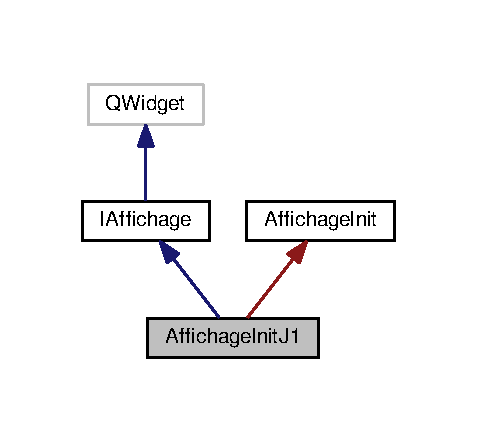
\includegraphics[width=229pt]{classAffichageInitJ1__inherit__graph}
\end{center}
\end{figure}


Collaboration diagram for Affichage\+Init\+J1\+:
\nopagebreak
\begin{figure}[H]
\begin{center}
\leavevmode
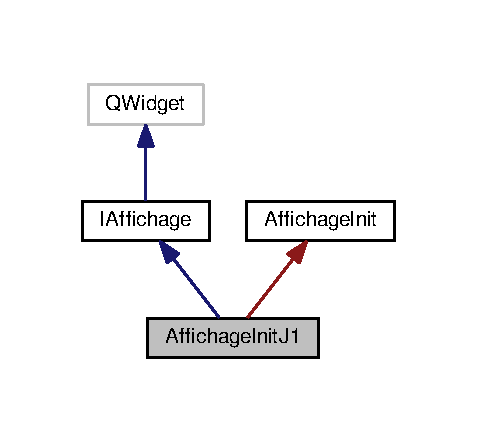
\includegraphics[width=229pt]{classAffichageInitJ1__coll__graph}
\end{center}
\end{figure}
\subsection*{Public Slots}
\begin{DoxyCompactItemize}
\item 
void \hyperlink{classAffichageInitJ1_a0ff516a3f3cc659cfb47e489076e99ac}{clic\+Bouton} ()
\begin{DoxyCompactList}\small\item\em Action pour le bouton \char`\"{}\+Pret\char`\"{}. \end{DoxyCompactList}\item 
void \hyperlink{classAffichageInitJ1_a785223ce5e31cc613821618c569210ca}{reset\+Carte\+Init} ()
\begin{DoxyCompactList}\small\item\em Action pour reset la carte. \end{DoxyCompactList}\end{DoxyCompactItemize}
\subsection*{Public Member Functions}
\begin{DoxyCompactItemize}
\item 
\hyperlink{classAffichageInitJ1_ac184edfaeebae278b71348584817cf3f}{Affichage\+Init\+J1} (\hyperlink{classCore}{Core} $\ast$c)
\begin{DoxyCompactList}\small\item\em Constructeur. \end{DoxyCompactList}\item 
void \hyperlink{classAffichageInitJ1_a469000a4072c712f88ee75ed6cc03d3b}{afficher} ()
\begin{DoxyCompactList}\small\item\em Affiche la fenêtre. \end{DoxyCompactList}\item 
void \hyperlink{classAffichageInitJ1_ac579f8933a11bc3e49923d414b20acab}{change\+To\+Menu} ()
\begin{DoxyCompactList}\small\item\em Change la fenêtre vers le menu. \end{DoxyCompactList}\item 
void \hyperlink{classAffichageInitJ1_a07ee576320b2bd22733ac142fd10b14c}{change\+To\+Initialisation\+J1} ()
\begin{DoxyCompactList}\small\item\em Change la fenêtre vers l'initialisation pour le J1. \end{DoxyCompactList}\item 
void \hyperlink{classAffichageInitJ1_ad1f6286f0aa162fec476d69049a2c1a8}{change\+To\+Initialisation\+J2} ()
\begin{DoxyCompactList}\small\item\em Change la fenêtre vers l'initialisation pour le J2. \end{DoxyCompactList}\item 
void \hyperlink{classAffichageInitJ1_a4fcbe1401407498fc32e5cedf797a9e4}{change\+To\+Jeu} ()
\begin{DoxyCompactList}\small\item\em Change la fenêtre vers le jeu. \end{DoxyCompactList}\end{DoxyCompactItemize}
\subsection*{Additional Inherited Members}


\subsection{Detailed Description}
classe representant l'affichage de la phase d'initialisation du J1 

La classe gère l'affichage et le changement de ce dernier pour le J1 

\subsection{Constructor \& Destructor Documentation}
\hypertarget{classAffichageInitJ1_ac184edfaeebae278b71348584817cf3f}{\index{Affichage\+Init\+J1@{Affichage\+Init\+J1}!Affichage\+Init\+J1@{Affichage\+Init\+J1}}
\index{Affichage\+Init\+J1@{Affichage\+Init\+J1}!Affichage\+Init\+J1@{Affichage\+Init\+J1}}
\subsubsection[{Affichage\+Init\+J1}]{\setlength{\rightskip}{0pt plus 5cm}Affichage\+Init\+J1\+::\+Affichage\+Init\+J1 (
\begin{DoxyParamCaption}
\item[{{\bf Core} $\ast$}]{c}
\end{DoxyParamCaption}
)}}\label{classAffichageInitJ1_ac184edfaeebae278b71348584817cf3f}


Constructeur. 

Constructeur de la classe \hyperlink{classAffichageInitJ1}{Affichage\+Init\+J1}


\begin{DoxyParams}{Parameters}
{\em c} & \+: le \hyperlink{classCore}{Core} de l'application \\
\hline
\end{DoxyParams}


\subsection{Member Function Documentation}
\hypertarget{classAffichageInitJ1_a469000a4072c712f88ee75ed6cc03d3b}{\index{Affichage\+Init\+J1@{Affichage\+Init\+J1}!afficher@{afficher}}
\index{afficher@{afficher}!Affichage\+Init\+J1@{Affichage\+Init\+J1}}
\subsubsection[{afficher}]{\setlength{\rightskip}{0pt plus 5cm}void Affichage\+Init\+J1\+::afficher (
\begin{DoxyParamCaption}
{}
\end{DoxyParamCaption}
)\hspace{0.3cm}{\ttfamily [virtual]}}}\label{classAffichageInitJ1_a469000a4072c712f88ee75ed6cc03d3b}


Affiche la fenêtre. 

Méthode pour afficher la fenêtre concernant l'initialisation pour le J1 

Implements \hyperlink{classIAffichage_a87e168995340186305675343d4b769fe}{I\+Affichage}.

\hypertarget{classAffichageInitJ1_a07ee576320b2bd22733ac142fd10b14c}{\index{Affichage\+Init\+J1@{Affichage\+Init\+J1}!change\+To\+Initialisation\+J1@{change\+To\+Initialisation\+J1}}
\index{change\+To\+Initialisation\+J1@{change\+To\+Initialisation\+J1}!Affichage\+Init\+J1@{Affichage\+Init\+J1}}
\subsubsection[{change\+To\+Initialisation\+J1}]{\setlength{\rightskip}{0pt plus 5cm}void Affichage\+Init\+J1\+::change\+To\+Initialisation\+J1 (
\begin{DoxyParamCaption}
{}
\end{DoxyParamCaption}
)\hspace{0.3cm}{\ttfamily [virtual]}}}\label{classAffichageInitJ1_a07ee576320b2bd22733ac142fd10b14c}


Change la fenêtre vers l'initialisation pour le J1. 

Méthode pour switcher la fenêtre courante avec celle de l'initialisation du J1 Pas implémenté pour cette classe 

Implements \hyperlink{classIAffichage_ac03c56ab489b760b1e42af15ac421039}{I\+Affichage}.

\hypertarget{classAffichageInitJ1_ad1f6286f0aa162fec476d69049a2c1a8}{\index{Affichage\+Init\+J1@{Affichage\+Init\+J1}!change\+To\+Initialisation\+J2@{change\+To\+Initialisation\+J2}}
\index{change\+To\+Initialisation\+J2@{change\+To\+Initialisation\+J2}!Affichage\+Init\+J1@{Affichage\+Init\+J1}}
\subsubsection[{change\+To\+Initialisation\+J2}]{\setlength{\rightskip}{0pt plus 5cm}void Affichage\+Init\+J1\+::change\+To\+Initialisation\+J2 (
\begin{DoxyParamCaption}
{}
\end{DoxyParamCaption}
)\hspace{0.3cm}{\ttfamily [virtual]}}}\label{classAffichageInitJ1_ad1f6286f0aa162fec476d69049a2c1a8}


Change la fenêtre vers l'initialisation pour le J2. 

Méthode pour switcher la fenêtre courante avec celle de l'initialisation du J2 

Implements \hyperlink{classIAffichage_a425bcafe36ba332f2cbc4badc99e19c2}{I\+Affichage}.

\hypertarget{classAffichageInitJ1_a4fcbe1401407498fc32e5cedf797a9e4}{\index{Affichage\+Init\+J1@{Affichage\+Init\+J1}!change\+To\+Jeu@{change\+To\+Jeu}}
\index{change\+To\+Jeu@{change\+To\+Jeu}!Affichage\+Init\+J1@{Affichage\+Init\+J1}}
\subsubsection[{change\+To\+Jeu}]{\setlength{\rightskip}{0pt plus 5cm}void Affichage\+Init\+J1\+::change\+To\+Jeu (
\begin{DoxyParamCaption}
{}
\end{DoxyParamCaption}
)\hspace{0.3cm}{\ttfamily [virtual]}}}\label{classAffichageInitJ1_a4fcbe1401407498fc32e5cedf797a9e4}


Change la fenêtre vers le jeu. 

Méthode pour switcher la fenêtre courante avec celle du jeu Pas implémenté pour cette classe 

Implements \hyperlink{classIAffichage_a52e20907ed94e272c592429d95fa5165}{I\+Affichage}.

\hypertarget{classAffichageInitJ1_ac579f8933a11bc3e49923d414b20acab}{\index{Affichage\+Init\+J1@{Affichage\+Init\+J1}!change\+To\+Menu@{change\+To\+Menu}}
\index{change\+To\+Menu@{change\+To\+Menu}!Affichage\+Init\+J1@{Affichage\+Init\+J1}}
\subsubsection[{change\+To\+Menu}]{\setlength{\rightskip}{0pt plus 5cm}void Affichage\+Init\+J1\+::change\+To\+Menu (
\begin{DoxyParamCaption}
{}
\end{DoxyParamCaption}
)\hspace{0.3cm}{\ttfamily [virtual]}}}\label{classAffichageInitJ1_ac579f8933a11bc3e49923d414b20acab}


Change la fenêtre vers le menu. 

Méthode pour switcher la fenêtre courante avec celle du menu Pas implémenté pour cette classe 

Implements \hyperlink{classIAffichage_a147a42f3068b7dc51d5a196252e53a39}{I\+Affichage}.

\hypertarget{classAffichageInitJ1_a0ff516a3f3cc659cfb47e489076e99ac}{\index{Affichage\+Init\+J1@{Affichage\+Init\+J1}!clic\+Bouton@{clic\+Bouton}}
\index{clic\+Bouton@{clic\+Bouton}!Affichage\+Init\+J1@{Affichage\+Init\+J1}}
\subsubsection[{clic\+Bouton}]{\setlength{\rightskip}{0pt plus 5cm}void Affichage\+Init\+J1\+::clic\+Bouton (
\begin{DoxyParamCaption}
{}
\end{DoxyParamCaption}
)\hspace{0.3cm}{\ttfamily [slot]}}}\label{classAffichageInitJ1_a0ff516a3f3cc659cfb47e489076e99ac}


Action pour le bouton \char`\"{}\+Pret\char`\"{}. 

Méthode pour passer à l'étape suivante (ici, soit init\+J2 pour le mode 1\+V1 soit jeu pour le mode 1\+V\+I\+A) \hypertarget{classAffichageInitJ1_a785223ce5e31cc613821618c569210ca}{\index{Affichage\+Init\+J1@{Affichage\+Init\+J1}!reset\+Carte\+Init@{reset\+Carte\+Init}}
\index{reset\+Carte\+Init@{reset\+Carte\+Init}!Affichage\+Init\+J1@{Affichage\+Init\+J1}}
\subsubsection[{reset\+Carte\+Init}]{\setlength{\rightskip}{0pt plus 5cm}void Affichage\+Init\+J1\+::reset\+Carte\+Init (
\begin{DoxyParamCaption}
{}
\end{DoxyParamCaption}
)\hspace{0.3cm}{\ttfamily [slot]}}}\label{classAffichageInitJ1_a785223ce5e31cc613821618c569210ca}


Action pour reset la carte. 

Méthode pour réinitialiser la carte en enlevant les bateaux présent pour les replacer 

The documentation for this class was generated from the following files\+:\begin{DoxyCompactItemize}
\item 
affichageinitj1.\+h\item 
affichageinitj1.\+cpp\end{DoxyCompactItemize}

\hypertarget{classAffichageInitJ2}{\section{Affichage\+Init\+J2 Class Reference}
\label{classAffichageInitJ2}\index{Affichage\+Init\+J2@{Affichage\+Init\+J2}}
}


classe representant l'affichage de la phase d'initialisation du J2  




{\ttfamily \#include $<$affichageinitj2.\+h$>$}



Inheritance diagram for Affichage\+Init\+J2\+:
\nopagebreak
\begin{figure}[H]
\begin{center}
\leavevmode
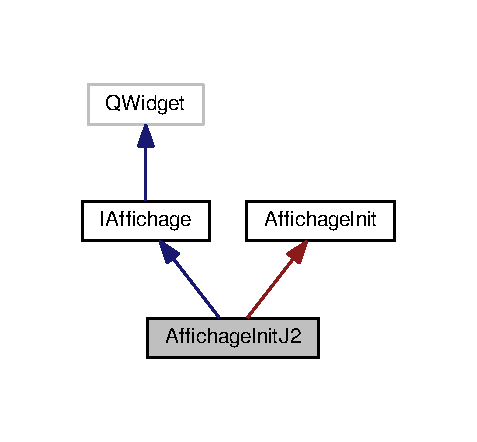
\includegraphics[width=229pt]{classAffichageInitJ2__inherit__graph}
\end{center}
\end{figure}


Collaboration diagram for Affichage\+Init\+J2\+:
\nopagebreak
\begin{figure}[H]
\begin{center}
\leavevmode
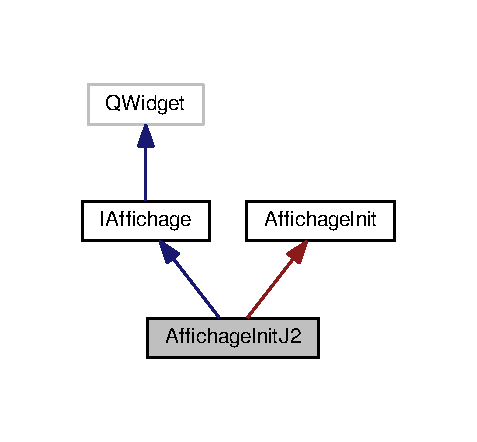
\includegraphics[width=229pt]{classAffichageInitJ2__coll__graph}
\end{center}
\end{figure}
\subsection*{Public Slots}
\begin{DoxyCompactItemize}
\item 
void \hyperlink{classAffichageInitJ2_ae8ff375ea33c514c71b5500d7d985e00}{clic\+Bouton} ()
\begin{DoxyCompactList}\small\item\em Action pour le bouton \char`\"{}\+Pret\char`\"{}. \end{DoxyCompactList}\item 
void \hyperlink{classAffichageInitJ2_abc45e1837c1612033c6c577a4825769a}{reset\+Carte\+Init} ()
\begin{DoxyCompactList}\small\item\em Action pour reset la carte. \end{DoxyCompactList}\end{DoxyCompactItemize}
\subsection*{Public Member Functions}
\begin{DoxyCompactItemize}
\item 
\hyperlink{classAffichageInitJ2_a8f9a34591f3e24cc990cccb66334bb35}{Affichage\+Init\+J2} (\hyperlink{classCore}{Core} $\ast$c)
\begin{DoxyCompactList}\small\item\em Constructeur. \end{DoxyCompactList}\item 
void \hyperlink{classAffichageInitJ2_a4b5dbe3833780c14aaaf946a7542e085}{afficher} ()
\begin{DoxyCompactList}\small\item\em Affiche la fenêtre. \end{DoxyCompactList}\item 
void \hyperlink{classAffichageInitJ2_a7266e6ce2188930080dc3ede1322d14d}{change\+To\+Menu} ()
\begin{DoxyCompactList}\small\item\em Change la fenêtre vers le menu. \end{DoxyCompactList}\item 
void \hyperlink{classAffichageInitJ2_a355056fd45cd18a199801eaf20181edc}{change\+To\+Initialisation\+J1} ()
\begin{DoxyCompactList}\small\item\em Change la fenêtre vers l'initialisation pour le J2. \end{DoxyCompactList}\item 
void \hyperlink{classAffichageInitJ2_a7f861d5e94c8ff21aae5b05601678292}{change\+To\+Initialisation\+J2} ()
\begin{DoxyCompactList}\small\item\em Change la fenêtre vers l'initialisation pour le J2. \end{DoxyCompactList}\item 
void \hyperlink{classAffichageInitJ2_ab2af503532ad81094f890d887bdb4f23}{change\+To\+Jeu} ()
\begin{DoxyCompactList}\small\item\em Change la fenêtre vers le jeu. \end{DoxyCompactList}\end{DoxyCompactItemize}
\subsection*{Additional Inherited Members}


\subsection{Detailed Description}
classe representant l'affichage de la phase d'initialisation du J2 

La classe gère l'affichage et le changement de ce dernier pour le J2 

\subsection{Constructor \& Destructor Documentation}
\hypertarget{classAffichageInitJ2_a8f9a34591f3e24cc990cccb66334bb35}{\index{Affichage\+Init\+J2@{Affichage\+Init\+J2}!Affichage\+Init\+J2@{Affichage\+Init\+J2}}
\index{Affichage\+Init\+J2@{Affichage\+Init\+J2}!Affichage\+Init\+J2@{Affichage\+Init\+J2}}
\subsubsection[{Affichage\+Init\+J2}]{\setlength{\rightskip}{0pt plus 5cm}Affichage\+Init\+J2\+::\+Affichage\+Init\+J2 (
\begin{DoxyParamCaption}
\item[{{\bf Core} $\ast$}]{c}
\end{DoxyParamCaption}
)}}\label{classAffichageInitJ2_a8f9a34591f3e24cc990cccb66334bb35}


Constructeur. 

Constructeur de la classe \hyperlink{classAffichageInitJ2}{Affichage\+Init\+J2}


\begin{DoxyParams}{Parameters}
{\em c} & \+: le \hyperlink{classCore}{Core} de l'application \\
\hline
\end{DoxyParams}


\subsection{Member Function Documentation}
\hypertarget{classAffichageInitJ2_a4b5dbe3833780c14aaaf946a7542e085}{\index{Affichage\+Init\+J2@{Affichage\+Init\+J2}!afficher@{afficher}}
\index{afficher@{afficher}!Affichage\+Init\+J2@{Affichage\+Init\+J2}}
\subsubsection[{afficher}]{\setlength{\rightskip}{0pt plus 5cm}void Affichage\+Init\+J2\+::afficher (
\begin{DoxyParamCaption}
{}
\end{DoxyParamCaption}
)\hspace{0.3cm}{\ttfamily [virtual]}}}\label{classAffichageInitJ2_a4b5dbe3833780c14aaaf946a7542e085}


Affiche la fenêtre. 

Méthode pour afficher la fenêtre concernant l'initialisation pour le J2 

Implements \hyperlink{classIAffichage_a87e168995340186305675343d4b769fe}{I\+Affichage}.

\hypertarget{classAffichageInitJ2_a355056fd45cd18a199801eaf20181edc}{\index{Affichage\+Init\+J2@{Affichage\+Init\+J2}!change\+To\+Initialisation\+J1@{change\+To\+Initialisation\+J1}}
\index{change\+To\+Initialisation\+J1@{change\+To\+Initialisation\+J1}!Affichage\+Init\+J2@{Affichage\+Init\+J2}}
\subsubsection[{change\+To\+Initialisation\+J1}]{\setlength{\rightskip}{0pt plus 5cm}void Affichage\+Init\+J2\+::change\+To\+Initialisation\+J1 (
\begin{DoxyParamCaption}
{}
\end{DoxyParamCaption}
)\hspace{0.3cm}{\ttfamily [virtual]}}}\label{classAffichageInitJ2_a355056fd45cd18a199801eaf20181edc}


Change la fenêtre vers l'initialisation pour le J2. 

Méthode pour switcher la fenêtre courante avec celle de l'initialisation du J2 Pas implémenté pour cette classe 

Implements \hyperlink{classIAffichage_ac03c56ab489b760b1e42af15ac421039}{I\+Affichage}.

\hypertarget{classAffichageInitJ2_a7f861d5e94c8ff21aae5b05601678292}{\index{Affichage\+Init\+J2@{Affichage\+Init\+J2}!change\+To\+Initialisation\+J2@{change\+To\+Initialisation\+J2}}
\index{change\+To\+Initialisation\+J2@{change\+To\+Initialisation\+J2}!Affichage\+Init\+J2@{Affichage\+Init\+J2}}
\subsubsection[{change\+To\+Initialisation\+J2}]{\setlength{\rightskip}{0pt plus 5cm}void Affichage\+Init\+J2\+::change\+To\+Initialisation\+J2 (
\begin{DoxyParamCaption}
{}
\end{DoxyParamCaption}
)\hspace{0.3cm}{\ttfamily [virtual]}}}\label{classAffichageInitJ2_a7f861d5e94c8ff21aae5b05601678292}


Change la fenêtre vers l'initialisation pour le J2. 

Méthode pour switcher la fenêtre courante avec celle de l'initialisation du J2 Pas implémenté pour cette classe 

Implements \hyperlink{classIAffichage_a425bcafe36ba332f2cbc4badc99e19c2}{I\+Affichage}.

\hypertarget{classAffichageInitJ2_ab2af503532ad81094f890d887bdb4f23}{\index{Affichage\+Init\+J2@{Affichage\+Init\+J2}!change\+To\+Jeu@{change\+To\+Jeu}}
\index{change\+To\+Jeu@{change\+To\+Jeu}!Affichage\+Init\+J2@{Affichage\+Init\+J2}}
\subsubsection[{change\+To\+Jeu}]{\setlength{\rightskip}{0pt plus 5cm}void Affichage\+Init\+J2\+::change\+To\+Jeu (
\begin{DoxyParamCaption}
{}
\end{DoxyParamCaption}
)\hspace{0.3cm}{\ttfamily [virtual]}}}\label{classAffichageInitJ2_ab2af503532ad81094f890d887bdb4f23}


Change la fenêtre vers le jeu. 

Méthode pour switcher la fenêtre courante avec celle du jeu 

Implements \hyperlink{classIAffichage_a52e20907ed94e272c592429d95fa5165}{I\+Affichage}.

\hypertarget{classAffichageInitJ2_a7266e6ce2188930080dc3ede1322d14d}{\index{Affichage\+Init\+J2@{Affichage\+Init\+J2}!change\+To\+Menu@{change\+To\+Menu}}
\index{change\+To\+Menu@{change\+To\+Menu}!Affichage\+Init\+J2@{Affichage\+Init\+J2}}
\subsubsection[{change\+To\+Menu}]{\setlength{\rightskip}{0pt plus 5cm}void Affichage\+Init\+J2\+::change\+To\+Menu (
\begin{DoxyParamCaption}
{}
\end{DoxyParamCaption}
)\hspace{0.3cm}{\ttfamily [virtual]}}}\label{classAffichageInitJ2_a7266e6ce2188930080dc3ede1322d14d}


Change la fenêtre vers le menu. 

Méthode pour switcher la fenêtre courante avec celle du menu Pas implémenté pour cette classe 

Implements \hyperlink{classIAffichage_a147a42f3068b7dc51d5a196252e53a39}{I\+Affichage}.

\hypertarget{classAffichageInitJ2_ae8ff375ea33c514c71b5500d7d985e00}{\index{Affichage\+Init\+J2@{Affichage\+Init\+J2}!clic\+Bouton@{clic\+Bouton}}
\index{clic\+Bouton@{clic\+Bouton}!Affichage\+Init\+J2@{Affichage\+Init\+J2}}
\subsubsection[{clic\+Bouton}]{\setlength{\rightskip}{0pt plus 5cm}void Affichage\+Init\+J2\+::clic\+Bouton (
\begin{DoxyParamCaption}
{}
\end{DoxyParamCaption}
)\hspace{0.3cm}{\ttfamily [slot]}}}\label{classAffichageInitJ2_ae8ff375ea33c514c71b5500d7d985e00}


Action pour le bouton \char`\"{}\+Pret\char`\"{}. 

Méthode pour passer à l'étape suivante (ici, jeu) \hypertarget{classAffichageInitJ2_abc45e1837c1612033c6c577a4825769a}{\index{Affichage\+Init\+J2@{Affichage\+Init\+J2}!reset\+Carte\+Init@{reset\+Carte\+Init}}
\index{reset\+Carte\+Init@{reset\+Carte\+Init}!Affichage\+Init\+J2@{Affichage\+Init\+J2}}
\subsubsection[{reset\+Carte\+Init}]{\setlength{\rightskip}{0pt plus 5cm}void Affichage\+Init\+J2\+::reset\+Carte\+Init (
\begin{DoxyParamCaption}
{}
\end{DoxyParamCaption}
)\hspace{0.3cm}{\ttfamily [slot]}}}\label{classAffichageInitJ2_abc45e1837c1612033c6c577a4825769a}


Action pour reset la carte. 

Méthode pour réinitialiser la carte en enlevant les bateaux présent pour les replacer 

The documentation for this class was generated from the following files\+:\begin{DoxyCompactItemize}
\item 
affichageinitj2.\+h\item 
affichageinitj2.\+cpp\end{DoxyCompactItemize}

\hypertarget{classAffichageJeu}{\section{Affichage\+Jeu Class Reference}
\label{classAffichageJeu}\index{Affichage\+Jeu@{Affichage\+Jeu}}
}


classe representant l'affichage du jeu  




{\ttfamily \#include $<$affichagejeu.\+h$>$}



Inheritance diagram for Affichage\+Jeu\+:
\nopagebreak
\begin{figure}[H]
\begin{center}
\leavevmode
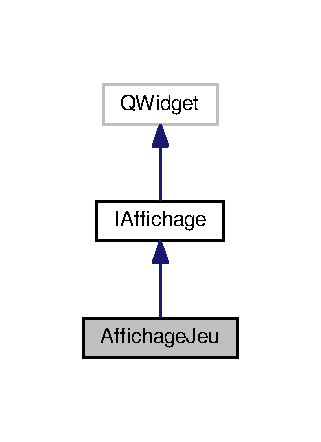
\includegraphics[width=154pt]{classAffichageJeu__inherit__graph}
\end{center}
\end{figure}


Collaboration diagram for Affichage\+Jeu\+:
\nopagebreak
\begin{figure}[H]
\begin{center}
\leavevmode
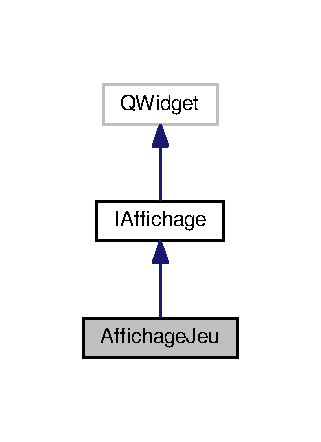
\includegraphics[width=154pt]{classAffichageJeu__coll__graph}
\end{center}
\end{figure}
\subsection*{Public Member Functions}
\begin{DoxyCompactItemize}
\item 
\hyperlink{classAffichageJeu_a2aadf21ada8d8a8d2af275842e9fbda2}{Affichage\+Jeu} (\hyperlink{classCore}{Core} $\ast$c)
\begin{DoxyCompactList}\small\item\em Constructeur. \end{DoxyCompactList}\item 
void \hyperlink{classAffichageJeu_a29d9ad7ef0161faa698bd0850efbb1fc}{afficher} ()
\begin{DoxyCompactList}\small\item\em Affiche la fenêtre. \end{DoxyCompactList}\item 
void \hyperlink{classAffichageJeu_ad17e5eea2e70c327f085b6e0ed9330e4}{update\+Elements} ()
\begin{DoxyCompactList}\small\item\em Ajout de tous les éléments pour l'affichage. \end{DoxyCompactList}\item 
void \hyperlink{classAffichageJeu_aa0fe30f907b9c0c2007466d287c701fd}{change\+To\+Menu} ()
\begin{DoxyCompactList}\small\item\em Change la fenêtre vers le menu. \end{DoxyCompactList}\item 
void \hyperlink{classAffichageJeu_a4e8693c20861bc9e79e0c0037ba4ffa8}{change\+To\+Initialisation\+J1} ()
\begin{DoxyCompactList}\small\item\em Change la fenêtre vers l'initialisation pour le J1. \end{DoxyCompactList}\item 
void \hyperlink{classAffichageJeu_a62db45f512fb855b096bcfd19e379429}{change\+To\+Initialisation\+J2} ()
\begin{DoxyCompactList}\small\item\em Change la fenêtre vers l'initialisation pour le J2. \end{DoxyCompactList}\item 
void \hyperlink{classAffichageJeu_aec00eea36f08e0bd187832d17ec32680}{change\+To\+Jeu} ()
\begin{DoxyCompactList}\small\item\em Change la fenêtre vers le jeu. \end{DoxyCompactList}\item 
void \hyperlink{classAffichageJeu_aa04e21a18ec82b601605a6ca974ea6d7}{add\+Content} (Q\+Widget $\ast$c, int x, int y)
\begin{DoxyCompactList}\small\item\em Ajouter des widgets à l'affichage. \end{DoxyCompactList}\item 
void \hyperlink{classAffichageJeu_aacb8b0c827d1b623e082546a7a461e11}{set\+Image\+Chgmt\+Tour} ()
\begin{DoxyCompactList}\small\item\em Changer le sens de l'image du tour du joueur. \end{DoxyCompactList}\item 
std\+::shared\+\_\+ptr$<$ \hyperlink{classCarte}{Carte} $>$ \hyperlink{classAffichageJeu_a28cf87eb40e06577ce095413ab1933cf}{get\+Carte\+Jeu\+T1} ()
\begin{DoxyCompactList}\small\item\em Récupère la carte d'initialisation du J1. \end{DoxyCompactList}\item 
std\+::shared\+\_\+ptr$<$ \hyperlink{classCarte}{Carte} $>$ \hyperlink{classAffichageJeu_a8604b85fd85bca4fd7ec1bce8c012d93}{get\+Carte\+Jeu\+T2} ()
\begin{DoxyCompactList}\small\item\em Récupère la carte d'initialisation du J2. \end{DoxyCompactList}\end{DoxyCompactItemize}
\subsection*{Additional Inherited Members}


\subsection{Detailed Description}
classe representant l'affichage du jeu 

La classe gère l'affichage du jeu avec les deux cartes et les autres éléments 

\subsection{Constructor \& Destructor Documentation}
\hypertarget{classAffichageJeu_a2aadf21ada8d8a8d2af275842e9fbda2}{\index{Affichage\+Jeu@{Affichage\+Jeu}!Affichage\+Jeu@{Affichage\+Jeu}}
\index{Affichage\+Jeu@{Affichage\+Jeu}!Affichage\+Jeu@{Affichage\+Jeu}}
\subsubsection[{Affichage\+Jeu}]{\setlength{\rightskip}{0pt plus 5cm}Affichage\+Jeu\+::\+Affichage\+Jeu (
\begin{DoxyParamCaption}
\item[{{\bf Core} $\ast$}]{c}
\end{DoxyParamCaption}
)}}\label{classAffichageJeu_a2aadf21ada8d8a8d2af275842e9fbda2}


Constructeur. 

Constructeur de la classe \hyperlink{classAffichageJeu}{Affichage\+Jeu}


\begin{DoxyParams}{Parameters}
{\em c} & \+: le \hyperlink{classCore}{Core} de l'application \\
\hline
\end{DoxyParams}


\subsection{Member Function Documentation}
\hypertarget{classAffichageJeu_aa04e21a18ec82b601605a6ca974ea6d7}{\index{Affichage\+Jeu@{Affichage\+Jeu}!add\+Content@{add\+Content}}
\index{add\+Content@{add\+Content}!Affichage\+Jeu@{Affichage\+Jeu}}
\subsubsection[{add\+Content}]{\setlength{\rightskip}{0pt plus 5cm}void Affichage\+Jeu\+::add\+Content (
\begin{DoxyParamCaption}
\item[{Q\+Widget $\ast$}]{c, }
\item[{int}]{x, }
\item[{int}]{y}
\end{DoxyParamCaption}
)}}\label{classAffichageJeu_aa04e21a18ec82b601605a6ca974ea6d7}


Ajouter des widgets à l'affichage. 

Méthode permettant d'ajouter les cartes à l'affichages on peut ajouter n'importe quel élément


\begin{DoxyParams}{Parameters}
{\em c} & \+: l'élément à ajouter \\
\hline
{\em x} & \+: le n° ligne dans le layout \\
\hline
{\em y} & \+: le n° colonne dans le layout \\
\hline
\end{DoxyParams}
\hypertarget{classAffichageJeu_a29d9ad7ef0161faa698bd0850efbb1fc}{\index{Affichage\+Jeu@{Affichage\+Jeu}!afficher@{afficher}}
\index{afficher@{afficher}!Affichage\+Jeu@{Affichage\+Jeu}}
\subsubsection[{afficher}]{\setlength{\rightskip}{0pt plus 5cm}void Affichage\+Jeu\+::afficher (
\begin{DoxyParamCaption}
{}
\end{DoxyParamCaption}
)\hspace{0.3cm}{\ttfamily [virtual]}}}\label{classAffichageJeu_a29d9ad7ef0161faa698bd0850efbb1fc}


Affiche la fenêtre. 

Méthode pour afficher la fenêtre concernant le jeu 

Implements \hyperlink{classIAffichage_a87e168995340186305675343d4b769fe}{I\+Affichage}.

\hypertarget{classAffichageJeu_a4e8693c20861bc9e79e0c0037ba4ffa8}{\index{Affichage\+Jeu@{Affichage\+Jeu}!change\+To\+Initialisation\+J1@{change\+To\+Initialisation\+J1}}
\index{change\+To\+Initialisation\+J1@{change\+To\+Initialisation\+J1}!Affichage\+Jeu@{Affichage\+Jeu}}
\subsubsection[{change\+To\+Initialisation\+J1}]{\setlength{\rightskip}{0pt plus 5cm}void Affichage\+Jeu\+::change\+To\+Initialisation\+J1 (
\begin{DoxyParamCaption}
{}
\end{DoxyParamCaption}
)\hspace{0.3cm}{\ttfamily [virtual]}}}\label{classAffichageJeu_a4e8693c20861bc9e79e0c0037ba4ffa8}


Change la fenêtre vers l'initialisation pour le J1. 

Méthode pour switcher la fenêtre courante avec celle de l'initialisation du J1 Pas implémenté pour cette classe 

Implements \hyperlink{classIAffichage_ac03c56ab489b760b1e42af15ac421039}{I\+Affichage}.

\hypertarget{classAffichageJeu_a62db45f512fb855b096bcfd19e379429}{\index{Affichage\+Jeu@{Affichage\+Jeu}!change\+To\+Initialisation\+J2@{change\+To\+Initialisation\+J2}}
\index{change\+To\+Initialisation\+J2@{change\+To\+Initialisation\+J2}!Affichage\+Jeu@{Affichage\+Jeu}}
\subsubsection[{change\+To\+Initialisation\+J2}]{\setlength{\rightskip}{0pt plus 5cm}void Affichage\+Jeu\+::change\+To\+Initialisation\+J2 (
\begin{DoxyParamCaption}
{}
\end{DoxyParamCaption}
)\hspace{0.3cm}{\ttfamily [virtual]}}}\label{classAffichageJeu_a62db45f512fb855b096bcfd19e379429}


Change la fenêtre vers l'initialisation pour le J2. 

Méthode pour switcher la fenêtre courante avec celle de l'initialisation du J2 Pas implémenté pour cette classe 

Implements \hyperlink{classIAffichage_a425bcafe36ba332f2cbc4badc99e19c2}{I\+Affichage}.

\hypertarget{classAffichageJeu_aec00eea36f08e0bd187832d17ec32680}{\index{Affichage\+Jeu@{Affichage\+Jeu}!change\+To\+Jeu@{change\+To\+Jeu}}
\index{change\+To\+Jeu@{change\+To\+Jeu}!Affichage\+Jeu@{Affichage\+Jeu}}
\subsubsection[{change\+To\+Jeu}]{\setlength{\rightskip}{0pt plus 5cm}void Affichage\+Jeu\+::change\+To\+Jeu (
\begin{DoxyParamCaption}
{}
\end{DoxyParamCaption}
)\hspace{0.3cm}{\ttfamily [virtual]}}}\label{classAffichageJeu_aec00eea36f08e0bd187832d17ec32680}


Change la fenêtre vers le jeu. 

Méthode pour switcher la fenêtre courante avec celle du jeu Pas implémenté pour cette classe 

Implements \hyperlink{classIAffichage_a52e20907ed94e272c592429d95fa5165}{I\+Affichage}.

\hypertarget{classAffichageJeu_aa0fe30f907b9c0c2007466d287c701fd}{\index{Affichage\+Jeu@{Affichage\+Jeu}!change\+To\+Menu@{change\+To\+Menu}}
\index{change\+To\+Menu@{change\+To\+Menu}!Affichage\+Jeu@{Affichage\+Jeu}}
\subsubsection[{change\+To\+Menu}]{\setlength{\rightskip}{0pt plus 5cm}void Affichage\+Jeu\+::change\+To\+Menu (
\begin{DoxyParamCaption}
{}
\end{DoxyParamCaption}
)\hspace{0.3cm}{\ttfamily [virtual]}}}\label{classAffichageJeu_aa0fe30f907b9c0c2007466d287c701fd}


Change la fenêtre vers le menu. 

Méthode pour switcher la fenêtre courante avec celle du menu Pas implémenté pour cette classe 

Implements \hyperlink{classIAffichage_a147a42f3068b7dc51d5a196252e53a39}{I\+Affichage}.

\hypertarget{classAffichageJeu_a28cf87eb40e06577ce095413ab1933cf}{\index{Affichage\+Jeu@{Affichage\+Jeu}!get\+Carte\+Jeu\+T1@{get\+Carte\+Jeu\+T1}}
\index{get\+Carte\+Jeu\+T1@{get\+Carte\+Jeu\+T1}!Affichage\+Jeu@{Affichage\+Jeu}}
\subsubsection[{get\+Carte\+Jeu\+T1}]{\setlength{\rightskip}{0pt plus 5cm}std\+::shared\+\_\+ptr$<$ {\bf Carte} $>$ Affichage\+Jeu\+::get\+Carte\+Jeu\+T1 (
\begin{DoxyParamCaption}
{}
\end{DoxyParamCaption}
)}}\label{classAffichageJeu_a28cf87eb40e06577ce095413ab1933cf}


Récupère la carte d'initialisation du J1. 

Methode qui permet de retourner la carte d'initialisation du J1 avec tous ses bateaux

\begin{DoxyReturn}{Returns}
la carte d'initialisation du J1 
\end{DoxyReturn}
\hypertarget{classAffichageJeu_a8604b85fd85bca4fd7ec1bce8c012d93}{\index{Affichage\+Jeu@{Affichage\+Jeu}!get\+Carte\+Jeu\+T2@{get\+Carte\+Jeu\+T2}}
\index{get\+Carte\+Jeu\+T2@{get\+Carte\+Jeu\+T2}!Affichage\+Jeu@{Affichage\+Jeu}}
\subsubsection[{get\+Carte\+Jeu\+T2}]{\setlength{\rightskip}{0pt plus 5cm}std\+::shared\+\_\+ptr$<$ {\bf Carte} $>$ Affichage\+Jeu\+::get\+Carte\+Jeu\+T2 (
\begin{DoxyParamCaption}
{}
\end{DoxyParamCaption}
)}}\label{classAffichageJeu_a8604b85fd85bca4fd7ec1bce8c012d93}


Récupère la carte d'initialisation du J2. 

Methode qui permet de retourner la carte d'initialisation du J2 avec tous ses bateaux

\begin{DoxyReturn}{Returns}
la carte d'initialisation du J2 
\end{DoxyReturn}
\hypertarget{classAffichageJeu_aacb8b0c827d1b623e082546a7a461e11}{\index{Affichage\+Jeu@{Affichage\+Jeu}!set\+Image\+Chgmt\+Tour@{set\+Image\+Chgmt\+Tour}}
\index{set\+Image\+Chgmt\+Tour@{set\+Image\+Chgmt\+Tour}!Affichage\+Jeu@{Affichage\+Jeu}}
\subsubsection[{set\+Image\+Chgmt\+Tour}]{\setlength{\rightskip}{0pt plus 5cm}void Affichage\+Jeu\+::set\+Image\+Chgmt\+Tour (
\begin{DoxyParamCaption}
{}
\end{DoxyParamCaption}
)}}\label{classAffichageJeu_aacb8b0c827d1b623e082546a7a461e11}


Changer le sens de l'image du tour du joueur. 

Méthode permettant de tourner de 180° le triangle indiquant à quel joueur est le tour \hypertarget{classAffichageJeu_ad17e5eea2e70c327f085b6e0ed9330e4}{\index{Affichage\+Jeu@{Affichage\+Jeu}!update\+Elements@{update\+Elements}}
\index{update\+Elements@{update\+Elements}!Affichage\+Jeu@{Affichage\+Jeu}}
\subsubsection[{update\+Elements}]{\setlength{\rightskip}{0pt plus 5cm}void Affichage\+Jeu\+::update\+Elements (
\begin{DoxyParamCaption}
{}
\end{DoxyParamCaption}
)}}\label{classAffichageJeu_ad17e5eea2e70c327f085b6e0ed9330e4}


Ajout de tous les éléments pour l'affichage. 

Methode qui permet d'ajouter l'ensemble des éléments pour l'affichage du jeu (la carte et les pseudos) 

The documentation for this class was generated from the following files\+:\begin{DoxyCompactItemize}
\item 
affichagejeu.\+h\item 
affichagejeu.\+cpp\end{DoxyCompactItemize}

\hypertarget{classAffichageMenu}{\section{Affichage\+Menu Class Reference}
\label{classAffichageMenu}\index{Affichage\+Menu@{Affichage\+Menu}}
}


classe representant l'affichage du menu  




{\ttfamily \#include $<$affichagemenu.\+h$>$}



Inheritance diagram for Affichage\+Menu\+:
\nopagebreak
\begin{figure}[H]
\begin{center}
\leavevmode
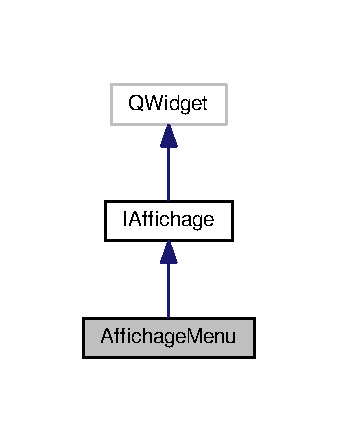
\includegraphics[width=162pt]{classAffichageMenu__inherit__graph}
\end{center}
\end{figure}


Collaboration diagram for Affichage\+Menu\+:
\nopagebreak
\begin{figure}[H]
\begin{center}
\leavevmode
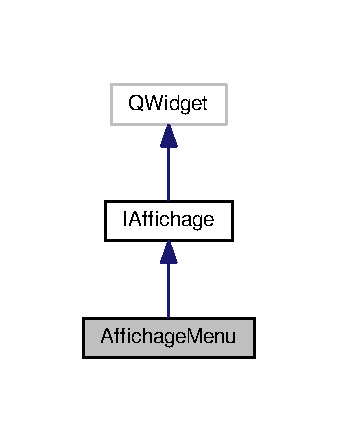
\includegraphics[width=162pt]{classAffichageMenu__coll__graph}
\end{center}
\end{figure}
\subsection*{Public Slots}
\begin{DoxyCompactItemize}
\item 
void \hyperlink{classAffichageMenu_ae62a39124cc5bb46805c464f23cd0ea0}{clic\+Mode1vs1} ()
\begin{DoxyCompactList}\small\item\em Action pour le mode 1\+V1. \end{DoxyCompactList}\item 
void \hyperlink{classAffichageMenu_a737cc4c685ddd031cad5286d513e9002}{clic\+Mode1vs\+I\+A} ()
\begin{DoxyCompactList}\small\item\em Action pour le mode 1\+V1. \end{DoxyCompactList}\end{DoxyCompactItemize}
\subsection*{Public Member Functions}
\begin{DoxyCompactItemize}
\item 
\hyperlink{classAffichageMenu_a68e70ec71422f3cb651299f08c85987e}{Affichage\+Menu} (\hyperlink{classCore}{Core} $\ast$c)
\begin{DoxyCompactList}\small\item\em Constructeur. \end{DoxyCompactList}\item 
void \hyperlink{classAffichageMenu_abec0adf6db92df26a937ff702a5a87fc}{afficher} ()
\begin{DoxyCompactList}\small\item\em Affiche la fenêtre. \end{DoxyCompactList}\item 
void \hyperlink{classAffichageMenu_a5f825906a1c5afccfbb03b007906bd28}{change\+To\+Menu} ()
\begin{DoxyCompactList}\small\item\em Change la fenêtre vers le menu. \end{DoxyCompactList}\item 
void \hyperlink{classAffichageMenu_ab7df249dc5db82d25613b80c28ba1ed4}{change\+To\+Initialisation\+J1} ()
\begin{DoxyCompactList}\small\item\em Change la fenêtre vers l'initialisation pour le J1. \end{DoxyCompactList}\item 
void \hyperlink{classAffichageMenu_a1980bc54a6156938cc3b737972facd32}{change\+To\+Initialisation\+J2} ()
\begin{DoxyCompactList}\small\item\em Change la fenêtre vers l'initialisation pour le J2. \end{DoxyCompactList}\item 
void \hyperlink{classAffichageMenu_a878a89a1ce7e138695e3e5fde5e020af}{change\+To\+Jeu} ()
\begin{DoxyCompactList}\small\item\em Change la fenêtre vers le jeu. \end{DoxyCompactList}\end{DoxyCompactItemize}
\subsection*{Protected Attributes}
\begin{DoxyCompactItemize}
\item 
Q\+V\+Box\+Layout $\ast$ \hyperlink{classAffichageMenu_a190c22c6af2b9d0f5f45b727a1f60838}{b\+Layout\+\_\+}
\item 
Q\+Grid\+Layout $\ast$ \hyperlink{classAffichageMenu_a33ee17880f8d6d985c19eebf0e5f121b}{g\+Layout\+\_\+}
\end{DoxyCompactItemize}


\subsection{Detailed Description}
classe representant l'affichage du menu 

La classe gère l'affichage des boutons de choix de jeu au sein du menu 

\subsection{Constructor \& Destructor Documentation}
\hypertarget{classAffichageMenu_a68e70ec71422f3cb651299f08c85987e}{\index{Affichage\+Menu@{Affichage\+Menu}!Affichage\+Menu@{Affichage\+Menu}}
\index{Affichage\+Menu@{Affichage\+Menu}!Affichage\+Menu@{Affichage\+Menu}}
\subsubsection[{Affichage\+Menu}]{\setlength{\rightskip}{0pt plus 5cm}Affichage\+Menu\+::\+Affichage\+Menu (
\begin{DoxyParamCaption}
\item[{{\bf Core} $\ast$}]{c}
\end{DoxyParamCaption}
)}}\label{classAffichageMenu_a68e70ec71422f3cb651299f08c85987e}


Constructeur. 

Constructeur de la classe \hyperlink{classAffichageMenu}{Affichage\+Menu}


\begin{DoxyParams}{Parameters}
{\em c} & \+: le \hyperlink{classCore}{Core} de l'application \\
\hline
\end{DoxyParams}


\subsection{Member Function Documentation}
\hypertarget{classAffichageMenu_abec0adf6db92df26a937ff702a5a87fc}{\index{Affichage\+Menu@{Affichage\+Menu}!afficher@{afficher}}
\index{afficher@{afficher}!Affichage\+Menu@{Affichage\+Menu}}
\subsubsection[{afficher}]{\setlength{\rightskip}{0pt plus 5cm}void Affichage\+Menu\+::afficher (
\begin{DoxyParamCaption}
{}
\end{DoxyParamCaption}
)\hspace{0.3cm}{\ttfamily [virtual]}}}\label{classAffichageMenu_abec0adf6db92df26a937ff702a5a87fc}


Affiche la fenêtre. 

Méthode pour afficher la fenêtre concernant le jeu 

Implements \hyperlink{classIAffichage_a87e168995340186305675343d4b769fe}{I\+Affichage}.

\hypertarget{classAffichageMenu_ab7df249dc5db82d25613b80c28ba1ed4}{\index{Affichage\+Menu@{Affichage\+Menu}!change\+To\+Initialisation\+J1@{change\+To\+Initialisation\+J1}}
\index{change\+To\+Initialisation\+J1@{change\+To\+Initialisation\+J1}!Affichage\+Menu@{Affichage\+Menu}}
\subsubsection[{change\+To\+Initialisation\+J1}]{\setlength{\rightskip}{0pt plus 5cm}void Affichage\+Menu\+::change\+To\+Initialisation\+J1 (
\begin{DoxyParamCaption}
{}
\end{DoxyParamCaption}
)\hspace{0.3cm}{\ttfamily [virtual]}}}\label{classAffichageMenu_ab7df249dc5db82d25613b80c28ba1ed4}


Change la fenêtre vers l'initialisation pour le J1. 

Méthode pour switcher la fenêtre courante avec celle de l'initialisation du J1 

Implements \hyperlink{classIAffichage_ac03c56ab489b760b1e42af15ac421039}{I\+Affichage}.

\hypertarget{classAffichageMenu_a1980bc54a6156938cc3b737972facd32}{\index{Affichage\+Menu@{Affichage\+Menu}!change\+To\+Initialisation\+J2@{change\+To\+Initialisation\+J2}}
\index{change\+To\+Initialisation\+J2@{change\+To\+Initialisation\+J2}!Affichage\+Menu@{Affichage\+Menu}}
\subsubsection[{change\+To\+Initialisation\+J2}]{\setlength{\rightskip}{0pt plus 5cm}void Affichage\+Menu\+::change\+To\+Initialisation\+J2 (
\begin{DoxyParamCaption}
{}
\end{DoxyParamCaption}
)\hspace{0.3cm}{\ttfamily [virtual]}}}\label{classAffichageMenu_a1980bc54a6156938cc3b737972facd32}


Change la fenêtre vers l'initialisation pour le J2. 

Méthode pour switcher la fenêtre courante avec celle de l'initialisation du J2 Pas implémenté pour cette classe 

Implements \hyperlink{classIAffichage_a425bcafe36ba332f2cbc4badc99e19c2}{I\+Affichage}.

\hypertarget{classAffichageMenu_a878a89a1ce7e138695e3e5fde5e020af}{\index{Affichage\+Menu@{Affichage\+Menu}!change\+To\+Jeu@{change\+To\+Jeu}}
\index{change\+To\+Jeu@{change\+To\+Jeu}!Affichage\+Menu@{Affichage\+Menu}}
\subsubsection[{change\+To\+Jeu}]{\setlength{\rightskip}{0pt plus 5cm}void Affichage\+Menu\+::change\+To\+Jeu (
\begin{DoxyParamCaption}
{}
\end{DoxyParamCaption}
)\hspace{0.3cm}{\ttfamily [virtual]}}}\label{classAffichageMenu_a878a89a1ce7e138695e3e5fde5e020af}


Change la fenêtre vers le jeu. 

Méthode pour switcher la fenêtre courante avec celle du jeu Pas implémenté pour cette classe 

Implements \hyperlink{classIAffichage_a52e20907ed94e272c592429d95fa5165}{I\+Affichage}.

\hypertarget{classAffichageMenu_a5f825906a1c5afccfbb03b007906bd28}{\index{Affichage\+Menu@{Affichage\+Menu}!change\+To\+Menu@{change\+To\+Menu}}
\index{change\+To\+Menu@{change\+To\+Menu}!Affichage\+Menu@{Affichage\+Menu}}
\subsubsection[{change\+To\+Menu}]{\setlength{\rightskip}{0pt plus 5cm}void Affichage\+Menu\+::change\+To\+Menu (
\begin{DoxyParamCaption}
{}
\end{DoxyParamCaption}
)\hspace{0.3cm}{\ttfamily [virtual]}}}\label{classAffichageMenu_a5f825906a1c5afccfbb03b007906bd28}


Change la fenêtre vers le menu. 

Méthode pour switcher la fenêtre courante avec celle du menu Pas implémenté pour cette classe 

Implements \hyperlink{classIAffichage_a147a42f3068b7dc51d5a196252e53a39}{I\+Affichage}.

\hypertarget{classAffichageMenu_ae62a39124cc5bb46805c464f23cd0ea0}{\index{Affichage\+Menu@{Affichage\+Menu}!clic\+Mode1vs1@{clic\+Mode1vs1}}
\index{clic\+Mode1vs1@{clic\+Mode1vs1}!Affichage\+Menu@{Affichage\+Menu}}
\subsubsection[{clic\+Mode1vs1}]{\setlength{\rightskip}{0pt plus 5cm}void Affichage\+Menu\+::clic\+Mode1vs1 (
\begin{DoxyParamCaption}
{}
\end{DoxyParamCaption}
)\hspace{0.3cm}{\ttfamily [slot]}}}\label{classAffichageMenu_ae62a39124cc5bb46805c464f23cd0ea0}


Action pour le mode 1\+V1. 

Méthode pour lancer le jeu avec le mode 1\+V1 \hypertarget{classAffichageMenu_a737cc4c685ddd031cad5286d513e9002}{\index{Affichage\+Menu@{Affichage\+Menu}!clic\+Mode1vs\+I\+A@{clic\+Mode1vs\+I\+A}}
\index{clic\+Mode1vs\+I\+A@{clic\+Mode1vs\+I\+A}!Affichage\+Menu@{Affichage\+Menu}}
\subsubsection[{clic\+Mode1vs\+I\+A}]{\setlength{\rightskip}{0pt plus 5cm}void Affichage\+Menu\+::clic\+Mode1vs\+I\+A (
\begin{DoxyParamCaption}
{}
\end{DoxyParamCaption}
)\hspace{0.3cm}{\ttfamily [slot]}}}\label{classAffichageMenu_a737cc4c685ddd031cad5286d513e9002}


Action pour le mode 1\+V1. 

Méthode pour lancer le jeu avec le mode 1\+V\+I\+A 

\subsection{Member Data Documentation}
\hypertarget{classAffichageMenu_a190c22c6af2b9d0f5f45b727a1f60838}{\index{Affichage\+Menu@{Affichage\+Menu}!b\+Layout\+\_\+@{b\+Layout\+\_\+}}
\index{b\+Layout\+\_\+@{b\+Layout\+\_\+}!Affichage\+Menu@{Affichage\+Menu}}
\subsubsection[{b\+Layout\+\_\+}]{\setlength{\rightskip}{0pt plus 5cm}Q\+V\+Box\+Layout$\ast$ Affichage\+Menu\+::b\+Layout\+\_\+\hspace{0.3cm}{\ttfamily [protected]}}}\label{classAffichageMenu_a190c22c6af2b9d0f5f45b727a1f60838}
layout contenant les boutons \hypertarget{classAffichageMenu_a33ee17880f8d6d985c19eebf0e5f121b}{\index{Affichage\+Menu@{Affichage\+Menu}!g\+Layout\+\_\+@{g\+Layout\+\_\+}}
\index{g\+Layout\+\_\+@{g\+Layout\+\_\+}!Affichage\+Menu@{Affichage\+Menu}}
\subsubsection[{g\+Layout\+\_\+}]{\setlength{\rightskip}{0pt plus 5cm}Q\+Grid\+Layout$\ast$ Affichage\+Menu\+::g\+Layout\+\_\+\hspace{0.3cm}{\ttfamily [protected]}}}\label{classAffichageMenu_a33ee17880f8d6d985c19eebf0e5f121b}
Layout principal 

The documentation for this class was generated from the following files\+:\begin{DoxyCompactItemize}
\item 
affichagemenu.\+h\item 
affichagemenu.\+cpp\end{DoxyCompactItemize}

\hypertarget{classBateau}{\section{Bateau Class Reference}
\label{classBateau}\index{Bateau@{Bateau}}
}


classe representant un \hyperlink{classBateau}{Bateau}  




{\ttfamily \#include $<$bateau.\+h$>$}



Inheritance diagram for Bateau\+:
\nopagebreak
\begin{figure}[H]
\begin{center}
\leavevmode
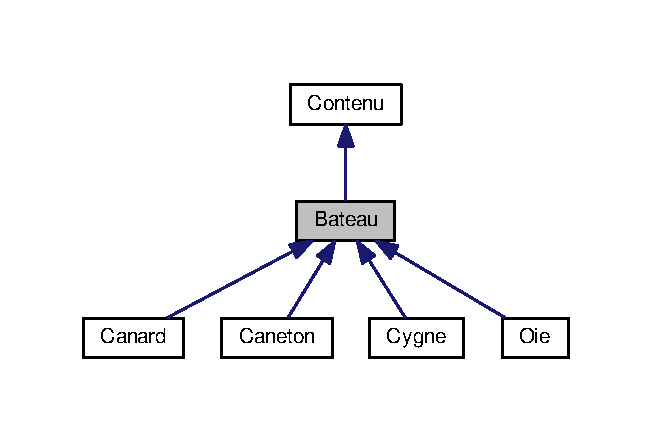
\includegraphics[width=313pt]{classBateau__inherit__graph}
\end{center}
\end{figure}


Collaboration diagram for Bateau\+:
\nopagebreak
\begin{figure}[H]
\begin{center}
\leavevmode
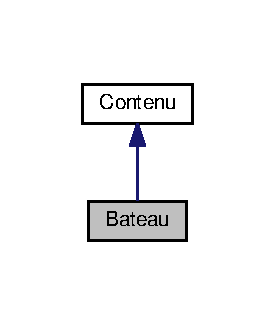
\includegraphics[width=132pt]{classBateau__coll__graph}
\end{center}
\end{figure}
\subsection*{Public Member Functions}
\begin{DoxyCompactItemize}
\item 
\hyperlink{classBateau_af9484dd811f8f678d92bfd70e2f1c5e2}{Bateau} (int taille)
\begin{DoxyCompactList}\small\item\em Constructeur. \end{DoxyCompactList}\item 
bool \hyperlink{classBateau_a3e54040953962f545b5fabadbcc330e8}{action} (\hyperlink{classCase}{Case} $\ast$c)
\begin{DoxyCompactList}\small\item\em Action émise lorsqu'on a cliqué sur un \hyperlink{classBateau}{Bateau}. \end{DoxyCompactList}\item 
void \hyperlink{classBateau_a12cc2226f5533d98b5b1f71fc042f1a6}{set\+X} (int x)
\begin{DoxyCompactList}\small\item\em Modifie la coordonnée X du \hyperlink{classBateau}{Bateau}. \end{DoxyCompactList}\item 
void \hyperlink{classBateau_ad84a941f5968a3690b80b12ca56547c4}{set\+Y} (int y)
\begin{DoxyCompactList}\small\item\em Modifie la coordonnée Y du \hyperlink{classBateau}{Bateau}. \end{DoxyCompactList}\item 
void \hyperlink{classBateau_a1dae1dbd3d3e0334a4dc5b43ef579c25}{set\+Horizontal} (bool a)
\begin{DoxyCompactList}\small\item\em Modifie l'orientation du \hyperlink{classBateau}{Bateau}. \end{DoxyCompactList}\item 
int \hyperlink{classBateau_ab7bd97ef05abea97c5322a16760b7d51}{get\+X} ()
\begin{DoxyCompactList}\small\item\em Récupère la ligne où se trouve le \hyperlink{classBateau}{Bateau}. \end{DoxyCompactList}\item 
int \hyperlink{classBateau_a178bb83641412590fcc39d8974d6562a}{get\+Y} ()
\begin{DoxyCompactList}\small\item\em Récupère la colonne où se trouve le \hyperlink{classBateau}{Bateau}. \end{DoxyCompactList}\item 
bool \hyperlink{classBateau_a8578b6073e4f546d4c255e23fbb3c1dc}{get\+Horizontal} ()
\begin{DoxyCompactList}\small\item\em Récupère l'orientation du \hyperlink{classBateau}{Bateau}. \end{DoxyCompactList}\item 
virtual int \hyperlink{classBateau_a08be20b8c871149d717a30b00c1068b9}{get\+Taille} ()=0
\begin{DoxyCompactList}\small\item\em Connaitre la taille du \hyperlink{classBateau}{Bateau}. \end{DoxyCompactList}\item 
int \hyperlink{classBateau_afe0dcf17979772fef6973b5aa5bca46a}{get\+Pv\+Actuels} ()
\begin{DoxyCompactList}\small\item\em Connaitre le nombre de P\+V du \hyperlink{classBateau}{Bateau}. \end{DoxyCompactList}\item 
bool \hyperlink{classBateau_a8a8984f7b1010fbdd4cd15c7768da2ca}{is\+Empty} ()
\begin{DoxyCompactList}\small\item\em Savoir si le contenu est vide. \end{DoxyCompactList}\item 
bool \hyperlink{classBateau_a6e4d8fc7cf8b265592dd009ecac72be2}{est\+Coule} ()
\begin{DoxyCompactList}\small\item\em Savoir si le \hyperlink{classBateau}{Bateau} est coulé \end{DoxyCompactList}\item 
bool \hyperlink{classBateau_a0eaa5c908df108398064be6a8ab20a60}{est\+Egal} (std\+::shared\+\_\+ptr$<$ \hyperlink{classBateau}{Bateau} $>$ b)
\begin{DoxyCompactList}\small\item\em Savoir si le \hyperlink{classBateau}{Bateau} est identique à un autre. \end{DoxyCompactList}\item 
bool \hyperlink{classBateau_a8fff831d5081544b0abbf5b6816ebe35}{touche} ()
\begin{DoxyCompactList}\small\item\em Savoir si le \hyperlink{classContenu}{Contenu} est touché \end{DoxyCompactList}\item 
\hypertarget{classBateau_a8545a0456e618328674c5cdf629e14b5}{virtual \hyperlink{classBateau_a8545a0456e618328674c5cdf629e14b5}{$\sim$\+Bateau} ()}\label{classBateau_a8545a0456e618328674c5cdf629e14b5}

\begin{DoxyCompactList}\small\item\em Destructeur Destructeur de la classe \hyperlink{classBateau}{Bateau}. \end{DoxyCompactList}\end{DoxyCompactItemize}
\subsection*{Additional Inherited Members}


\subsection{Detailed Description}
classe representant un \hyperlink{classBateau}{Bateau} 

La classe gère l'ensemble des actions émises ou impactant un \hyperlink{classBateau}{Bateau} 

\subsection{Constructor \& Destructor Documentation}
\hypertarget{classBateau_af9484dd811f8f678d92bfd70e2f1c5e2}{\index{Bateau@{Bateau}!Bateau@{Bateau}}
\index{Bateau@{Bateau}!Bateau@{Bateau}}
\subsubsection[{Bateau}]{\setlength{\rightskip}{0pt plus 5cm}Bateau\+::\+Bateau (
\begin{DoxyParamCaption}
\item[{int}]{taille}
\end{DoxyParamCaption}
)}}\label{classBateau_af9484dd811f8f678d92bfd70e2f1c5e2}


Constructeur. 

Constructeur de la classe \hyperlink{classBateau}{Bateau}


\begin{DoxyParams}{Parameters}
{\em taille} & \+: la taille du \hyperlink{classBateau}{Bateau} \\
\hline
\end{DoxyParams}


\subsection{Member Function Documentation}
\hypertarget{classBateau_a3e54040953962f545b5fabadbcc330e8}{\index{Bateau@{Bateau}!action@{action}}
\index{action@{action}!Bateau@{Bateau}}
\subsubsection[{action}]{\setlength{\rightskip}{0pt plus 5cm}bool Bateau\+::action (
\begin{DoxyParamCaption}
\item[{{\bf Case} $\ast$}]{c}
\end{DoxyParamCaption}
)\hspace{0.3cm}{\ttfamily [virtual]}}}\label{classBateau_a3e54040953962f545b5fabadbcc330e8}


Action émise lorsqu'on a cliqué sur un \hyperlink{classBateau}{Bateau}. 

Méthode permettant de savoir si le contenu de la case est un \hyperlink{classBateau}{Bateau} et décrémente son nombre de points de vie


\begin{DoxyParams}{Parameters}
{\em c} & \+: la case sur laquelle on a cliqué\\
\hline
\end{DoxyParams}
\begin{DoxyReturn}{Returns}
true si le contenu de la case est un bateau sinon false 
\end{DoxyReturn}


Implements \hyperlink{classContenu_ae54145207bfdae5a24ce2c8c523c74a0}{Contenu}.

\hypertarget{classBateau_a6e4d8fc7cf8b265592dd009ecac72be2}{\index{Bateau@{Bateau}!est\+Coule@{est\+Coule}}
\index{est\+Coule@{est\+Coule}!Bateau@{Bateau}}
\subsubsection[{est\+Coule}]{\setlength{\rightskip}{0pt plus 5cm}bool Bateau\+::est\+Coule (
\begin{DoxyParamCaption}
{}
\end{DoxyParamCaption}
)\hspace{0.3cm}{\ttfamily [virtual]}}}\label{classBateau_a6e4d8fc7cf8b265592dd009ecac72be2}


Savoir si le \hyperlink{classBateau}{Bateau} est coulé 

Méthode permettant de savoir si le nombre de P\+V du \hyperlink{classBateau}{Bateau} est à 0

\begin{DoxyReturn}{Returns}
true le nombre de P\+V est égal à 0, false sinon 
\end{DoxyReturn}


Implements \hyperlink{classContenu_ad8ba918a8d5a08e4f8c0c742778500d6}{Contenu}.

\hypertarget{classBateau_a0eaa5c908df108398064be6a8ab20a60}{\index{Bateau@{Bateau}!est\+Egal@{est\+Egal}}
\index{est\+Egal@{est\+Egal}!Bateau@{Bateau}}
\subsubsection[{est\+Egal}]{\setlength{\rightskip}{0pt plus 5cm}bool Bateau\+::est\+Egal (
\begin{DoxyParamCaption}
\item[{std\+::shared\+\_\+ptr$<$ {\bf Bateau} $>$}]{b}
\end{DoxyParamCaption}
)}}\label{classBateau_a0eaa5c908df108398064be6a8ab20a60}


Savoir si le \hyperlink{classBateau}{Bateau} est identique à un autre. 

Méthode permettant de savoir si \hyperlink{classBateau}{Bateau} possède exactement les mêmes attributs qu'un autre


\begin{DoxyParams}{Parameters}
{\em b} & \+: le \hyperlink{classBateau}{Bateau} que l'on souhaite comparé à notre \hyperlink{classBateau}{Bateau}\\
\hline
\end{DoxyParams}
\begin{DoxyReturn}{Returns}
true si c'est le même, false sinon 
\end{DoxyReturn}
\hypertarget{classBateau_a8578b6073e4f546d4c255e23fbb3c1dc}{\index{Bateau@{Bateau}!get\+Horizontal@{get\+Horizontal}}
\index{get\+Horizontal@{get\+Horizontal}!Bateau@{Bateau}}
\subsubsection[{get\+Horizontal}]{\setlength{\rightskip}{0pt plus 5cm}bool Bateau\+::get\+Horizontal (
\begin{DoxyParamCaption}
{}
\end{DoxyParamCaption}
)\hspace{0.3cm}{\ttfamily [virtual]}}}\label{classBateau_a8578b6073e4f546d4c255e23fbb3c1dc}


Récupère l'orientation du \hyperlink{classBateau}{Bateau}. 

Méthode permettant de savoir si le \hyperlink{classBateau}{Bateau} est horizontal ou vertical

\begin{DoxyReturn}{Returns}
true si le \hyperlink{classBateau}{Bateau} est horizontal, false sinon 
\end{DoxyReturn}


Implements \hyperlink{classContenu_aa9b4dbb3de416310cd53422a0d14879b}{Contenu}.

\hypertarget{classBateau_afe0dcf17979772fef6973b5aa5bca46a}{\index{Bateau@{Bateau}!get\+Pv\+Actuels@{get\+Pv\+Actuels}}
\index{get\+Pv\+Actuels@{get\+Pv\+Actuels}!Bateau@{Bateau}}
\subsubsection[{get\+Pv\+Actuels}]{\setlength{\rightskip}{0pt plus 5cm}int Bateau\+::get\+Pv\+Actuels (
\begin{DoxyParamCaption}
{}
\end{DoxyParamCaption}
)}}\label{classBateau_afe0dcf17979772fef6973b5aa5bca46a}


Connaitre le nombre de P\+V du \hyperlink{classBateau}{Bateau}. 

Méthode permettant de nombre de P\+V restant au \hyperlink{classBateau}{Bateau}

\begin{DoxyReturn}{Returns}
le nombre de P\+V qu'a le \hyperlink{classBateau}{Bateau} actuellement 
\end{DoxyReturn}
\hypertarget{classBateau_a08be20b8c871149d717a30b00c1068b9}{\index{Bateau@{Bateau}!get\+Taille@{get\+Taille}}
\index{get\+Taille@{get\+Taille}!Bateau@{Bateau}}
\subsubsection[{get\+Taille}]{\setlength{\rightskip}{0pt plus 5cm}virtual int Bateau\+::get\+Taille (
\begin{DoxyParamCaption}
{}
\end{DoxyParamCaption}
)\hspace{0.3cm}{\ttfamily [pure virtual]}}}\label{classBateau_a08be20b8c871149d717a30b00c1068b9}


Connaitre la taille du \hyperlink{classBateau}{Bateau}. 

Méthode permettant de connaitre la taille du \hyperlink{classBateau}{Bateau}

\begin{DoxyReturn}{Returns}
la taille du \hyperlink{classBateau}{Bateau} 
\end{DoxyReturn}


Implements \hyperlink{classContenu_abba99a1726eb744067cca7deb571444b}{Contenu}.



Implemented in \hyperlink{classCanard_a5c99dcdcd79601f9cc075072c6fa8e47}{Canard}, \hyperlink{classCaneton_a173cbd22638bbf2806a47c329284ceee}{Caneton}, \hyperlink{classCygne_a48ec6800d6f11358be648cbe9a5fceb0}{Cygne}, and \hyperlink{classOie_aa07fdf5abd6eec1a4578a90edb029ad1}{Oie}.

\hypertarget{classBateau_ab7bd97ef05abea97c5322a16760b7d51}{\index{Bateau@{Bateau}!get\+X@{get\+X}}
\index{get\+X@{get\+X}!Bateau@{Bateau}}
\subsubsection[{get\+X}]{\setlength{\rightskip}{0pt plus 5cm}int Bateau\+::get\+X (
\begin{DoxyParamCaption}
{}
\end{DoxyParamCaption}
)\hspace{0.3cm}{\ttfamily [virtual]}}}\label{classBateau_ab7bd97ef05abea97c5322a16760b7d51}


Récupère la ligne où se trouve le \hyperlink{classBateau}{Bateau}. 

Méthode permettant de récupérer la ligne sur laquelle se situe le \hyperlink{classBateau}{Bateau} sur la carte

\begin{DoxyReturn}{Returns}
le numéro de ligne sur laquelle se trouve le \hyperlink{classBateau}{Bateau} 
\end{DoxyReturn}


Implements \hyperlink{classContenu_afce83627ee635c60edb0edced8191af4}{Contenu}.

\hypertarget{classBateau_a178bb83641412590fcc39d8974d6562a}{\index{Bateau@{Bateau}!get\+Y@{get\+Y}}
\index{get\+Y@{get\+Y}!Bateau@{Bateau}}
\subsubsection[{get\+Y}]{\setlength{\rightskip}{0pt plus 5cm}int Bateau\+::get\+Y (
\begin{DoxyParamCaption}
{}
\end{DoxyParamCaption}
)\hspace{0.3cm}{\ttfamily [virtual]}}}\label{classBateau_a178bb83641412590fcc39d8974d6562a}


Récupère la colonne où se trouve le \hyperlink{classBateau}{Bateau}. 

Méthode permettant de récupérer la colonne sur laquelle se situe le \hyperlink{classBateau}{Bateau} sur la carte

\begin{DoxyReturn}{Returns}
le numéro de colonne sur laquelle se trouve le \hyperlink{classBateau}{Bateau} 
\end{DoxyReturn}


Implements \hyperlink{classContenu_a1087d1609ec4842bb3d2a5dd960359b6}{Contenu}.

\hypertarget{classBateau_a8a8984f7b1010fbdd4cd15c7768da2ca}{\index{Bateau@{Bateau}!is\+Empty@{is\+Empty}}
\index{is\+Empty@{is\+Empty}!Bateau@{Bateau}}
\subsubsection[{is\+Empty}]{\setlength{\rightskip}{0pt plus 5cm}bool Bateau\+::is\+Empty (
\begin{DoxyParamCaption}
{}
\end{DoxyParamCaption}
)\hspace{0.3cm}{\ttfamily [virtual]}}}\label{classBateau_a8a8984f7b1010fbdd4cd15c7768da2ca}


Savoir si le contenu est vide. 

Méthode permettant de savoir si le contenu est vide

\begin{DoxyReturn}{Returns}
true 
\end{DoxyReturn}


Implements \hyperlink{classContenu_a426053a6e632f1963c1c59c1515c99fb}{Contenu}.

\hypertarget{classBateau_a1dae1dbd3d3e0334a4dc5b43ef579c25}{\index{Bateau@{Bateau}!set\+Horizontal@{set\+Horizontal}}
\index{set\+Horizontal@{set\+Horizontal}!Bateau@{Bateau}}
\subsubsection[{set\+Horizontal}]{\setlength{\rightskip}{0pt plus 5cm}void Bateau\+::set\+Horizontal (
\begin{DoxyParamCaption}
\item[{bool}]{a}
\end{DoxyParamCaption}
)\hspace{0.3cm}{\ttfamily [virtual]}}}\label{classBateau_a1dae1dbd3d3e0334a4dc5b43ef579c25}


Modifie l'orientation du \hyperlink{classBateau}{Bateau}. 

Méthode permettant de modifier l'orientation du \hyperlink{classBateau}{Bateau} à l'origine, le \hyperlink{classBateau}{Bateau} est vertical


\begin{DoxyParams}{Parameters}
{\em a} & \+: booléen à true \+: horizontal, sinon vertical \\
\hline
\end{DoxyParams}


Implements \hyperlink{classContenu_ad06f3204769fdc758a5859fbb7cac637}{Contenu}.

\hypertarget{classBateau_a12cc2226f5533d98b5b1f71fc042f1a6}{\index{Bateau@{Bateau}!set\+X@{set\+X}}
\index{set\+X@{set\+X}!Bateau@{Bateau}}
\subsubsection[{set\+X}]{\setlength{\rightskip}{0pt plus 5cm}void Bateau\+::set\+X (
\begin{DoxyParamCaption}
\item[{int}]{x}
\end{DoxyParamCaption}
)\hspace{0.3cm}{\ttfamily [virtual]}}}\label{classBateau_a12cc2226f5533d98b5b1f71fc042f1a6}


Modifie la coordonnée X du \hyperlink{classBateau}{Bateau}. 

Méthode permettant de modifier la coordonnée en X, c'est à dire sur quelle ligne placer le \hyperlink{classBateau}{Bateau}


\begin{DoxyParams}{Parameters}
{\em x} & \+: numéro de la ligne \\
\hline
\end{DoxyParams}


Implements \hyperlink{classContenu_a801fc9cb327750d2889ab3e7b185c029}{Contenu}.

\hypertarget{classBateau_ad84a941f5968a3690b80b12ca56547c4}{\index{Bateau@{Bateau}!set\+Y@{set\+Y}}
\index{set\+Y@{set\+Y}!Bateau@{Bateau}}
\subsubsection[{set\+Y}]{\setlength{\rightskip}{0pt plus 5cm}void Bateau\+::set\+Y (
\begin{DoxyParamCaption}
\item[{int}]{y}
\end{DoxyParamCaption}
)\hspace{0.3cm}{\ttfamily [virtual]}}}\label{classBateau_ad84a941f5968a3690b80b12ca56547c4}


Modifie la coordonnée Y du \hyperlink{classBateau}{Bateau}. 

Méthode permettant de modifier la coordonnée en Y, c'est à dire sur quelle colonne placer le \hyperlink{classBateau}{Bateau}


\begin{DoxyParams}{Parameters}
{\em y} & \+: numéro de la colonne \\
\hline
\end{DoxyParams}


Implements \hyperlink{classContenu_afc6fc6f669313fe77ca57559475d1750}{Contenu}.

\hypertarget{classBateau_a8fff831d5081544b0abbf5b6816ebe35}{\index{Bateau@{Bateau}!touche@{touche}}
\index{touche@{touche}!Bateau@{Bateau}}
\subsubsection[{touche}]{\setlength{\rightskip}{0pt plus 5cm}bool Bateau\+::touche (
\begin{DoxyParamCaption}
{}
\end{DoxyParamCaption}
)\hspace{0.3cm}{\ttfamily [virtual]}}}\label{classBateau_a8fff831d5081544b0abbf5b6816ebe35}


Savoir si le \hyperlink{classContenu}{Contenu} est touché 

Méthode permettant de savoir si le \hyperlink{classContenu}{Contenu} est touché

\begin{DoxyReturn}{Returns}
true 
\end{DoxyReturn}


Implements \hyperlink{classContenu_af917356550ccc6025373c652b6e8b938}{Contenu}.



The documentation for this class was generated from the following files\+:\begin{DoxyCompactItemize}
\item 
bateau.\+h\item 
bateau.\+cpp\end{DoxyCompactItemize}

\hypertarget{classBateauFactory}{\section{Bateau\+Factory Interface Reference}
\label{classBateauFactory}\index{Bateau\+Factory@{Bateau\+Factory}}
}


classe representant un \char`\"{}\+Chantier Naval\char`\"{}  




{\ttfamily \#include $<$bateaufactory.\+h$>$}



Inheritance diagram for Bateau\+Factory\+:
\nopagebreak
\begin{figure}[H]
\begin{center}
\leavevmode
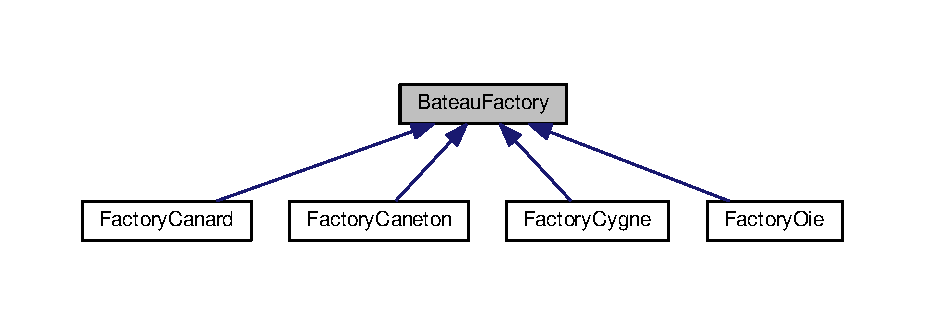
\includegraphics[width=350pt]{classBateauFactory__inherit__graph}
\end{center}
\end{figure}
\subsection*{Public Member Functions}
\begin{DoxyCompactItemize}
\item 
\hyperlink{classBateauFactory_ab2c99aa64b7804fa2d67699a2d80703a}{Bateau\+Factory} ()
\begin{DoxyCompactList}\small\item\em Constructeur. \end{DoxyCompactList}\item 
virtual std\+::shared\+\_\+ptr$<$ \hyperlink{classBateau}{Bateau} $>$ \hyperlink{classBateauFactory_a8cec9c2ab3793cec80e43b3d940da1d9}{creer\+Bateau} ()=0
\begin{DoxyCompactList}\small\item\em Récupère le \hyperlink{classBateau}{Bateau} créé \end{DoxyCompactList}\end{DoxyCompactItemize}


\subsection{Detailed Description}
classe representant un \char`\"{}\+Chantier Naval\char`\"{} 

La classe gère la création de Bateaux 

\subsection{Constructor \& Destructor Documentation}
\hypertarget{classBateauFactory_ab2c99aa64b7804fa2d67699a2d80703a}{\index{Bateau\+Factory@{Bateau\+Factory}!Bateau\+Factory@{Bateau\+Factory}}
\index{Bateau\+Factory@{Bateau\+Factory}!Bateau\+Factory@{Bateau\+Factory}}
\subsubsection[{Bateau\+Factory}]{\setlength{\rightskip}{0pt plus 5cm}Bateau\+Factory\+::\+Bateau\+Factory (
\begin{DoxyParamCaption}
{}
\end{DoxyParamCaption}
)}}\label{classBateauFactory_ab2c99aa64b7804fa2d67699a2d80703a}


Constructeur. 

Constructeur de la classe \hyperlink{classBateauFactory}{Bateau\+Factory} 

\subsection{Member Function Documentation}
\hypertarget{classBateauFactory_a8cec9c2ab3793cec80e43b3d940da1d9}{\index{Bateau\+Factory@{Bateau\+Factory}!creer\+Bateau@{creer\+Bateau}}
\index{creer\+Bateau@{creer\+Bateau}!Bateau\+Factory@{Bateau\+Factory}}
\subsubsection[{creer\+Bateau}]{\setlength{\rightskip}{0pt plus 5cm}virtual std\+::shared\+\_\+ptr$<${\bf Bateau}$>$ Bateau\+Factory\+::creer\+Bateau (
\begin{DoxyParamCaption}
{}
\end{DoxyParamCaption}
)\hspace{0.3cm}{\ttfamily [pure virtual]}}}\label{classBateauFactory_a8cec9c2ab3793cec80e43b3d940da1d9}


Récupère le \hyperlink{classBateau}{Bateau} créé 

Méthode permettant de récupérer le \hyperlink{classBateau}{Bateau} créé

\begin{DoxyReturn}{Returns}
le \hyperlink{classBateau}{Bateau} créé en fonction de la factory invoqué 
\end{DoxyReturn}


Implemented in \hyperlink{classFactoryCygne_aa49b4a3704bcb68c0e31cebc3f5767b8}{Factory\+Cygne}, \hyperlink{classFactoryCanard_a3ef0d9a9c293006fb09fd03a911a1377}{Factory\+Canard}, \hyperlink{classFactoryCaneton_ac03710919dab69d816bb4c8fd047f4eb}{Factory\+Caneton}, and \hyperlink{classFactoryOie_aef35f008954feedb26821fdf5b73328f}{Factory\+Oie}.



The documentation for this interface was generated from the following files\+:\begin{DoxyCompactItemize}
\item 
bateaufactory.\+h\item 
bateaufactory.\+cpp\end{DoxyCompactItemize}

\hypertarget{classCanard}{\section{Canard Class Reference}
\label{classCanard}\index{Canard@{Canard}}
}


classe representant un \hyperlink{classCanard}{Canard}  




{\ttfamily \#include $<$canard.\+h$>$}



Inheritance diagram for Canard\+:
\nopagebreak
\begin{figure}[H]
\begin{center}
\leavevmode
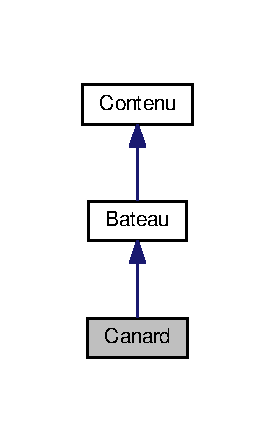
\includegraphics[width=132pt]{classCanard__inherit__graph}
\end{center}
\end{figure}


Collaboration diagram for Canard\+:
\nopagebreak
\begin{figure}[H]
\begin{center}
\leavevmode
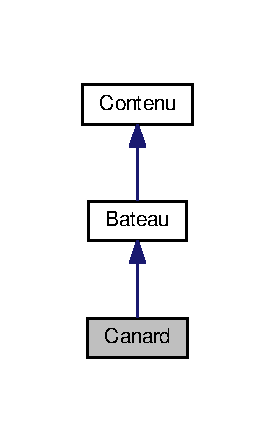
\includegraphics[width=132pt]{classCanard__coll__graph}
\end{center}
\end{figure}
\subsection*{Public Member Functions}
\begin{DoxyCompactItemize}
\item 
\hyperlink{classCanard_aca6cf94e49e14f5383fc7c798a8dfcf8}{Canard} ()
\begin{DoxyCompactList}\small\item\em Constructeur. \end{DoxyCompactList}\item 
int \hyperlink{classCanard_a5c99dcdcd79601f9cc075072c6fa8e47}{get\+Taille} ()
\begin{DoxyCompactList}\small\item\em Récupère la taille du \hyperlink{classBateau}{Bateau}. \end{DoxyCompactList}\end{DoxyCompactItemize}
\subsection*{Additional Inherited Members}


\subsection{Detailed Description}
classe representant un \hyperlink{classCanard}{Canard} 

La classe modélise un \hyperlink{classBateau}{Bateau} de taille 2 

\subsection{Constructor \& Destructor Documentation}
\hypertarget{classCanard_aca6cf94e49e14f5383fc7c798a8dfcf8}{\index{Canard@{Canard}!Canard@{Canard}}
\index{Canard@{Canard}!Canard@{Canard}}
\subsubsection[{Canard}]{\setlength{\rightskip}{0pt plus 5cm}Canard\+::\+Canard (
\begin{DoxyParamCaption}
{}
\end{DoxyParamCaption}
)}}\label{classCanard_aca6cf94e49e14f5383fc7c798a8dfcf8}


Constructeur. 

Constructeur de la classe \hyperlink{classCanard}{Canard} 

\subsection{Member Function Documentation}
\hypertarget{classCanard_a5c99dcdcd79601f9cc075072c6fa8e47}{\index{Canard@{Canard}!get\+Taille@{get\+Taille}}
\index{get\+Taille@{get\+Taille}!Canard@{Canard}}
\subsubsection[{get\+Taille}]{\setlength{\rightskip}{0pt plus 5cm}int Canard\+::get\+Taille (
\begin{DoxyParamCaption}
{}
\end{DoxyParamCaption}
)\hspace{0.3cm}{\ttfamily [virtual]}}}\label{classCanard_a5c99dcdcd79601f9cc075072c6fa8e47}


Récupère la taille du \hyperlink{classBateau}{Bateau}. 

Méthode permettant de récupérer la taille d'un \hyperlink{classCanard}{Canard}

\begin{DoxyReturn}{Returns}
la taille d'un \hyperlink{classCanard}{Canard} (2) 
\end{DoxyReturn}


Implements \hyperlink{classBateau_a08be20b8c871149d717a30b00c1068b9}{Bateau}.



The documentation for this class was generated from the following files\+:\begin{DoxyCompactItemize}
\item 
canard.\+h\item 
canard.\+cpp\end{DoxyCompactItemize}

\hypertarget{classCaneton}{\section{Caneton Class Reference}
\label{classCaneton}\index{Caneton@{Caneton}}
}


classe representant un \hyperlink{classCaneton}{Caneton}  




{\ttfamily \#include $<$caneton.\+h$>$}



Inheritance diagram for Caneton\+:
\nopagebreak
\begin{figure}[H]
\begin{center}
\leavevmode
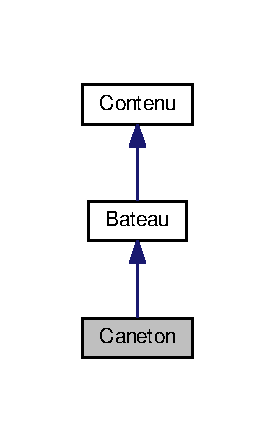
\includegraphics[width=132pt]{classCaneton__inherit__graph}
\end{center}
\end{figure}


Collaboration diagram for Caneton\+:
\nopagebreak
\begin{figure}[H]
\begin{center}
\leavevmode
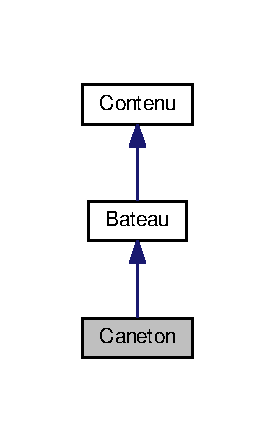
\includegraphics[width=132pt]{classCaneton__coll__graph}
\end{center}
\end{figure}
\subsection*{Public Member Functions}
\begin{DoxyCompactItemize}
\item 
\hyperlink{classCaneton_a8fecf932fc445c24b89c43342d5a4c36}{Caneton} ()
\begin{DoxyCompactList}\small\item\em Constructeur. \end{DoxyCompactList}\item 
int \hyperlink{classCaneton_a173cbd22638bbf2806a47c329284ceee}{get\+Taille} ()
\begin{DoxyCompactList}\small\item\em Récupère la taille du \hyperlink{classBateau}{Bateau}. \end{DoxyCompactList}\end{DoxyCompactItemize}
\subsection*{Additional Inherited Members}


\subsection{Detailed Description}
classe representant un \hyperlink{classCaneton}{Caneton} 

La classe modélise un \hyperlink{classBateau}{Bateau} de taille 1 

\subsection{Constructor \& Destructor Documentation}
\hypertarget{classCaneton_a8fecf932fc445c24b89c43342d5a4c36}{\index{Caneton@{Caneton}!Caneton@{Caneton}}
\index{Caneton@{Caneton}!Caneton@{Caneton}}
\subsubsection[{Caneton}]{\setlength{\rightskip}{0pt plus 5cm}Caneton\+::\+Caneton (
\begin{DoxyParamCaption}
{}
\end{DoxyParamCaption}
)}}\label{classCaneton_a8fecf932fc445c24b89c43342d5a4c36}


Constructeur. 

Constructeur de la classe \hyperlink{classCaneton}{Caneton} 

\subsection{Member Function Documentation}
\hypertarget{classCaneton_a173cbd22638bbf2806a47c329284ceee}{\index{Caneton@{Caneton}!get\+Taille@{get\+Taille}}
\index{get\+Taille@{get\+Taille}!Caneton@{Caneton}}
\subsubsection[{get\+Taille}]{\setlength{\rightskip}{0pt plus 5cm}int Caneton\+::get\+Taille (
\begin{DoxyParamCaption}
{}
\end{DoxyParamCaption}
)\hspace{0.3cm}{\ttfamily [virtual]}}}\label{classCaneton_a173cbd22638bbf2806a47c329284ceee}


Récupère la taille du \hyperlink{classBateau}{Bateau}. 

Méthode permettant de récupérer la taille d'un \hyperlink{classCaneton}{Caneton}

\begin{DoxyReturn}{Returns}
la taille d'un \hyperlink{classCaneton}{Caneton} (1) 
\end{DoxyReturn}


Implements \hyperlink{classBateau_a08be20b8c871149d717a30b00c1068b9}{Bateau}.



The documentation for this class was generated from the following files\+:\begin{DoxyCompactItemize}
\item 
caneton.\+h\item 
caneton.\+cpp\end{DoxyCompactItemize}

\hypertarget{classCarte}{\section{Carte Class Reference}
\label{classCarte}\index{Carte@{Carte}}
}


classe representant une \hyperlink{classCarte}{Carte}  




{\ttfamily \#include $<$carte.\+h$>$}



Inheritance diagram for Carte\+:
\nopagebreak
\begin{figure}[H]
\begin{center}
\leavevmode
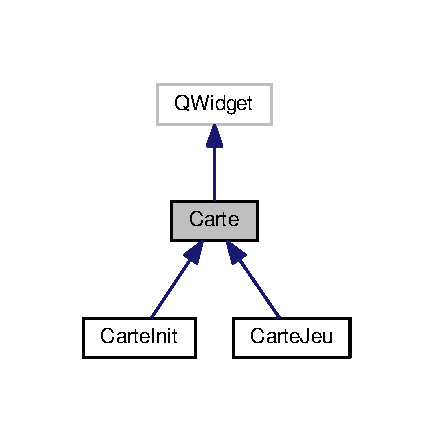
\includegraphics[width=208pt]{classCarte__inherit__graph}
\end{center}
\end{figure}


Collaboration diagram for Carte\+:
\nopagebreak
\begin{figure}[H]
\begin{center}
\leavevmode
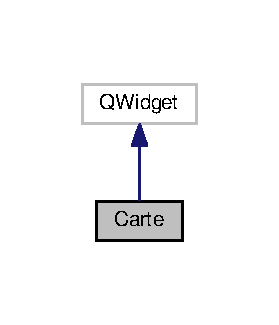
\includegraphics[width=134pt]{classCarte__coll__graph}
\end{center}
\end{figure}
\subsection*{Public Slots}
\begin{DoxyCompactItemize}
\item 
virtual void \hyperlink{classCarte_a8628e3d1c1c812b945f2cc3987ae1a40}{action\+Bouton} ()=0
\begin{DoxyCompactList}\small\item\em Action qui sera déclenché à chaque clic sur une case selon la carte (Init ou Jeu) \end{DoxyCompactList}\end{DoxyCompactItemize}
\subsection*{Public Member Functions}
\begin{DoxyCompactItemize}
\item 
\hyperlink{classCarte_a06daaca86c31c80f8308f4a81d46dc9b}{Carte} ()
\begin{DoxyCompactList}\small\item\em Constructeur. \end{DoxyCompactList}\item 
bool \hyperlink{classCarte_a8415ea8b3274e0fddecc122d83ce80a9}{ajouter\+Bateau} (std\+::shared\+\_\+ptr$<$ \hyperlink{classBateau}{Bateau} $>$ b)
\begin{DoxyCompactList}\small\item\em Ajout d'un \hyperlink{classBateau}{Bateau}. \end{DoxyCompactList}\item 
void \hyperlink{classCarte_ae4966ed5306a6f85453b556830935026}{enlever\+Bateau} (std\+::shared\+\_\+ptr$<$ \hyperlink{classBateau}{Bateau} $>$ b)
\begin{DoxyCompactList}\small\item\em Suppression d'un \hyperlink{classBateau}{Bateau}. \end{DoxyCompactList}\item 
Q\+Vector$<$ std\+::shared\+\_\+ptr\\*
$<$ \hyperlink{classBateau}{Bateau} $>$ $>$ \hyperlink{classCarte_ac05b028a316243ba5e66d4bfab48f6fa}{get\+Tab\+Bateau} ()
\begin{DoxyCompactList}\small\item\em Récupère l'ensemble des Bateaux de la carte. \end{DoxyCompactList}\item 
Q\+Vector$<$ \hyperlink{classCase}{Case} $\ast$ $>$ \hyperlink{classCarte_a6974f6c1fb5884205ba7b45f6ef7c89c}{get\+Tab\+Case} ()
\begin{DoxyCompactList}\small\item\em Récupère l'ensemble des \hyperlink{classCase}{Case} de la carte. \end{DoxyCompactList}\item 
void \hyperlink{classCarte_a108f801be6118ec28cf29102a68b4e9f}{reset} ()
\begin{DoxyCompactList}\small\item\em Remet à zéro la carte en enlevant tous les Bateaux. \end{DoxyCompactList}\end{DoxyCompactItemize}
\subsection*{Protected Attributes}
\begin{DoxyCompactItemize}
\item 
Q\+Vector$<$ \hyperlink{classCase}{Case} $\ast$ $>$ \hyperlink{classCarte_adb0cda59419437b3c29b4b6e7abbbbf5}{m\+\_\+tab\+Case}
\item 
Q\+Vector$<$ std\+::shared\+\_\+ptr\\*
$<$ \hyperlink{classBateau}{Bateau} $>$ $>$ \hyperlink{classCarte_a5551a4561583b6536efe31b8de645f60}{tab\+Bateaux\+\_\+}
\item 
Q\+Icon \hyperlink{classCarte_a8f5f0d81b5134126a52d338ea5d28dc6}{logo\+Case\+\_\+}
\item 
Q\+Pixmap \hyperlink{classCarte_a9077e065a5b672393b68afcbde4951f3}{cygne\+\_\+}
\item 
Q\+Pixmap \hyperlink{classCarte_ac66303b2e5f99770c450993f45b9ebc2}{oie\+\_\+}
\item 
Q\+Pixmap \hyperlink{classCarte_aaa54051f62acfe29059fb0973d977828}{canard\+\_\+}
\item 
Q\+Pixmap \hyperlink{classCarte_a824ab30e6ce53cc9c65c8af8146867f0}{caneton\+\_\+}
\item 
std\+::shared\+\_\+ptr$<$ \hyperlink{classBateauFactory}{Bateau\+Factory} $>$ \hyperlink{classCarte_afbc674d4d0a924d3a73c6f3f966a723a}{factory}
\end{DoxyCompactItemize}


\subsection{Detailed Description}
classe representant une \hyperlink{classCarte}{Carte} 

La classe modélise les actions que l'on peut faire sur une \hyperlink{classCarte}{Carte} 

\subsection{Constructor \& Destructor Documentation}
\hypertarget{classCarte_a06daaca86c31c80f8308f4a81d46dc9b}{\index{Carte@{Carte}!Carte@{Carte}}
\index{Carte@{Carte}!Carte@{Carte}}
\subsubsection[{Carte}]{\setlength{\rightskip}{0pt plus 5cm}Carte\+::\+Carte (
\begin{DoxyParamCaption}
{}
\end{DoxyParamCaption}
)}}\label{classCarte_a06daaca86c31c80f8308f4a81d46dc9b}


Constructeur. 

Constructeur de la classe \hyperlink{classCarte}{Carte} 

\subsection{Member Function Documentation}
\hypertarget{classCarte_a8628e3d1c1c812b945f2cc3987ae1a40}{\index{Carte@{Carte}!action\+Bouton@{action\+Bouton}}
\index{action\+Bouton@{action\+Bouton}!Carte@{Carte}}
\subsubsection[{action\+Bouton}]{\setlength{\rightskip}{0pt plus 5cm}virtual void Carte\+::action\+Bouton (
\begin{DoxyParamCaption}
{}
\end{DoxyParamCaption}
)\hspace{0.3cm}{\ttfamily [pure virtual]}, {\ttfamily [slot]}}}\label{classCarte_a8628e3d1c1c812b945f2cc3987ae1a40}


Action qui sera déclenché à chaque clic sur une case selon la carte (Init ou Jeu) 

Méthode permettant d'interagir lors du clic sur une case de la carte 

Implemented in \hyperlink{classCarteInit_a48844f800556030890bdc4d5933a3573}{Carte\+Init}, and \hyperlink{classCarteJeu_a9ba23d5a5b1e5d297c68ebd478f20a57}{Carte\+Jeu}.

\hypertarget{classCarte_a8415ea8b3274e0fddecc122d83ce80a9}{\index{Carte@{Carte}!ajouter\+Bateau@{ajouter\+Bateau}}
\index{ajouter\+Bateau@{ajouter\+Bateau}!Carte@{Carte}}
\subsubsection[{ajouter\+Bateau}]{\setlength{\rightskip}{0pt plus 5cm}bool Carte\+::ajouter\+Bateau (
\begin{DoxyParamCaption}
\item[{std\+::shared\+\_\+ptr$<$ {\bf Bateau} $>$}]{b}
\end{DoxyParamCaption}
)}}\label{classCarte_a8415ea8b3274e0fddecc122d83ce80a9}


Ajout d'un \hyperlink{classBateau}{Bateau}. 

Méthode permettant d'ajouter un \hyperlink{classBateau}{Bateau} sur la carte


\begin{DoxyParams}{Parameters}
{\em b} & \+: \hyperlink{classBateau}{Bateau} à ajouter\\
\hline
\end{DoxyParams}
\begin{DoxyReturn}{Returns}
true si le \hyperlink{classBateau}{Bateau} s'est placé sur la carte, sinon false 
\end{DoxyReturn}
\hypertarget{classCarte_ae4966ed5306a6f85453b556830935026}{\index{Carte@{Carte}!enlever\+Bateau@{enlever\+Bateau}}
\index{enlever\+Bateau@{enlever\+Bateau}!Carte@{Carte}}
\subsubsection[{enlever\+Bateau}]{\setlength{\rightskip}{0pt plus 5cm}void Carte\+::enlever\+Bateau (
\begin{DoxyParamCaption}
\item[{std\+::shared\+\_\+ptr$<$ {\bf Bateau} $>$}]{b}
\end{DoxyParamCaption}
)}}\label{classCarte_ae4966ed5306a6f85453b556830935026}


Suppression d'un \hyperlink{classBateau}{Bateau}. 

Méthode permettant de supprimer un \hyperlink{classBateau}{Bateau} sur la carte


\begin{DoxyParams}{Parameters}
{\em b} & \+: \hyperlink{classBateau}{Bateau} à supprimer \\
\hline
\end{DoxyParams}
\hypertarget{classCarte_ac05b028a316243ba5e66d4bfab48f6fa}{\index{Carte@{Carte}!get\+Tab\+Bateau@{get\+Tab\+Bateau}}
\index{get\+Tab\+Bateau@{get\+Tab\+Bateau}!Carte@{Carte}}
\subsubsection[{get\+Tab\+Bateau}]{\setlength{\rightskip}{0pt plus 5cm}Q\+Vector$<$ shared\+\_\+ptr$<$ {\bf Bateau} $>$ $>$ Carte\+::get\+Tab\+Bateau (
\begin{DoxyParamCaption}
{}
\end{DoxyParamCaption}
)}}\label{classCarte_ac05b028a316243ba5e66d4bfab48f6fa}


Récupère l'ensemble des Bateaux de la carte. 

Méthode permettant de récupérer l'ensemble des Bateaux qui ont été ajouté à la liste des Bateaux de la \hyperlink{classCarte}{Carte}

\begin{DoxyReturn}{Returns}
la liste des Bateaux qui ont été ajoutés à la carte 
\end{DoxyReturn}
\hypertarget{classCarte_a6974f6c1fb5884205ba7b45f6ef7c89c}{\index{Carte@{Carte}!get\+Tab\+Case@{get\+Tab\+Case}}
\index{get\+Tab\+Case@{get\+Tab\+Case}!Carte@{Carte}}
\subsubsection[{get\+Tab\+Case}]{\setlength{\rightskip}{0pt plus 5cm}Q\+Vector$<$ {\bf Case} $\ast$ $>$ Carte\+::get\+Tab\+Case (
\begin{DoxyParamCaption}
{}
\end{DoxyParamCaption}
)}}\label{classCarte_a6974f6c1fb5884205ba7b45f6ef7c89c}


Récupère l'ensemble des \hyperlink{classCase}{Case} de la carte. 

Méthode permettant de récupérer l'ensemble des 100 cases de la \hyperlink{classCarte}{Carte}

\begin{DoxyReturn}{Returns}
la liste des cases de la carte 
\end{DoxyReturn}
\hypertarget{classCarte_a108f801be6118ec28cf29102a68b4e9f}{\index{Carte@{Carte}!reset@{reset}}
\index{reset@{reset}!Carte@{Carte}}
\subsubsection[{reset}]{\setlength{\rightskip}{0pt plus 5cm}void Carte\+::reset (
\begin{DoxyParamCaption}
{}
\end{DoxyParamCaption}
)}}\label{classCarte_a108f801be6118ec28cf29102a68b4e9f}


Remet à zéro la carte en enlevant tous les Bateaux. 

Méthode permettant de supprimer tous les Bateaux déjà présents sur la carte en changeant le contenu de chaque case par de la \hyperlink{classMer}{Mer} 

\subsection{Member Data Documentation}
\hypertarget{classCarte_aaa54051f62acfe29059fb0973d977828}{\index{Carte@{Carte}!canard\+\_\+@{canard\+\_\+}}
\index{canard\+\_\+@{canard\+\_\+}!Carte@{Carte}}
\subsubsection[{canard\+\_\+}]{\setlength{\rightskip}{0pt plus 5cm}Q\+Pixmap Carte\+::canard\+\_\+\hspace{0.3cm}{\ttfamily [protected]}}}\label{classCarte_aaa54051f62acfe29059fb0973d977828}
image pour les bateaux de taille 2 \hypertarget{classCarte_a824ab30e6ce53cc9c65c8af8146867f0}{\index{Carte@{Carte}!caneton\+\_\+@{caneton\+\_\+}}
\index{caneton\+\_\+@{caneton\+\_\+}!Carte@{Carte}}
\subsubsection[{caneton\+\_\+}]{\setlength{\rightskip}{0pt plus 5cm}Q\+Pixmap Carte\+::caneton\+\_\+\hspace{0.3cm}{\ttfamily [protected]}}}\label{classCarte_a824ab30e6ce53cc9c65c8af8146867f0}
image pour les bateaux de taille 1 \hypertarget{classCarte_a9077e065a5b672393b68afcbde4951f3}{\index{Carte@{Carte}!cygne\+\_\+@{cygne\+\_\+}}
\index{cygne\+\_\+@{cygne\+\_\+}!Carte@{Carte}}
\subsubsection[{cygne\+\_\+}]{\setlength{\rightskip}{0pt plus 5cm}Q\+Pixmap Carte\+::cygne\+\_\+\hspace{0.3cm}{\ttfamily [protected]}}}\label{classCarte_a9077e065a5b672393b68afcbde4951f3}
image pour le bateau de taille 4 \hypertarget{classCarte_afbc674d4d0a924d3a73c6f3f966a723a}{\index{Carte@{Carte}!factory@{factory}}
\index{factory@{factory}!Carte@{Carte}}
\subsubsection[{factory}]{\setlength{\rightskip}{0pt plus 5cm}std\+::shared\+\_\+ptr$<${\bf Bateau\+Factory}$>$ Carte\+::factory\hspace{0.3cm}{\ttfamily [protected]}}}\label{classCarte_afbc674d4d0a924d3a73c6f3f966a723a}
le chantier naval pour la construction des bateaux \hypertarget{classCarte_a8f5f0d81b5134126a52d338ea5d28dc6}{\index{Carte@{Carte}!logo\+Case\+\_\+@{logo\+Case\+\_\+}}
\index{logo\+Case\+\_\+@{logo\+Case\+\_\+}!Carte@{Carte}}
\subsubsection[{logo\+Case\+\_\+}]{\setlength{\rightskip}{0pt plus 5cm}Q\+Icon Carte\+::logo\+Case\+\_\+\hspace{0.3cm}{\ttfamily [protected]}}}\label{classCarte_a8f5f0d81b5134126a52d338ea5d28dc6}
l'image que pourra prendre une case \hypertarget{classCarte_adb0cda59419437b3c29b4b6e7abbbbf5}{\index{Carte@{Carte}!m\+\_\+tab\+Case@{m\+\_\+tab\+Case}}
\index{m\+\_\+tab\+Case@{m\+\_\+tab\+Case}!Carte@{Carte}}
\subsubsection[{m\+\_\+tab\+Case}]{\setlength{\rightskip}{0pt plus 5cm}Q\+Vector$<${\bf Case}$\ast$$>$ Carte\+::m\+\_\+tab\+Case\hspace{0.3cm}{\ttfamily [protected]}}}\label{classCarte_adb0cda59419437b3c29b4b6e7abbbbf5}
liste des cases de la carte \hypertarget{classCarte_ac66303b2e5f99770c450993f45b9ebc2}{\index{Carte@{Carte}!oie\+\_\+@{oie\+\_\+}}
\index{oie\+\_\+@{oie\+\_\+}!Carte@{Carte}}
\subsubsection[{oie\+\_\+}]{\setlength{\rightskip}{0pt plus 5cm}Q\+Pixmap Carte\+::oie\+\_\+\hspace{0.3cm}{\ttfamily [protected]}}}\label{classCarte_ac66303b2e5f99770c450993f45b9ebc2}
image pour les bateaux de taille 3 \hypertarget{classCarte_a5551a4561583b6536efe31b8de645f60}{\index{Carte@{Carte}!tab\+Bateaux\+\_\+@{tab\+Bateaux\+\_\+}}
\index{tab\+Bateaux\+\_\+@{tab\+Bateaux\+\_\+}!Carte@{Carte}}
\subsubsection[{tab\+Bateaux\+\_\+}]{\setlength{\rightskip}{0pt plus 5cm}Q\+Vector$<$std\+::shared\+\_\+ptr$<${\bf Bateau}$>$ $>$ Carte\+::tab\+Bateaux\+\_\+\hspace{0.3cm}{\ttfamily [protected]}}}\label{classCarte_a5551a4561583b6536efe31b8de645f60}
liste des bateaux placés sur la carte 

The documentation for this class was generated from the following files\+:\begin{DoxyCompactItemize}
\item 
carte.\+h\item 
carte.\+cpp\end{DoxyCompactItemize}

\hypertarget{classCarteInit}{\section{Carte\+Init Class Reference}
\label{classCarteInit}\index{Carte\+Init@{Carte\+Init}}
}


classe representant une \hyperlink{classCarte}{Carte} d'initialisation  




{\ttfamily \#include $<$carteinit.\+h$>$}



Inheritance diagram for Carte\+Init\+:
\nopagebreak
\begin{figure}[H]
\begin{center}
\leavevmode
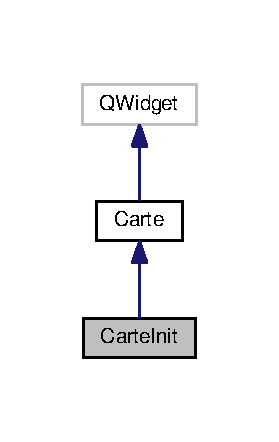
\includegraphics[width=134pt]{classCarteInit__inherit__graph}
\end{center}
\end{figure}


Collaboration diagram for Carte\+Init\+:
\nopagebreak
\begin{figure}[H]
\begin{center}
\leavevmode
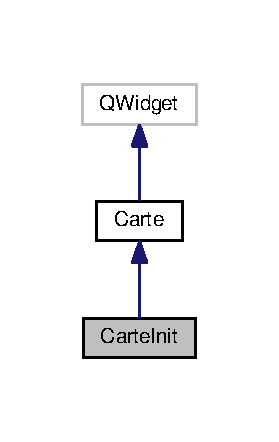
\includegraphics[width=134pt]{classCarteInit__coll__graph}
\end{center}
\end{figure}
\subsection*{Public Member Functions}
\begin{DoxyCompactItemize}
\item 
\hyperlink{classCarteInit_a54477b5d1d1662f277b70cb2d6efce27}{Carte\+Init} (std\+::shared\+\_\+ptr$<$ \hyperlink{classIAffichage}{I\+Affichage} $>$ a)
\begin{DoxyCompactList}\small\item\em Constructeur. \end{DoxyCompactList}\item 
\hyperlink{classCarteInit_a5e91e2c7caa1772484fb19aca3ba1a80}{Carte\+Init} (std\+::shared\+\_\+ptr$<$ \hyperlink{classAffichageInit}{Affichage\+Init} $>$ a)
\begin{DoxyCompactList}\small\item\em Constructeur. \end{DoxyCompactList}\item 
void \hyperlink{classCarteInit_a48844f800556030890bdc4d5933a3573}{action\+Bouton} ()
\begin{DoxyCompactList}\small\item\em Action qui sera déclenché à chaque clic sur une case. \end{DoxyCompactList}\end{DoxyCompactItemize}
\subsection*{Additional Inherited Members}


\subsection{Detailed Description}
classe representant une \hyperlink{classCarte}{Carte} d'initialisation 

La classe décrit ce qu'il est possible de faire avec une \hyperlink{classCarte}{Carte} d'initialisation 

\subsection{Constructor \& Destructor Documentation}
\hypertarget{classCarteInit_a54477b5d1d1662f277b70cb2d6efce27}{\index{Carte\+Init@{Carte\+Init}!Carte\+Init@{Carte\+Init}}
\index{Carte\+Init@{Carte\+Init}!Carte\+Init@{Carte\+Init}}
\subsubsection[{Carte\+Init}]{\setlength{\rightskip}{0pt plus 5cm}Carte\+Init\+::\+Carte\+Init (
\begin{DoxyParamCaption}
\item[{std\+::shared\+\_\+ptr$<$ {\bf I\+Affichage} $>$}]{a}
\end{DoxyParamCaption}
)}}\label{classCarteInit_a54477b5d1d1662f277b70cb2d6efce27}


Constructeur. 

Constructeur de la classe \hyperlink{classCarteInit}{Carte\+Init}


\begin{DoxyParams}{Parameters}
{\em a} & \+: le paramètre est un \hyperlink{classIAffichage}{I\+Affichage} en cas de besoin \\
\hline
\end{DoxyParams}
\hypertarget{classCarteInit_a5e91e2c7caa1772484fb19aca3ba1a80}{\index{Carte\+Init@{Carte\+Init}!Carte\+Init@{Carte\+Init}}
\index{Carte\+Init@{Carte\+Init}!Carte\+Init@{Carte\+Init}}
\subsubsection[{Carte\+Init}]{\setlength{\rightskip}{0pt plus 5cm}Carte\+Init\+::\+Carte\+Init (
\begin{DoxyParamCaption}
\item[{std\+::shared\+\_\+ptr$<$ {\bf Affichage\+Init} $>$}]{a}
\end{DoxyParamCaption}
)}}\label{classCarteInit_a5e91e2c7caa1772484fb19aca3ba1a80}


Constructeur. 

Constructeur de la classe \hyperlink{classCarteInit}{Carte\+Init}


\begin{DoxyParams}{Parameters}
{\em a} & \+: le paramètre est un \hyperlink{classAffichageInit}{Affichage\+Init} en cas de besoin \\
\hline
\end{DoxyParams}


\subsection{Member Function Documentation}
\hypertarget{classCarteInit_a48844f800556030890bdc4d5933a3573}{\index{Carte\+Init@{Carte\+Init}!action\+Bouton@{action\+Bouton}}
\index{action\+Bouton@{action\+Bouton}!Carte\+Init@{Carte\+Init}}
\subsubsection[{action\+Bouton}]{\setlength{\rightskip}{0pt plus 5cm}void Carte\+Init\+::action\+Bouton (
\begin{DoxyParamCaption}
{}
\end{DoxyParamCaption}
)\hspace{0.3cm}{\ttfamily [virtual]}}}\label{classCarteInit_a48844f800556030890bdc4d5933a3573}


Action qui sera déclenché à chaque clic sur une case. 

Méthode permettant d'interagir lors du clic sur une case de la carte 

Implements \hyperlink{classCarte_a8628e3d1c1c812b945f2cc3987ae1a40}{Carte}.



The documentation for this class was generated from the following files\+:\begin{DoxyCompactItemize}
\item 
carteinit.\+h\item 
carteinit.\+cpp\end{DoxyCompactItemize}

\hypertarget{classCarteJeu}{\section{Carte\+Jeu Class Reference}
\label{classCarteJeu}\index{Carte\+Jeu@{Carte\+Jeu}}
}


classe representant une \hyperlink{classCarte}{Carte} de jeu  




{\ttfamily \#include $<$cartejeu.\+h$>$}



Inheritance diagram for Carte\+Jeu\+:
\nopagebreak
\begin{figure}[H]
\begin{center}
\leavevmode
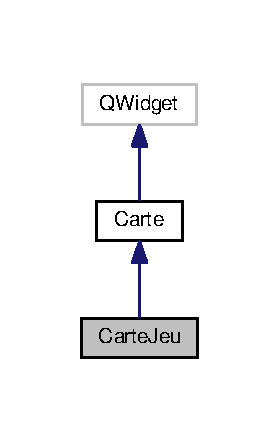
\includegraphics[width=134pt]{classCarteJeu__inherit__graph}
\end{center}
\end{figure}


Collaboration diagram for Carte\+Jeu\+:
\nopagebreak
\begin{figure}[H]
\begin{center}
\leavevmode
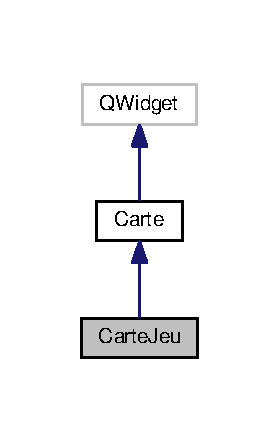
\includegraphics[width=134pt]{classCarteJeu__coll__graph}
\end{center}
\end{figure}
\subsection*{Public Member Functions}
\begin{DoxyCompactItemize}
\item 
\hyperlink{classCarteJeu_a5c18cd639d1e3f69acb77056623fcb9a}{Carte\+Jeu} (\hyperlink{classAffichageJeu}{Affichage\+Jeu} $\ast$a)
\begin{DoxyCompactList}\small\item\em Constructeur. \end{DoxyCompactList}\item 
void \hyperlink{classCarteJeu_a9ba23d5a5b1e5d297c68ebd478f20a57}{action\+Bouton} ()
\begin{DoxyCompactList}\small\item\em Action qui sera déclenché à chaque clic sur une case. \end{DoxyCompactList}\end{DoxyCompactItemize}
\subsection*{Additional Inherited Members}


\subsection{Detailed Description}
classe representant une \hyperlink{classCarte}{Carte} de jeu 

La classe décrit ce qu'il est possible de faire avec une \hyperlink{classCarte}{Carte} d'initialisation 

\subsection{Constructor \& Destructor Documentation}
\hypertarget{classCarteJeu_a5c18cd639d1e3f69acb77056623fcb9a}{\index{Carte\+Jeu@{Carte\+Jeu}!Carte\+Jeu@{Carte\+Jeu}}
\index{Carte\+Jeu@{Carte\+Jeu}!Carte\+Jeu@{Carte\+Jeu}}
\subsubsection[{Carte\+Jeu}]{\setlength{\rightskip}{0pt plus 5cm}Carte\+Jeu\+::\+Carte\+Jeu (
\begin{DoxyParamCaption}
\item[{{\bf Affichage\+Jeu} $\ast$}]{a}
\end{DoxyParamCaption}
)}}\label{classCarteJeu_a5c18cd639d1e3f69acb77056623fcb9a}


Constructeur. 

Constructeur de la classe \hyperlink{classCarteJeu}{Carte\+Jeu}


\begin{DoxyParams}{Parameters}
{\em a} & \+: le paramètre est un \hyperlink{classAffichageJeu}{Affichage\+Jeu} en cas de besoin \\
\hline
\end{DoxyParams}


\subsection{Member Function Documentation}
\hypertarget{classCarteJeu_a9ba23d5a5b1e5d297c68ebd478f20a57}{\index{Carte\+Jeu@{Carte\+Jeu}!action\+Bouton@{action\+Bouton}}
\index{action\+Bouton@{action\+Bouton}!Carte\+Jeu@{Carte\+Jeu}}
\subsubsection[{action\+Bouton}]{\setlength{\rightskip}{0pt plus 5cm}void Carte\+Jeu\+::action\+Bouton (
\begin{DoxyParamCaption}
{}
\end{DoxyParamCaption}
)\hspace{0.3cm}{\ttfamily [virtual]}}}\label{classCarteJeu_a9ba23d5a5b1e5d297c68ebd478f20a57}


Action qui sera déclenché à chaque clic sur une case. 

Méthode permettant d'interagir lors du clic sur une case de la carte 

Implements \hyperlink{classCarte_a8628e3d1c1c812b945f2cc3987ae1a40}{Carte}.



The documentation for this class was generated from the following files\+:\begin{DoxyCompactItemize}
\item 
cartejeu.\+h\item 
cartejeu.\+cpp\end{DoxyCompactItemize}

\hypertarget{classCase}{\section{Case Class Reference}
\label{classCase}\index{Case@{Case}}
}


classe representant une \hyperlink{classCase}{Case}  




{\ttfamily \#include $<$case.\+h$>$}



Inheritance diagram for Case\+:
\nopagebreak
\begin{figure}[H]
\begin{center}
\leavevmode
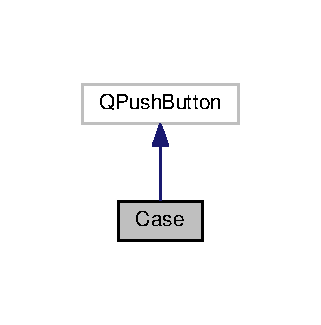
\includegraphics[width=154pt]{classCase__inherit__graph}
\end{center}
\end{figure}


Collaboration diagram for Case\+:
\nopagebreak
\begin{figure}[H]
\begin{center}
\leavevmode
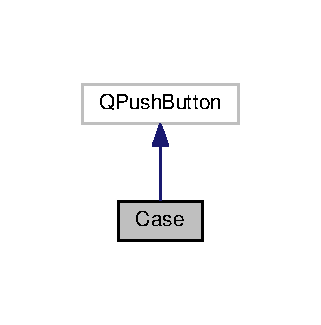
\includegraphics[width=154pt]{classCase__coll__graph}
\end{center}
\end{figure}
\subsection*{Public Member Functions}
\begin{DoxyCompactItemize}
\item 
\hyperlink{classCase_a5fc4408a8eea8e390fd9b8d3ae6345a7}{Case} (Q\+Widget $\ast$parent, int x, int y)
\begin{DoxyCompactList}\small\item\em Constructeur. \end{DoxyCompactList}\item 
bool \hyperlink{classCase_afa446bb3223628f76144f077df5e7618}{clic} ()
\begin{DoxyCompactList}\small\item\em Permet de savoir si la case a déjà été touchée et ce qu'elle contient. \end{DoxyCompactList}\item 
int \hyperlink{classCase_ab5580b919199dd2ec379672d3390bbff}{get\+X} ()
\begin{DoxyCompactList}\small\item\em Récupère la ligne où se trouve la case. \end{DoxyCompactList}\item 
int \hyperlink{classCase_a824f612c5a660a1d55ac06931747c46d}{get\+Y} ()
\begin{DoxyCompactList}\small\item\em Récupère la colonne où se trouve la case. \end{DoxyCompactList}\item 
void \hyperlink{classCase_a77e28934961e13da9fcf0f1168b8e7a4}{to\+String} ()
\begin{DoxyCompactList}\small\item\em Décrit la case. \end{DoxyCompactList}\item 
std\+::shared\+\_\+ptr$<$ \hyperlink{classContenu}{Contenu} $>$ \hyperlink{classCase_ae761fa055a6c3e3e228d22b503b525ae}{get\+Content} ()
\begin{DoxyCompactList}\small\item\em Récupère le contenu de la case. \end{DoxyCompactList}\item 
void \hyperlink{classCase_a474429530bc089e09a51410ca92a5ad7}{set\+Content} (\hyperlink{classContenu}{Contenu} $\ast$c)
\begin{DoxyCompactList}\small\item\em Modifie le contenu de la case. \end{DoxyCompactList}\item 
void \hyperlink{classCase_ae461d39a197ed070e54f430c681b93b1}{set\+Content} (std\+::shared\+\_\+ptr$<$ \hyperlink{classContenu}{Contenu} $>$ c)
\begin{DoxyCompactList}\small\item\em Modifie le contenu de la case. \end{DoxyCompactList}\item 
bool \hyperlink{classCase_ae66f6f25dbb860d02ee3a7af62fc56eb}{is\+Empty} ()
\begin{DoxyCompactList}\small\item\em Savoir si le contenu de la case est vide (de la \hyperlink{classMer}{Mer}) \end{DoxyCompactList}\item 
void \hyperlink{classCase_abc8ddec34f7f32980b8c2af01934a45a}{reset\+Case} ()
\begin{DoxyCompactList}\small\item\em Permet de vider la case. \end{DoxyCompactList}\item 
\hypertarget{classCase_ab004564aae3e15db0c7fd5dde0b4c379}{virtual \hyperlink{classCase_ab004564aae3e15db0c7fd5dde0b4c379}{$\sim$\+Case} ()}\label{classCase_ab004564aae3e15db0c7fd5dde0b4c379}

\begin{DoxyCompactList}\small\item\em Destructeur Destructeur de la classe \hyperlink{classCase}{Case}. \end{DoxyCompactList}\end{DoxyCompactItemize}


\subsection{Detailed Description}
classe representant une \hyperlink{classCase}{Case} 

La classe décrit une case qui composera une carte 

\subsection{Constructor \& Destructor Documentation}
\hypertarget{classCase_a5fc4408a8eea8e390fd9b8d3ae6345a7}{\index{Case@{Case}!Case@{Case}}
\index{Case@{Case}!Case@{Case}}
\subsubsection[{Case}]{\setlength{\rightskip}{0pt plus 5cm}Case\+::\+Case (
\begin{DoxyParamCaption}
\item[{Q\+Widget $\ast$}]{parent, }
\item[{int}]{x, }
\item[{int}]{y}
\end{DoxyParamCaption}
)}}\label{classCase_a5fc4408a8eea8e390fd9b8d3ae6345a7}


Constructeur. 

Constructeur de la classe \hyperlink{classCase}{Case}


\begin{DoxyParams}{Parameters}
{\em parent} & \+: déigne le parent de la case (la carte) \\
\hline
{\em x} & \+: le numéro de ligne de la case \\
\hline
{\em y} & \+: le numéro de colonne de la case \\
\hline
\end{DoxyParams}


\subsection{Member Function Documentation}
\hypertarget{classCase_afa446bb3223628f76144f077df5e7618}{\index{Case@{Case}!clic@{clic}}
\index{clic@{clic}!Case@{Case}}
\subsubsection[{clic}]{\setlength{\rightskip}{0pt plus 5cm}bool Case\+::clic (
\begin{DoxyParamCaption}
{}
\end{DoxyParamCaption}
)}}\label{classCase_afa446bb3223628f76144f077df5e7618}


Permet de savoir si la case a déjà été touchée et ce qu'elle contient. 

Méthode permettant de savoir si la case a déjà été cliqué et connaitre son contenu grâce à son retour

\begin{DoxyReturn}{Returns}
true si la case a déjà été touchée ou s'il s'agit d'un bateau, sinon false 
\end{DoxyReturn}
\hypertarget{classCase_ae761fa055a6c3e3e228d22b503b525ae}{\index{Case@{Case}!get\+Content@{get\+Content}}
\index{get\+Content@{get\+Content}!Case@{Case}}
\subsubsection[{get\+Content}]{\setlength{\rightskip}{0pt plus 5cm}shared\+\_\+ptr$<$ {\bf Contenu} $>$ Case\+::get\+Content (
\begin{DoxyParamCaption}
{}
\end{DoxyParamCaption}
)}}\label{classCase_ae761fa055a6c3e3e228d22b503b525ae}


Récupère le contenu de la case. 

Méthode permettant de récupérer le contenu de la case

\begin{DoxyReturn}{Returns}
le contenu la case (\hyperlink{classBateau}{Bateau} ou \hyperlink{classMer}{Mer}) 
\end{DoxyReturn}
\hypertarget{classCase_ab5580b919199dd2ec379672d3390bbff}{\index{Case@{Case}!get\+X@{get\+X}}
\index{get\+X@{get\+X}!Case@{Case}}
\subsubsection[{get\+X}]{\setlength{\rightskip}{0pt plus 5cm}int Case\+::get\+X (
\begin{DoxyParamCaption}
{}
\end{DoxyParamCaption}
)}}\label{classCase_ab5580b919199dd2ec379672d3390bbff}


Récupère la ligne où se trouve la case. 

Méthode permettant de récupérer la ligne sur laquelle se situe la case sur la carte

\begin{DoxyReturn}{Returns}
le numéro de ligne sur laquelle se trouve la case 
\end{DoxyReturn}
\hypertarget{classCase_a824f612c5a660a1d55ac06931747c46d}{\index{Case@{Case}!get\+Y@{get\+Y}}
\index{get\+Y@{get\+Y}!Case@{Case}}
\subsubsection[{get\+Y}]{\setlength{\rightskip}{0pt plus 5cm}int Case\+::get\+Y (
\begin{DoxyParamCaption}
{}
\end{DoxyParamCaption}
)}}\label{classCase_a824f612c5a660a1d55ac06931747c46d}


Récupère la colonne où se trouve la case. 

Méthode permettant de récupérer la colonne sur laquelle se situe la case sur la carte

\begin{DoxyReturn}{Returns}
le numéro de colonne sur laquelle se trouve la case 
\end{DoxyReturn}
\hypertarget{classCase_ae66f6f25dbb860d02ee3a7af62fc56eb}{\index{Case@{Case}!is\+Empty@{is\+Empty}}
\index{is\+Empty@{is\+Empty}!Case@{Case}}
\subsubsection[{is\+Empty}]{\setlength{\rightskip}{0pt plus 5cm}bool Case\+::is\+Empty (
\begin{DoxyParamCaption}
{}
\end{DoxyParamCaption}
)}}\label{classCase_ae66f6f25dbb860d02ee3a7af62fc56eb}


Savoir si le contenu de la case est vide (de la \hyperlink{classMer}{Mer}) 

Méthode permettant de savoir si le contenu de la case est de la \hyperlink{classMer}{Mer} ou non

\begin{DoxyReturn}{Returns}
true si le contenu de la case est de la \hyperlink{classMer}{Mer}, sinon false 
\end{DoxyReturn}
\hypertarget{classCase_abc8ddec34f7f32980b8c2af01934a45a}{\index{Case@{Case}!reset\+Case@{reset\+Case}}
\index{reset\+Case@{reset\+Case}!Case@{Case}}
\subsubsection[{reset\+Case}]{\setlength{\rightskip}{0pt plus 5cm}void Case\+::reset\+Case (
\begin{DoxyParamCaption}
{}
\end{DoxyParamCaption}
)}}\label{classCase_abc8ddec34f7f32980b8c2af01934a45a}


Permet de vider la case. 

Méthode permettant de modifier le contenu de la case par de la \hyperlink{classMer}{Mer} \hypertarget{classCase_a474429530bc089e09a51410ca92a5ad7}{\index{Case@{Case}!set\+Content@{set\+Content}}
\index{set\+Content@{set\+Content}!Case@{Case}}
\subsubsection[{set\+Content}]{\setlength{\rightskip}{0pt plus 5cm}void Case\+::set\+Content (
\begin{DoxyParamCaption}
\item[{{\bf Contenu} $\ast$}]{c}
\end{DoxyParamCaption}
)}}\label{classCase_a474429530bc089e09a51410ca92a5ad7}


Modifie le contenu de la case. 

Méthode permettant modifier le contenu de la case


\begin{DoxyParams}{Parameters}
{\em c} & \+: le nouveau contenu de la case (\hyperlink{classMer}{Mer} ou \hyperlink{classBateau}{Bateau}) \\
\hline
\end{DoxyParams}
\hypertarget{classCase_ae461d39a197ed070e54f430c681b93b1}{\index{Case@{Case}!set\+Content@{set\+Content}}
\index{set\+Content@{set\+Content}!Case@{Case}}
\subsubsection[{set\+Content}]{\setlength{\rightskip}{0pt plus 5cm}void Case\+::set\+Content (
\begin{DoxyParamCaption}
\item[{std\+::shared\+\_\+ptr$<$ {\bf Contenu} $>$}]{c}
\end{DoxyParamCaption}
)}}\label{classCase_ae461d39a197ed070e54f430c681b93b1}


Modifie le contenu de la case. 

Méthode permettant modifier le contenu de la case


\begin{DoxyParams}{Parameters}
{\em c} & \+: le nouveau contenu de la case (\hyperlink{classMer}{Mer} ou \hyperlink{classBateau}{Bateau}) \\
\hline
\end{DoxyParams}
\hypertarget{classCase_a77e28934961e13da9fcf0f1168b8e7a4}{\index{Case@{Case}!to\+String@{to\+String}}
\index{to\+String@{to\+String}!Case@{Case}}
\subsubsection[{to\+String}]{\setlength{\rightskip}{0pt plus 5cm}void Case\+::to\+String (
\begin{DoxyParamCaption}
{}
\end{DoxyParamCaption}
)}}\label{classCase_a77e28934961e13da9fcf0f1168b8e7a4}


Décrit la case. 

Méthode permettant de décrire la case avec ses coordonnées 

The documentation for this class was generated from the following files\+:\begin{DoxyCompactItemize}
\item 
case.\+h\item 
case.\+cpp\end{DoxyCompactItemize}

\hypertarget{classCompMode}{\section{Comp\+Mode Class Reference}
\label{classCompMode}\index{Comp\+Mode@{Comp\+Mode}}
}


classe representant un comportement de mode de jeu  




{\ttfamily \#include $<$compmode.\+h$>$}



Inheritance diagram for Comp\+Mode\+:
\nopagebreak
\begin{figure}[H]
\begin{center}
\leavevmode
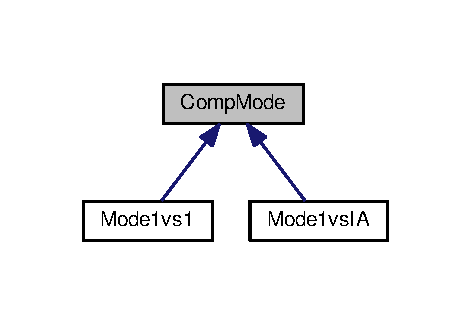
\includegraphics[width=226pt]{classCompMode__inherit__graph}
\end{center}
\end{figure}
\subsection*{Public Member Functions}
\begin{DoxyCompactItemize}
\item 
\hyperlink{classCompMode_aab4f503377e812cd05e2f1914c2faae3}{Comp\+Mode} ()
\begin{DoxyCompactList}\small\item\em Constructeur. \end{DoxyCompactList}\item 
virtual void \hyperlink{classCompMode_a897f6f474d86453c91ab83ab61c6f031}{get\+Mode} ()=0
\begin{DoxyCompactList}\small\item\em Décrit le mode dans lequel on est. \end{DoxyCompactList}\item 
virtual void \hyperlink{classCompMode_a3559cd952b7f3c6f8e7f22f6f3dc23ae}{initialiser} ()=0
\begin{DoxyCompactList}\small\item\em Initialiser la carte d'initialisation. \end{DoxyCompactList}\item 
virtual void \hyperlink{classCompMode_a1e3c25af2e4e655d8ab55b77854069d7}{fin\+Init\+J1} ()=0
\begin{DoxyCompactList}\small\item\em Indiquer lorsque le J1 a fini d'initialiser sa carte. \end{DoxyCompactList}\item 
virtual void \hyperlink{classCompMode_a311cf95ec88795dfb14dbed569a7d54f}{lancer} ()=0
\begin{DoxyCompactList}\small\item\em Indiquer lorsque le J2 a fini d'initialiser sa carte. \end{DoxyCompactList}\item 
virtual void \hyperlink{classCompMode_a81615504b7d72e0255b7fc09a991e0b5}{jouer} ()=0
\begin{DoxyCompactList}\small\item\em Jouer selon le mode de jeu. \end{DoxyCompactList}\item 
virtual void \hyperlink{classCompMode_a6b26d4c754fe0cc104d24d79f472b24d}{touche} ()=0
\begin{DoxyCompactList}\small\item\em Action produit après avoir touché un bateau. \end{DoxyCompactList}\item 
virtual void \hyperlink{classCompMode_a94119b30f5d6704464023e97b5656e9d}{set\+Affichage} (std\+::shared\+\_\+ptr$<$ \hyperlink{classIAffichage}{I\+Affichage} $>$ aff)=0
\begin{DoxyCompactList}\small\item\em Permet de changer l'affichage actif. \end{DoxyCompactList}\item 
virtual void \hyperlink{classCompMode_a537f7077c642a62627ab008bc85642df}{choix\+Pour\+J2} ()=0
\begin{DoxyCompactList}\small\item\em Action produit pour le J2. \end{DoxyCompactList}\item 
\hypertarget{classCompMode_ab18f0c9871e896d55e6b85eb8a77203d}{virtual \hyperlink{classCompMode_ab18f0c9871e896d55e6b85eb8a77203d}{$\sim$\+Comp\+Mode} ()}\label{classCompMode_ab18f0c9871e896d55e6b85eb8a77203d}

\begin{DoxyCompactList}\small\item\em Destructeur Destructeur de la classe \hyperlink{classCompMode}{Comp\+Mode}. \end{DoxyCompactList}\end{DoxyCompactItemize}
\subsection*{Protected Attributes}
\begin{DoxyCompactItemize}
\item 
std\+::shared\+\_\+ptr$<$ \hyperlink{classIAffichage}{I\+Affichage} $>$ \hyperlink{classCompMode_abb71bc830a23d19f68c821f4d1564488}{aff\+\_\+}
\end{DoxyCompactItemize}


\subsection{Detailed Description}
classe representant un comportement de mode de jeu 

La classe décrit les actions possibles dans les comportements de mode 

\subsection{Constructor \& Destructor Documentation}
\hypertarget{classCompMode_aab4f503377e812cd05e2f1914c2faae3}{\index{Comp\+Mode@{Comp\+Mode}!Comp\+Mode@{Comp\+Mode}}
\index{Comp\+Mode@{Comp\+Mode}!Comp\+Mode@{Comp\+Mode}}
\subsubsection[{Comp\+Mode}]{\setlength{\rightskip}{0pt plus 5cm}Comp\+Mode\+::\+Comp\+Mode (
\begin{DoxyParamCaption}
{}
\end{DoxyParamCaption}
)}}\label{classCompMode_aab4f503377e812cd05e2f1914c2faae3}


Constructeur. 

Constructeur de la classe \hyperlink{classCompMode}{Comp\+Mode} 

\subsection{Member Function Documentation}
\hypertarget{classCompMode_a537f7077c642a62627ab008bc85642df}{\index{Comp\+Mode@{Comp\+Mode}!choix\+Pour\+J2@{choix\+Pour\+J2}}
\index{choix\+Pour\+J2@{choix\+Pour\+J2}!Comp\+Mode@{Comp\+Mode}}
\subsubsection[{choix\+Pour\+J2}]{\setlength{\rightskip}{0pt plus 5cm}virtual void Comp\+Mode\+::choix\+Pour\+J2 (
\begin{DoxyParamCaption}
{}
\end{DoxyParamCaption}
)\hspace{0.3cm}{\ttfamily [pure virtual]}}}\label{classCompMode_a537f7077c642a62627ab008bc85642df}


Action produit pour le J2. 

Méthode permettant de choisir l'action à effectuer pour le J2 

Implemented in \hyperlink{classMode1vsIA_a3dce01c56c0c5008f0e7a4dcb4d9834a}{Mode1vs\+I\+A}, and \hyperlink{classMode1vs1_a031055c6d9efcc1dd3249c9396f9b496}{Mode1vs1}.

\hypertarget{classCompMode_a1e3c25af2e4e655d8ab55b77854069d7}{\index{Comp\+Mode@{Comp\+Mode}!fin\+Init\+J1@{fin\+Init\+J1}}
\index{fin\+Init\+J1@{fin\+Init\+J1}!Comp\+Mode@{Comp\+Mode}}
\subsubsection[{fin\+Init\+J1}]{\setlength{\rightskip}{0pt plus 5cm}virtual void Comp\+Mode\+::fin\+Init\+J1 (
\begin{DoxyParamCaption}
{}
\end{DoxyParamCaption}
)\hspace{0.3cm}{\ttfamily [pure virtual]}}}\label{classCompMode_a1e3c25af2e4e655d8ab55b77854069d7}


Indiquer lorsque le J1 a fini d'initialiser sa carte. 

Méthode permettant de passer à la phase d'initialisation pour le J2 

Implemented in \hyperlink{classMode1vsIA_ab50fb645a214d5cfab5fdb7a2b98673c}{Mode1vs\+I\+A}, and \hyperlink{classMode1vs1_a21a9f0c6705700943538ce86ec252ad6}{Mode1vs1}.

\hypertarget{classCompMode_a897f6f474d86453c91ab83ab61c6f031}{\index{Comp\+Mode@{Comp\+Mode}!get\+Mode@{get\+Mode}}
\index{get\+Mode@{get\+Mode}!Comp\+Mode@{Comp\+Mode}}
\subsubsection[{get\+Mode}]{\setlength{\rightskip}{0pt plus 5cm}virtual void Comp\+Mode\+::get\+Mode (
\begin{DoxyParamCaption}
{}
\end{DoxyParamCaption}
)\hspace{0.3cm}{\ttfamily [pure virtual]}}}\label{classCompMode_a897f6f474d86453c91ab83ab61c6f031}


Décrit le mode dans lequel on est. 

Méthode permettant décrire le mode 1\+V1 ou 1\+V\+I\+A 

Implemented in \hyperlink{classMode1vsIA_a8853a5c4bd43685f2232929f9d9d8732}{Mode1vs\+I\+A}, and \hyperlink{classMode1vs1_a7e38b115b83c63fe95a0fd96594c6fd9}{Mode1vs1}.

\hypertarget{classCompMode_a3559cd952b7f3c6f8e7f22f6f3dc23ae}{\index{Comp\+Mode@{Comp\+Mode}!initialiser@{initialiser}}
\index{initialiser@{initialiser}!Comp\+Mode@{Comp\+Mode}}
\subsubsection[{initialiser}]{\setlength{\rightskip}{0pt plus 5cm}virtual void Comp\+Mode\+::initialiser (
\begin{DoxyParamCaption}
{}
\end{DoxyParamCaption}
)\hspace{0.3cm}{\ttfamily [pure virtual]}}}\label{classCompMode_a3559cd952b7f3c6f8e7f22f6f3dc23ae}


Initialiser la carte d'initialisation. 

Méthode permettant d'initialiser la carte (pour l'I\+A) 

Implemented in \hyperlink{classMode1vsIA_a2e92031d0b7626da4f87ecc856a4ae94}{Mode1vs\+I\+A}, and \hyperlink{classMode1vs1_a96b5ffac518dc015717e361248715e78}{Mode1vs1}.

\hypertarget{classCompMode_a81615504b7d72e0255b7fc09a991e0b5}{\index{Comp\+Mode@{Comp\+Mode}!jouer@{jouer}}
\index{jouer@{jouer}!Comp\+Mode@{Comp\+Mode}}
\subsubsection[{jouer}]{\setlength{\rightskip}{0pt plus 5cm}virtual void Comp\+Mode\+::jouer (
\begin{DoxyParamCaption}
{}
\end{DoxyParamCaption}
)\hspace{0.3cm}{\ttfamily [pure virtual]}}}\label{classCompMode_a81615504b7d72e0255b7fc09a991e0b5}


Jouer selon le mode de jeu. 

Méthode permettant de décrire les actions produits pendant un tour de jeu 

Implemented in \hyperlink{classMode1vsIA_a7f7ab3fae5995ab12d6ce508c3d7dbca}{Mode1vs\+I\+A}, and \hyperlink{classMode1vs1_ac79db87b0b4a3c72ebf6300ed708c40d}{Mode1vs1}.

\hypertarget{classCompMode_a311cf95ec88795dfb14dbed569a7d54f}{\index{Comp\+Mode@{Comp\+Mode}!lancer@{lancer}}
\index{lancer@{lancer}!Comp\+Mode@{Comp\+Mode}}
\subsubsection[{lancer}]{\setlength{\rightskip}{0pt plus 5cm}virtual void Comp\+Mode\+::lancer (
\begin{DoxyParamCaption}
{}
\end{DoxyParamCaption}
)\hspace{0.3cm}{\ttfamily [pure virtual]}}}\label{classCompMode_a311cf95ec88795dfb14dbed569a7d54f}


Indiquer lorsque le J2 a fini d'initialiser sa carte. 

Méthode permettant de passer à la phase de jeu 

Implemented in \hyperlink{classMode1vsIA_ab6aa884defaf26231ede82d689b80d60}{Mode1vs\+I\+A}, and \hyperlink{classMode1vs1_a4b62821aec55d3a01257eb9cf3d4fd28}{Mode1vs1}.

\hypertarget{classCompMode_a94119b30f5d6704464023e97b5656e9d}{\index{Comp\+Mode@{Comp\+Mode}!set\+Affichage@{set\+Affichage}}
\index{set\+Affichage@{set\+Affichage}!Comp\+Mode@{Comp\+Mode}}
\subsubsection[{set\+Affichage}]{\setlength{\rightskip}{0pt plus 5cm}virtual void Comp\+Mode\+::set\+Affichage (
\begin{DoxyParamCaption}
\item[{std\+::shared\+\_\+ptr$<$ {\bf I\+Affichage} $>$}]{aff}
\end{DoxyParamCaption}
)\hspace{0.3cm}{\ttfamily [pure virtual]}}}\label{classCompMode_a94119b30f5d6704464023e97b5656e9d}


Permet de changer l'affichage actif. 

Méthode permettant changer l'affichage actif pour pouvoir effectuer les actions nécessaires 

Implemented in \hyperlink{classMode1vsIA_a6c4e65dc4d95046165ce46b01cee6fad}{Mode1vs\+I\+A}, and \hyperlink{classMode1vs1_a24bb0744c4614af97c4e983b943a0360}{Mode1vs1}.

\hypertarget{classCompMode_a6b26d4c754fe0cc104d24d79f472b24d}{\index{Comp\+Mode@{Comp\+Mode}!touche@{touche}}
\index{touche@{touche}!Comp\+Mode@{Comp\+Mode}}
\subsubsection[{touche}]{\setlength{\rightskip}{0pt plus 5cm}virtual void Comp\+Mode\+::touche (
\begin{DoxyParamCaption}
{}
\end{DoxyParamCaption}
)\hspace{0.3cm}{\ttfamily [pure virtual]}}}\label{classCompMode_a6b26d4c754fe0cc104d24d79f472b24d}


Action produit après avoir touché un bateau. 

Méthode permettant de décrire les actions à faire après avoir touché un bateau selon le mode de jeu 

Implemented in \hyperlink{classMode1vsIA_a1da5810e6d744e2cbeae3ceebe6df521}{Mode1vs\+I\+A}, and \hyperlink{classMode1vs1_ac94642f3b6ca6b835ded37ed3e2fbf79}{Mode1vs1}.



\subsection{Member Data Documentation}
\hypertarget{classCompMode_abb71bc830a23d19f68c821f4d1564488}{\index{Comp\+Mode@{Comp\+Mode}!aff\+\_\+@{aff\+\_\+}}
\index{aff\+\_\+@{aff\+\_\+}!Comp\+Mode@{Comp\+Mode}}
\subsubsection[{aff\+\_\+}]{\setlength{\rightskip}{0pt plus 5cm}std\+::shared\+\_\+ptr$<${\bf I\+Affichage}$>$ Comp\+Mode\+::aff\+\_\+\hspace{0.3cm}{\ttfamily [protected]}}}\label{classCompMode_abb71bc830a23d19f68c821f4d1564488}
affichage pour pouvoir effectuer les actions nécessaires 

The documentation for this class was generated from the following files\+:\begin{DoxyCompactItemize}
\item 
compmode.\+h\item 
compmode.\+cpp\end{DoxyCompactItemize}

\hypertarget{classContenu}{\section{Contenu Interface Reference}
\label{classContenu}\index{Contenu@{Contenu}}
}


classe representant un \hyperlink{classContenu}{Contenu}  




{\ttfamily \#include $<$contenu.\+h$>$}



Inheritance diagram for Contenu\+:
\nopagebreak
\begin{figure}[H]
\begin{center}
\leavevmode
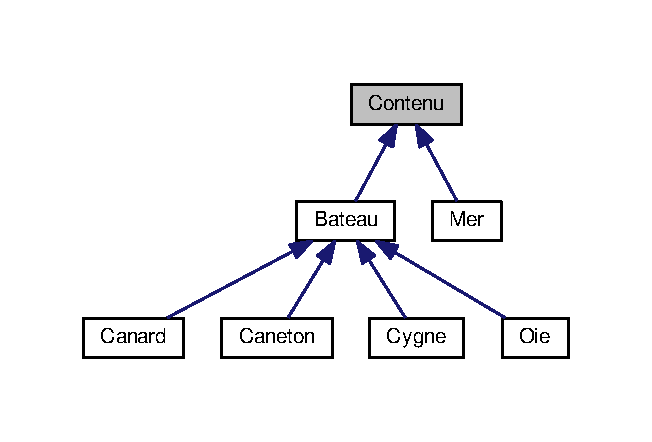
\includegraphics[width=313pt]{classContenu__inherit__graph}
\end{center}
\end{figure}
\subsection*{Public Member Functions}
\begin{DoxyCompactItemize}
\item 
\hyperlink{classContenu_ac20817eae49d031383e9a3be58c2bf15}{Contenu} ()
\begin{DoxyCompactList}\small\item\em Constructeur. \end{DoxyCompactList}\item 
virtual bool \hyperlink{classContenu_ae54145207bfdae5a24ce2c8c523c74a0}{action} (\hyperlink{classCase}{Case} $\ast$c)=0
\begin{DoxyCompactList}\small\item\em Action émise lorsqu'on a cliqué sur une \hyperlink{classCase}{Case}. \end{DoxyCompactList}\item 
virtual void \hyperlink{classContenu_a801fc9cb327750d2889ab3e7b185c029}{set\+X} (int x)=0
\begin{DoxyCompactList}\small\item\em Modifie la coordonnée X du \hyperlink{classContenu}{Contenu}. \end{DoxyCompactList}\item 
virtual void \hyperlink{classContenu_afc6fc6f669313fe77ca57559475d1750}{set\+Y} (int y)=0
\begin{DoxyCompactList}\small\item\em Modifie la coordonnée Y du \hyperlink{classContenu}{Contenu}. \end{DoxyCompactList}\item 
virtual void \hyperlink{classContenu_ad06f3204769fdc758a5859fbb7cac637}{set\+Horizontal} (bool a)=0
\begin{DoxyCompactList}\small\item\em Modifie l'orientation du \hyperlink{classBateau}{Bateau}. \end{DoxyCompactList}\item 
virtual int \hyperlink{classContenu_afce83627ee635c60edb0edced8191af4}{get\+X} ()=0
\begin{DoxyCompactList}\small\item\em Récupère la ligne où se trouve le \hyperlink{classContenu}{Contenu}. \end{DoxyCompactList}\item 
virtual int \hyperlink{classContenu_a1087d1609ec4842bb3d2a5dd960359b6}{get\+Y} ()=0
\begin{DoxyCompactList}\small\item\em Récupère la colonne où se trouve le \hyperlink{classContenu}{Contenu}. \end{DoxyCompactList}\item 
virtual bool \hyperlink{classContenu_aa9b4dbb3de416310cd53422a0d14879b}{get\+Horizontal} ()=0
\begin{DoxyCompactList}\small\item\em Récupère l'orientation du \hyperlink{classContenu}{Contenu}. \end{DoxyCompactList}\item 
virtual int \hyperlink{classContenu_abba99a1726eb744067cca7deb571444b}{get\+Taille} ()=0
\begin{DoxyCompactList}\small\item\em Connaitre la taille du \hyperlink{classContenu}{Contenu}. \end{DoxyCompactList}\item 
virtual bool \hyperlink{classContenu_a426053a6e632f1963c1c59c1515c99fb}{is\+Empty} ()=0
\begin{DoxyCompactList}\small\item\em Savoir si le contenu est vide. \end{DoxyCompactList}\item 
virtual bool \hyperlink{classContenu_af917356550ccc6025373c652b6e8b938}{touche} ()=0
\begin{DoxyCompactList}\small\item\em Savoir si le \hyperlink{classContenu}{Contenu} est touché \end{DoxyCompactList}\item 
virtual bool \hyperlink{classContenu_ad8ba918a8d5a08e4f8c0c742778500d6}{est\+Coule} ()=0
\begin{DoxyCompactList}\small\item\em Savoir si le \hyperlink{classContenu}{Contenu} est coulé \end{DoxyCompactList}\item 
\hypertarget{classContenu_a77f59e494b5c0f00ceb2da8d0067d4b8}{virtual \hyperlink{classContenu_a77f59e494b5c0f00ceb2da8d0067d4b8}{$\sim$\+Contenu} ()}\label{classContenu_a77f59e494b5c0f00ceb2da8d0067d4b8}

\begin{DoxyCompactList}\small\item\em Destructeur Destructeur de la classe \hyperlink{classContenu}{Contenu}. \end{DoxyCompactList}\end{DoxyCompactItemize}
\subsection*{Protected Attributes}
\begin{DoxyCompactItemize}
\item 
int \hyperlink{classContenu_a181b4b730433d5f2775d0c19cadd4132}{x\+\_\+}
\item 
int \hyperlink{classContenu_a571f1aa960aaaa1971bfefe70326457d}{y\+\_\+}
\item 
bool \hyperlink{classContenu_a7512c8fe29c284d31c24bfe03a6b2684}{horizontal\+\_\+}
\item 
int \hyperlink{classContenu_a354281d1fa2b2e8e39ee84c56115a7f5}{taille\+\_\+}
\end{DoxyCompactItemize}


\subsection{Detailed Description}
classe representant un \hyperlink{classContenu}{Contenu} 

La classe gère l'ensemble des comportements sur un contenu de cases 

\subsection{Constructor \& Destructor Documentation}
\hypertarget{classContenu_ac20817eae49d031383e9a3be58c2bf15}{\index{Contenu@{Contenu}!Contenu@{Contenu}}
\index{Contenu@{Contenu}!Contenu@{Contenu}}
\subsubsection[{Contenu}]{\setlength{\rightskip}{0pt plus 5cm}Contenu\+::\+Contenu (
\begin{DoxyParamCaption}
{}
\end{DoxyParamCaption}
)}}\label{classContenu_ac20817eae49d031383e9a3be58c2bf15}


Constructeur. 

Constructeur de la classe \hyperlink{classContenu}{Contenu} 

\subsection{Member Function Documentation}
\hypertarget{classContenu_ae54145207bfdae5a24ce2c8c523c74a0}{\index{Contenu@{Contenu}!action@{action}}
\index{action@{action}!Contenu@{Contenu}}
\subsubsection[{action}]{\setlength{\rightskip}{0pt plus 5cm}virtual bool Contenu\+::action (
\begin{DoxyParamCaption}
\item[{{\bf Case} $\ast$}]{c}
\end{DoxyParamCaption}
)\hspace{0.3cm}{\ttfamily [pure virtual]}}}\label{classContenu_ae54145207bfdae5a24ce2c8c523c74a0}


Action émise lorsqu'on a cliqué sur une \hyperlink{classCase}{Case}. 

Méthode permettant de savoir si le contenu de la case est un \hyperlink{classBateau}{Bateau} ou de la \hyperlink{classMer}{Mer}


\begin{DoxyParams}{Parameters}
{\em c} & \+: la case sur laquelle on a cliqué\\
\hline
\end{DoxyParams}
\begin{DoxyReturn}{Returns}
true si le contenu de la case est un \hyperlink{classBateau}{Bateau} sinon false 
\end{DoxyReturn}


Implemented in \hyperlink{classBateau_a3e54040953962f545b5fabadbcc330e8}{Bateau}, and \hyperlink{classMer_aa30fffa94a8e0d5be6ae503aa8392973}{Mer}.

\hypertarget{classContenu_ad8ba918a8d5a08e4f8c0c742778500d6}{\index{Contenu@{Contenu}!est\+Coule@{est\+Coule}}
\index{est\+Coule@{est\+Coule}!Contenu@{Contenu}}
\subsubsection[{est\+Coule}]{\setlength{\rightskip}{0pt plus 5cm}virtual bool Contenu\+::est\+Coule (
\begin{DoxyParamCaption}
{}
\end{DoxyParamCaption}
)\hspace{0.3cm}{\ttfamily [pure virtual]}}}\label{classContenu_ad8ba918a8d5a08e4f8c0c742778500d6}


Savoir si le \hyperlink{classContenu}{Contenu} est coulé 

Méthode permettant de savoir si le \hyperlink{classContenu}{Contenu} n'a plus de vie

\begin{DoxyReturn}{Returns}
true si le \hyperlink{classContenu}{Contenu} n'a plus de vie, false sinon 
\end{DoxyReturn}


Implemented in \hyperlink{classBateau_a6e4d8fc7cf8b265592dd009ecac72be2}{Bateau}, and \hyperlink{classMer_aa1a5b5633f2d7590e3074bf70a867ee0}{Mer}.

\hypertarget{classContenu_aa9b4dbb3de416310cd53422a0d14879b}{\index{Contenu@{Contenu}!get\+Horizontal@{get\+Horizontal}}
\index{get\+Horizontal@{get\+Horizontal}!Contenu@{Contenu}}
\subsubsection[{get\+Horizontal}]{\setlength{\rightskip}{0pt plus 5cm}virtual bool Contenu\+::get\+Horizontal (
\begin{DoxyParamCaption}
{}
\end{DoxyParamCaption}
)\hspace{0.3cm}{\ttfamily [pure virtual]}}}\label{classContenu_aa9b4dbb3de416310cd53422a0d14879b}


Récupère l'orientation du \hyperlink{classContenu}{Contenu}. 

Méthode permettant de savoir si le \hyperlink{classContenu}{Contenu} est horizontal ou vertical

\begin{DoxyReturn}{Returns}
true si le \hyperlink{classContenu}{Contenu} est horizontal, false sinon 
\end{DoxyReturn}


Implemented in \hyperlink{classBateau_a8578b6073e4f546d4c255e23fbb3c1dc}{Bateau}, and \hyperlink{classMer_aa2cfaf3bb10d817c535b843724759bc7}{Mer}.

\hypertarget{classContenu_abba99a1726eb744067cca7deb571444b}{\index{Contenu@{Contenu}!get\+Taille@{get\+Taille}}
\index{get\+Taille@{get\+Taille}!Contenu@{Contenu}}
\subsubsection[{get\+Taille}]{\setlength{\rightskip}{0pt plus 5cm}virtual int Contenu\+::get\+Taille (
\begin{DoxyParamCaption}
{}
\end{DoxyParamCaption}
)\hspace{0.3cm}{\ttfamily [pure virtual]}}}\label{classContenu_abba99a1726eb744067cca7deb571444b}


Connaitre la taille du \hyperlink{classContenu}{Contenu}. 

Méthode permettant de connaitre la taille du \hyperlink{classContenu}{Contenu}

\begin{DoxyReturn}{Returns}
la taille du \hyperlink{classContenu}{Contenu} 
\end{DoxyReturn}


Implemented in \hyperlink{classBateau_a08be20b8c871149d717a30b00c1068b9}{Bateau}, \hyperlink{classMer_ad3662e679f566da98a77b585d1699a7e}{Mer}, \hyperlink{classCanard_a5c99dcdcd79601f9cc075072c6fa8e47}{Canard}, \hyperlink{classCaneton_a173cbd22638bbf2806a47c329284ceee}{Caneton}, \hyperlink{classCygne_a48ec6800d6f11358be648cbe9a5fceb0}{Cygne}, and \hyperlink{classOie_aa07fdf5abd6eec1a4578a90edb029ad1}{Oie}.

\hypertarget{classContenu_afce83627ee635c60edb0edced8191af4}{\index{Contenu@{Contenu}!get\+X@{get\+X}}
\index{get\+X@{get\+X}!Contenu@{Contenu}}
\subsubsection[{get\+X}]{\setlength{\rightskip}{0pt plus 5cm}virtual int Contenu\+::get\+X (
\begin{DoxyParamCaption}
{}
\end{DoxyParamCaption}
)\hspace{0.3cm}{\ttfamily [pure virtual]}}}\label{classContenu_afce83627ee635c60edb0edced8191af4}


Récupère la ligne où se trouve le \hyperlink{classContenu}{Contenu}. 

Méthode permettant de récupérer la ligne sur laquelle se situe le \hyperlink{classContenu}{Contenu} de la \hyperlink{classCase}{Case}

\begin{DoxyReturn}{Returns}
le numéro de ligne sur laquelle se trouve le \hyperlink{classContenu}{Contenu} 
\end{DoxyReturn}


Implemented in \hyperlink{classBateau_ab7bd97ef05abea97c5322a16760b7d51}{Bateau}, and \hyperlink{classMer_a668a9c3acfa903bb7c8e1d607e1229a4}{Mer}.

\hypertarget{classContenu_a1087d1609ec4842bb3d2a5dd960359b6}{\index{Contenu@{Contenu}!get\+Y@{get\+Y}}
\index{get\+Y@{get\+Y}!Contenu@{Contenu}}
\subsubsection[{get\+Y}]{\setlength{\rightskip}{0pt plus 5cm}virtual int Contenu\+::get\+Y (
\begin{DoxyParamCaption}
{}
\end{DoxyParamCaption}
)\hspace{0.3cm}{\ttfamily [pure virtual]}}}\label{classContenu_a1087d1609ec4842bb3d2a5dd960359b6}


Récupère la colonne où se trouve le \hyperlink{classContenu}{Contenu}. 

Méthode permettant de récupérer la colonne sur laquelle se situe le \hyperlink{classContenu}{Contenu} de la \hyperlink{classCase}{Case}

\begin{DoxyReturn}{Returns}
le numéro de colonne sur laquelle se trouve le \hyperlink{classContenu}{Contenu} 
\end{DoxyReturn}


Implemented in \hyperlink{classBateau_a178bb83641412590fcc39d8974d6562a}{Bateau}, and \hyperlink{classMer_a41f5d00f824057af9c9b57d666bf6fcc}{Mer}.

\hypertarget{classContenu_a426053a6e632f1963c1c59c1515c99fb}{\index{Contenu@{Contenu}!is\+Empty@{is\+Empty}}
\index{is\+Empty@{is\+Empty}!Contenu@{Contenu}}
\subsubsection[{is\+Empty}]{\setlength{\rightskip}{0pt plus 5cm}virtual bool Contenu\+::is\+Empty (
\begin{DoxyParamCaption}
{}
\end{DoxyParamCaption}
)\hspace{0.3cm}{\ttfamily [pure virtual]}}}\label{classContenu_a426053a6e632f1963c1c59c1515c99fb}


Savoir si le contenu est vide. 

Méthode permettant de savoir si le contenu est vide ( de la \hyperlink{classMer}{Mer} )

\begin{DoxyReturn}{Returns}
true s'il s'agit d'un \hyperlink{classBateau}{Bateau}, false si c'est de la \hyperlink{classMer}{Mer} 
\end{DoxyReturn}


Implemented in \hyperlink{classBateau_a8a8984f7b1010fbdd4cd15c7768da2ca}{Bateau}, and \hyperlink{classMer_ac76c2299715ae08f07e8a9fc0821b032}{Mer}.

\hypertarget{classContenu_ad06f3204769fdc758a5859fbb7cac637}{\index{Contenu@{Contenu}!set\+Horizontal@{set\+Horizontal}}
\index{set\+Horizontal@{set\+Horizontal}!Contenu@{Contenu}}
\subsubsection[{set\+Horizontal}]{\setlength{\rightskip}{0pt plus 5cm}virtual void Contenu\+::set\+Horizontal (
\begin{DoxyParamCaption}
\item[{bool}]{a}
\end{DoxyParamCaption}
)\hspace{0.3cm}{\ttfamily [pure virtual]}}}\label{classContenu_ad06f3204769fdc758a5859fbb7cac637}


Modifie l'orientation du \hyperlink{classBateau}{Bateau}. 

Méthode permettant de modifier l'orientation du \hyperlink{classContenu}{Contenu}


\begin{DoxyParams}{Parameters}
{\em a} & \+: booléen à true \+: horizontal, sinon vertical \\
\hline
\end{DoxyParams}


Implemented in \hyperlink{classBateau_a1dae1dbd3d3e0334a4dc5b43ef579c25}{Bateau}, and \hyperlink{classMer_a3244c63c7b077ef84e593d9b5e5f4472}{Mer}.

\hypertarget{classContenu_a801fc9cb327750d2889ab3e7b185c029}{\index{Contenu@{Contenu}!set\+X@{set\+X}}
\index{set\+X@{set\+X}!Contenu@{Contenu}}
\subsubsection[{set\+X}]{\setlength{\rightskip}{0pt plus 5cm}virtual void Contenu\+::set\+X (
\begin{DoxyParamCaption}
\item[{int}]{x}
\end{DoxyParamCaption}
)\hspace{0.3cm}{\ttfamily [pure virtual]}}}\label{classContenu_a801fc9cb327750d2889ab3e7b185c029}


Modifie la coordonnée X du \hyperlink{classContenu}{Contenu}. 

Méthode permettant de modifier la coordonnée en X, c'est à dire sur quelle ligne placer le \hyperlink{classContenu}{Contenu}


\begin{DoxyParams}{Parameters}
{\em x} & \+: numéro de la ligne \\
\hline
\end{DoxyParams}


Implemented in \hyperlink{classBateau_a12cc2226f5533d98b5b1f71fc042f1a6}{Bateau}, and \hyperlink{classMer_ab20617d436898cc631fc1842e897de0c}{Mer}.

\hypertarget{classContenu_afc6fc6f669313fe77ca57559475d1750}{\index{Contenu@{Contenu}!set\+Y@{set\+Y}}
\index{set\+Y@{set\+Y}!Contenu@{Contenu}}
\subsubsection[{set\+Y}]{\setlength{\rightskip}{0pt plus 5cm}virtual void Contenu\+::set\+Y (
\begin{DoxyParamCaption}
\item[{int}]{y}
\end{DoxyParamCaption}
)\hspace{0.3cm}{\ttfamily [pure virtual]}}}\label{classContenu_afc6fc6f669313fe77ca57559475d1750}


Modifie la coordonnée Y du \hyperlink{classContenu}{Contenu}. 

Méthode permettant de modifier la coordonnée en Y, c'est à dire sur quelle colonne placer le \hyperlink{classContenu}{Contenu}


\begin{DoxyParams}{Parameters}
{\em x} & \+: numéro de la colonne \\
\hline
\end{DoxyParams}


Implemented in \hyperlink{classBateau_ad84a941f5968a3690b80b12ca56547c4}{Bateau}, and \hyperlink{classMer_a13ac62cb31e498d5bcf786d5a0d196ed}{Mer}.

\hypertarget{classContenu_af917356550ccc6025373c652b6e8b938}{\index{Contenu@{Contenu}!touche@{touche}}
\index{touche@{touche}!Contenu@{Contenu}}
\subsubsection[{touche}]{\setlength{\rightskip}{0pt plus 5cm}virtual bool Contenu\+::touche (
\begin{DoxyParamCaption}
{}
\end{DoxyParamCaption}
)\hspace{0.3cm}{\ttfamily [pure virtual]}}}\label{classContenu_af917356550ccc6025373c652b6e8b938}


Savoir si le \hyperlink{classContenu}{Contenu} est touché 

Méthode permettant de savoir si le \hyperlink{classContenu}{Contenu} est touché

\begin{DoxyReturn}{Returns}
true si le \hyperlink{classContenu}{Contenu} est un \hyperlink{classBateau}{Bateau}, false si c'est de la \hyperlink{classMer}{Mer} 
\end{DoxyReturn}


Implemented in \hyperlink{classBateau_a8fff831d5081544b0abbf5b6816ebe35}{Bateau}, and \hyperlink{classMer_a2ec6ecba14a8f737335720f3dffe9877}{Mer}.



\subsection{Member Data Documentation}
\hypertarget{classContenu_a7512c8fe29c284d31c24bfe03a6b2684}{\index{Contenu@{Contenu}!horizontal\+\_\+@{horizontal\+\_\+}}
\index{horizontal\+\_\+@{horizontal\+\_\+}!Contenu@{Contenu}}
\subsubsection[{horizontal\+\_\+}]{\setlength{\rightskip}{0pt plus 5cm}bool Contenu\+::horizontal\+\_\+\hspace{0.3cm}{\ttfamily [protected]}}}\label{classContenu_a7512c8fe29c284d31c24bfe03a6b2684}
l'orientation du contenu \hypertarget{classContenu_a354281d1fa2b2e8e39ee84c56115a7f5}{\index{Contenu@{Contenu}!taille\+\_\+@{taille\+\_\+}}
\index{taille\+\_\+@{taille\+\_\+}!Contenu@{Contenu}}
\subsubsection[{taille\+\_\+}]{\setlength{\rightskip}{0pt plus 5cm}int Contenu\+::taille\+\_\+\hspace{0.3cm}{\ttfamily [protected]}}}\label{classContenu_a354281d1fa2b2e8e39ee84c56115a7f5}
la taille du contenu \hypertarget{classContenu_a181b4b730433d5f2775d0c19cadd4132}{\index{Contenu@{Contenu}!x\+\_\+@{x\+\_\+}}
\index{x\+\_\+@{x\+\_\+}!Contenu@{Contenu}}
\subsubsection[{x\+\_\+}]{\setlength{\rightskip}{0pt plus 5cm}int Contenu\+::x\+\_\+\hspace{0.3cm}{\ttfamily [protected]}}}\label{classContenu_a181b4b730433d5f2775d0c19cadd4132}
le numéro de ligne du \hyperlink{classContenu}{Contenu} \hypertarget{classContenu_a571f1aa960aaaa1971bfefe70326457d}{\index{Contenu@{Contenu}!y\+\_\+@{y\+\_\+}}
\index{y\+\_\+@{y\+\_\+}!Contenu@{Contenu}}
\subsubsection[{y\+\_\+}]{\setlength{\rightskip}{0pt plus 5cm}int Contenu\+::y\+\_\+\hspace{0.3cm}{\ttfamily [protected]}}}\label{classContenu_a571f1aa960aaaa1971bfefe70326457d}
le numéro de colonne du \hyperlink{classContenu}{Contenu} 

The documentation for this interface was generated from the following files\+:\begin{DoxyCompactItemize}
\item 
contenu.\+h\item 
contenu.\+cpp\end{DoxyCompactItemize}

\hypertarget{classCore}{\section{Core Class Reference}
\label{classCore}\index{Core@{Core}}
}


classe representant le coeur de l'application  




{\ttfamily \#include $<$core.\+h$>$}

\subsection*{Public Member Functions}
\begin{DoxyCompactItemize}
\item 
\hyperlink{classCore_a14e63188e0aa7c4a6f72d5501384d1f9}{Core} ()
\begin{DoxyCompactList}\small\item\em Constructeur. \end{DoxyCompactList}\item 
void \hyperlink{classCore_aefcf76351ec813fb99f39fbcce42afac}{change\+Mode} (\hyperlink{classCompMode}{Comp\+Mode} $\ast$mode)
\begin{DoxyCompactList}\small\item\em Changer le mode de jeu. \end{DoxyCompactList}\item 
void \hyperlink{classCore_aeb0646c87941a9120d85bbe3f5fb8700}{afficher} ()
\begin{DoxyCompactList}\small\item\em Permet d'afficher l'affichage actif. \end{DoxyCompactList}\item 
std\+::shared\+\_\+ptr$<$ \hyperlink{classTeam}{Team} $>$ \hyperlink{classCore_ab8696ef45b3d2d52ffbbe8a591dc99fb}{get\+Team1} ()
\begin{DoxyCompactList}\small\item\em Récupère le J1. \end{DoxyCompactList}\item 
std\+::shared\+\_\+ptr$<$ \hyperlink{classTeam}{Team} $>$ \hyperlink{classCore_ae2a1b22acb1cc7a021c279b22e5c1cc1}{get\+Team2} ()
\begin{DoxyCompactList}\small\item\em Récupère le J2. \end{DoxyCompactList}\item 
std\+::shared\+\_\+ptr$<$ \hyperlink{classCompMode}{Comp\+Mode} $>$ \hyperlink{classCore_ae18939eeb844be8ec6960af11ddc31db}{get\+Mode} ()
\begin{DoxyCompactList}\small\item\em Récupère le mode de jeu. \end{DoxyCompactList}\item 
void \hyperlink{classCore_aa9f91b5e846906e97f1ba479ae3c1cc1}{change\+Affichage\+To\+Jeu} ()
\begin{DoxyCompactList}\small\item\em Change l'affichage vers le celui de jeu. \end{DoxyCompactList}\item 
void \hyperlink{classCore_aa6e820eee8d7479036e082652474006e}{change\+Affichage\+To\+Menu} ()
\begin{DoxyCompactList}\small\item\em Change l'affichage vers le celui du menu. \end{DoxyCompactList}\item 
void \hyperlink{classCore_a3a83d27d66ff842b74f8399c483973b1}{change\+Affichage\+To\+Init\+J1} ()
\begin{DoxyCompactList}\small\item\em Change l'affichage vers le celui de l'initialisation pour le J1. \end{DoxyCompactList}\item 
void \hyperlink{classCore_a7dde7558331088ab7d57572477fc8f2b}{change\+Affichage\+To\+Init\+J2} ()
\begin{DoxyCompactList}\small\item\em Change l'affichage vers le celui de l'initialisation pour le J2. \end{DoxyCompactList}\item 
void \hyperlink{classCore_abc88e9e2f23f9df672ffc987ea29d329}{fin\+Init\+J1} ()
\begin{DoxyCompactList}\small\item\em Change l'affichage vers le celui de l'initialisation pour le J2. \end{DoxyCompactList}\item 
void \hyperlink{classCore_af10b83849055258108b9769617edb5e5}{fin\+Init\+J2} ()
\begin{DoxyCompactList}\small\item\em Change l'affichage vers le celui du jeu selon le mode. \end{DoxyCompactList}\item 
void \hyperlink{classCore_a0a45f16dc5613ac2239f8648befb59c4}{set\+Image\+Chgmt\+Tour} ()
\begin{DoxyCompactList}\small\item\em Tourne l'image pour l'\hyperlink{classAffichageJeu}{Affichage\+Jeu} pour le tour des joueurs. \end{DoxyCompactList}\item 
\hypertarget{classCore_a776f8c46504b14183883c6273f93eaed}{virtual \hyperlink{classCore_a776f8c46504b14183883c6273f93eaed}{$\sim$\+Core} ()}\label{classCore_a776f8c46504b14183883c6273f93eaed}

\begin{DoxyCompactList}\small\item\em Destructeur Destructeur de la classe \hyperlink{classCore}{Core}. \end{DoxyCompactList}\end{DoxyCompactItemize}
\subsection*{Protected Attributes}
\begin{DoxyCompactItemize}
\item 
std\+::shared\+\_\+ptr$<$ \hyperlink{classCompMode}{Comp\+Mode} $>$ \hyperlink{classCore_ab7d2af28daa772c12d0a2cea6e65f887}{mode\+\_\+}
\item 
std\+::shared\+\_\+ptr$<$ \hyperlink{classTeam}{Team} $>$ \hyperlink{classCore_a299a0b1ed101953462d17c6e0528b006}{team1\+\_\+}
\item 
std\+::shared\+\_\+ptr$<$ \hyperlink{classTeam}{Team} $>$ \hyperlink{classCore_a4e9f0791fb0449a8c4b0ccce607a11da}{team2\+\_\+}
\item 
std\+::shared\+\_\+ptr$<$ \hyperlink{classIAffichage}{I\+Affichage} $>$ \hyperlink{classCore_ace6812af8ec428d12258d5c895a1fb2d}{affichage\+Actif\+\_\+}
\item 
std\+::shared\+\_\+ptr$<$ \hyperlink{classAffichageJeu}{Affichage\+Jeu} $>$ \hyperlink{classCore_a2558f752fb1c060782d4f75d9d09b864}{aff\+Jeu\+\_\+}
\item 
std\+::shared\+\_\+ptr$<$ \hyperlink{classIAffichage}{I\+Affichage} $>$ \hyperlink{classCore_a2d9a9ba8be0844338f67e8feab39ba9e}{aff\+Men\+\_\+}
\item 
std\+::shared\+\_\+ptr$<$ \hyperlink{classIAffichage}{I\+Affichage} $>$ \hyperlink{classCore_af1b29bd6eb49663e39efff0a91d9c9df}{aff\+Ini\+J1\+\_\+}
\item 
std\+::shared\+\_\+ptr$<$ \hyperlink{classIAffichage}{I\+Affichage} $>$ \hyperlink{classCore_a4d85e8590561c684900e1a2fd18184e2}{aff\+Ini\+J2\+\_\+}
\end{DoxyCompactItemize}


\subsection{Detailed Description}
classe representant le coeur de l'application 

La classe gère l'ensemble des actions entre les classes 

\subsection{Constructor \& Destructor Documentation}
\hypertarget{classCore_a14e63188e0aa7c4a6f72d5501384d1f9}{\index{Core@{Core}!Core@{Core}}
\index{Core@{Core}!Core@{Core}}
\subsubsection[{Core}]{\setlength{\rightskip}{0pt plus 5cm}Core\+::\+Core (
\begin{DoxyParamCaption}
{}
\end{DoxyParamCaption}
)}}\label{classCore_a14e63188e0aa7c4a6f72d5501384d1f9}


Constructeur. 

Constructeur de la classe \hyperlink{classCore}{Core} 

\subsection{Member Function Documentation}
\hypertarget{classCore_aeb0646c87941a9120d85bbe3f5fb8700}{\index{Core@{Core}!afficher@{afficher}}
\index{afficher@{afficher}!Core@{Core}}
\subsubsection[{afficher}]{\setlength{\rightskip}{0pt plus 5cm}void Core\+::afficher (
\begin{DoxyParamCaption}
{}
\end{DoxyParamCaption}
)}}\label{classCore_aeb0646c87941a9120d85bbe3f5fb8700}


Permet d'afficher l'affichage actif. 

Méthode permettant de déléguer l'affichage à l'affichage actif \hypertarget{classCore_a3a83d27d66ff842b74f8399c483973b1}{\index{Core@{Core}!change\+Affichage\+To\+Init\+J1@{change\+Affichage\+To\+Init\+J1}}
\index{change\+Affichage\+To\+Init\+J1@{change\+Affichage\+To\+Init\+J1}!Core@{Core}}
\subsubsection[{change\+Affichage\+To\+Init\+J1}]{\setlength{\rightskip}{0pt plus 5cm}void Core\+::change\+Affichage\+To\+Init\+J1 (
\begin{DoxyParamCaption}
{}
\end{DoxyParamCaption}
)}}\label{classCore_a3a83d27d66ff842b74f8399c483973b1}


Change l'affichage vers le celui de l'initialisation pour le J1. 

Méthode pour cacher l'affichage courant avec celui de l'initialisation du J1 \hypertarget{classCore_a7dde7558331088ab7d57572477fc8f2b}{\index{Core@{Core}!change\+Affichage\+To\+Init\+J2@{change\+Affichage\+To\+Init\+J2}}
\index{change\+Affichage\+To\+Init\+J2@{change\+Affichage\+To\+Init\+J2}!Core@{Core}}
\subsubsection[{change\+Affichage\+To\+Init\+J2}]{\setlength{\rightskip}{0pt plus 5cm}void Core\+::change\+Affichage\+To\+Init\+J2 (
\begin{DoxyParamCaption}
{}
\end{DoxyParamCaption}
)}}\label{classCore_a7dde7558331088ab7d57572477fc8f2b}


Change l'affichage vers le celui de l'initialisation pour le J2. 

Méthode pour cacher l'affichage courant avec celui de l'initialisation du J2 \hypertarget{classCore_aa9f91b5e846906e97f1ba479ae3c1cc1}{\index{Core@{Core}!change\+Affichage\+To\+Jeu@{change\+Affichage\+To\+Jeu}}
\index{change\+Affichage\+To\+Jeu@{change\+Affichage\+To\+Jeu}!Core@{Core}}
\subsubsection[{change\+Affichage\+To\+Jeu}]{\setlength{\rightskip}{0pt plus 5cm}void Core\+::change\+Affichage\+To\+Jeu (
\begin{DoxyParamCaption}
{}
\end{DoxyParamCaption}
)}}\label{classCore_aa9f91b5e846906e97f1ba479ae3c1cc1}


Change l'affichage vers le celui de jeu. 

Méthode pour cacher l'affichage courant avec celui du jeu \hypertarget{classCore_aa6e820eee8d7479036e082652474006e}{\index{Core@{Core}!change\+Affichage\+To\+Menu@{change\+Affichage\+To\+Menu}}
\index{change\+Affichage\+To\+Menu@{change\+Affichage\+To\+Menu}!Core@{Core}}
\subsubsection[{change\+Affichage\+To\+Menu}]{\setlength{\rightskip}{0pt plus 5cm}void Core\+::change\+Affichage\+To\+Menu (
\begin{DoxyParamCaption}
{}
\end{DoxyParamCaption}
)}}\label{classCore_aa6e820eee8d7479036e082652474006e}


Change l'affichage vers le celui du menu. 

Méthode pour cacher l'affichage courant avec celui du menu \hypertarget{classCore_aefcf76351ec813fb99f39fbcce42afac}{\index{Core@{Core}!change\+Mode@{change\+Mode}}
\index{change\+Mode@{change\+Mode}!Core@{Core}}
\subsubsection[{change\+Mode}]{\setlength{\rightskip}{0pt plus 5cm}void Core\+::change\+Mode (
\begin{DoxyParamCaption}
\item[{{\bf Comp\+Mode} $\ast$}]{mode}
\end{DoxyParamCaption}
)}}\label{classCore_aefcf76351ec813fb99f39fbcce42afac}


Changer le mode de jeu. 

Méthode permettant de passer du mode 1\+V1 vers 1\+V\+I\+A et inversement


\begin{DoxyParams}{Parameters}
{\em mode} & \+: le nouveau mode de jeu \\
\hline
\end{DoxyParams}
\hypertarget{classCore_abc88e9e2f23f9df672ffc987ea29d329}{\index{Core@{Core}!fin\+Init\+J1@{fin\+Init\+J1}}
\index{fin\+Init\+J1@{fin\+Init\+J1}!Core@{Core}}
\subsubsection[{fin\+Init\+J1}]{\setlength{\rightskip}{0pt plus 5cm}void Core\+::fin\+Init\+J1 (
\begin{DoxyParamCaption}
{}
\end{DoxyParamCaption}
)}}\label{classCore_abc88e9e2f23f9df672ffc987ea29d329}


Change l'affichage vers le celui de l'initialisation pour le J2. 

Méthode pour cacher l'affichage courant avec celui de l'initialisation du J2 \hypertarget{classCore_af10b83849055258108b9769617edb5e5}{\index{Core@{Core}!fin\+Init\+J2@{fin\+Init\+J2}}
\index{fin\+Init\+J2@{fin\+Init\+J2}!Core@{Core}}
\subsubsection[{fin\+Init\+J2}]{\setlength{\rightskip}{0pt plus 5cm}void Core\+::fin\+Init\+J2 (
\begin{DoxyParamCaption}
{}
\end{DoxyParamCaption}
)}}\label{classCore_af10b83849055258108b9769617edb5e5}


Change l'affichage vers le celui du jeu selon le mode. 

Méthode pour cacher l'affichage courant avec celui du jeu selon le mode avec 1\+V1 \+: on passe au jeu avec 1\+V\+I\+A \+: on passe au jeu après avoir initialiser automatiquement le J2 \hypertarget{classCore_ae18939eeb844be8ec6960af11ddc31db}{\index{Core@{Core}!get\+Mode@{get\+Mode}}
\index{get\+Mode@{get\+Mode}!Core@{Core}}
\subsubsection[{get\+Mode}]{\setlength{\rightskip}{0pt plus 5cm}shared\+\_\+ptr$<$ {\bf Comp\+Mode} $>$ Core\+::get\+Mode (
\begin{DoxyParamCaption}
{}
\end{DoxyParamCaption}
)}}\label{classCore_ae18939eeb844be8ec6960af11ddc31db}


Récupère le mode de jeu. 

Méthode permettant de récupérer le mode de jeu actif

\begin{DoxyReturn}{Returns}
le mode de jeu actif 
\end{DoxyReturn}
\hypertarget{classCore_ab8696ef45b3d2d52ffbbe8a591dc99fb}{\index{Core@{Core}!get\+Team1@{get\+Team1}}
\index{get\+Team1@{get\+Team1}!Core@{Core}}
\subsubsection[{get\+Team1}]{\setlength{\rightskip}{0pt plus 5cm}shared\+\_\+ptr$<$ {\bf Team} $>$ Core\+::get\+Team1 (
\begin{DoxyParamCaption}
{}
\end{DoxyParamCaption}
)}}\label{classCore_ab8696ef45b3d2d52ffbbe8a591dc99fb}


Récupère le J1. 

Méthode permettant de récupérer le J1

\begin{DoxyReturn}{Returns}
le J1 
\end{DoxyReturn}
\hypertarget{classCore_ae2a1b22acb1cc7a021c279b22e5c1cc1}{\index{Core@{Core}!get\+Team2@{get\+Team2}}
\index{get\+Team2@{get\+Team2}!Core@{Core}}
\subsubsection[{get\+Team2}]{\setlength{\rightskip}{0pt plus 5cm}shared\+\_\+ptr$<$ {\bf Team} $>$ Core\+::get\+Team2 (
\begin{DoxyParamCaption}
{}
\end{DoxyParamCaption}
)}}\label{classCore_ae2a1b22acb1cc7a021c279b22e5c1cc1}


Récupère le J2. 

Méthode permettant de récupérer le J2

\begin{DoxyReturn}{Returns}
le J2 
\end{DoxyReturn}
\hypertarget{classCore_a0a45f16dc5613ac2239f8648befb59c4}{\index{Core@{Core}!set\+Image\+Chgmt\+Tour@{set\+Image\+Chgmt\+Tour}}
\index{set\+Image\+Chgmt\+Tour@{set\+Image\+Chgmt\+Tour}!Core@{Core}}
\subsubsection[{set\+Image\+Chgmt\+Tour}]{\setlength{\rightskip}{0pt plus 5cm}void Core\+::set\+Image\+Chgmt\+Tour (
\begin{DoxyParamCaption}
{}
\end{DoxyParamCaption}
)}}\label{classCore_a0a45f16dc5613ac2239f8648befb59c4}


Tourne l'image pour l'\hyperlink{classAffichageJeu}{Affichage\+Jeu} pour le tour des joueurs. 

Méthode qui est déléguée à l'\hyperlink{classAffichageJeu}{Affichage\+Jeu} 

\subsection{Member Data Documentation}
\hypertarget{classCore_ace6812af8ec428d12258d5c895a1fb2d}{\index{Core@{Core}!affichage\+Actif\+\_\+@{affichage\+Actif\+\_\+}}
\index{affichage\+Actif\+\_\+@{affichage\+Actif\+\_\+}!Core@{Core}}
\subsubsection[{affichage\+Actif\+\_\+}]{\setlength{\rightskip}{0pt plus 5cm}std\+::shared\+\_\+ptr$<${\bf I\+Affichage}$>$ Core\+::affichage\+Actif\+\_\+\hspace{0.3cm}{\ttfamily [protected]}}}\label{classCore_ace6812af8ec428d12258d5c895a1fb2d}
l'affichage actif qui prend pour valeur les différents affichages quand c'est nécessaire \hypertarget{classCore_af1b29bd6eb49663e39efff0a91d9c9df}{\index{Core@{Core}!aff\+Ini\+J1\+\_\+@{aff\+Ini\+J1\+\_\+}}
\index{aff\+Ini\+J1\+\_\+@{aff\+Ini\+J1\+\_\+}!Core@{Core}}
\subsubsection[{aff\+Ini\+J1\+\_\+}]{\setlength{\rightskip}{0pt plus 5cm}std\+::shared\+\_\+ptr$<${\bf I\+Affichage}$>$ Core\+::aff\+Ini\+J1\+\_\+\hspace{0.3cm}{\ttfamily [protected]}}}\label{classCore_af1b29bd6eb49663e39efff0a91d9c9df}
pour l'affichage de l'initialisation du J1 \hypertarget{classCore_a4d85e8590561c684900e1a2fd18184e2}{\index{Core@{Core}!aff\+Ini\+J2\+\_\+@{aff\+Ini\+J2\+\_\+}}
\index{aff\+Ini\+J2\+\_\+@{aff\+Ini\+J2\+\_\+}!Core@{Core}}
\subsubsection[{aff\+Ini\+J2\+\_\+}]{\setlength{\rightskip}{0pt plus 5cm}std\+::shared\+\_\+ptr$<${\bf I\+Affichage}$>$ Core\+::aff\+Ini\+J2\+\_\+\hspace{0.3cm}{\ttfamily [protected]}}}\label{classCore_a4d85e8590561c684900e1a2fd18184e2}
pour l'affichage de l'initialisation du J2 \hypertarget{classCore_a2558f752fb1c060782d4f75d9d09b864}{\index{Core@{Core}!aff\+Jeu\+\_\+@{aff\+Jeu\+\_\+}}
\index{aff\+Jeu\+\_\+@{aff\+Jeu\+\_\+}!Core@{Core}}
\subsubsection[{aff\+Jeu\+\_\+}]{\setlength{\rightskip}{0pt plus 5cm}std\+::shared\+\_\+ptr$<${\bf Affichage\+Jeu}$>$ Core\+::aff\+Jeu\+\_\+\hspace{0.3cm}{\ttfamily [protected]}}}\label{classCore_a2558f752fb1c060782d4f75d9d09b864}
pour l'affichage du jeu \hypertarget{classCore_a2d9a9ba8be0844338f67e8feab39ba9e}{\index{Core@{Core}!aff\+Men\+\_\+@{aff\+Men\+\_\+}}
\index{aff\+Men\+\_\+@{aff\+Men\+\_\+}!Core@{Core}}
\subsubsection[{aff\+Men\+\_\+}]{\setlength{\rightskip}{0pt plus 5cm}std\+::shared\+\_\+ptr$<${\bf I\+Affichage}$>$ Core\+::aff\+Men\+\_\+\hspace{0.3cm}{\ttfamily [protected]}}}\label{classCore_a2d9a9ba8be0844338f67e8feab39ba9e}
pour l'affichage du menu \hypertarget{classCore_ab7d2af28daa772c12d0a2cea6e65f887}{\index{Core@{Core}!mode\+\_\+@{mode\+\_\+}}
\index{mode\+\_\+@{mode\+\_\+}!Core@{Core}}
\subsubsection[{mode\+\_\+}]{\setlength{\rightskip}{0pt plus 5cm}std\+::shared\+\_\+ptr$<${\bf Comp\+Mode}$>$ Core\+::mode\+\_\+\hspace{0.3cm}{\ttfamily [protected]}}}\label{classCore_ab7d2af28daa772c12d0a2cea6e65f887}
correspond au mode de jeu \hypertarget{classCore_a299a0b1ed101953462d17c6e0528b006}{\index{Core@{Core}!team1\+\_\+@{team1\+\_\+}}
\index{team1\+\_\+@{team1\+\_\+}!Core@{Core}}
\subsubsection[{team1\+\_\+}]{\setlength{\rightskip}{0pt plus 5cm}std\+::shared\+\_\+ptr$<${\bf Team}$>$ Core\+::team1\+\_\+\hspace{0.3cm}{\ttfamily [protected]}}}\label{classCore_a299a0b1ed101953462d17c6e0528b006}
le J1 \hypertarget{classCore_a4e9f0791fb0449a8c4b0ccce607a11da}{\index{Core@{Core}!team2\+\_\+@{team2\+\_\+}}
\index{team2\+\_\+@{team2\+\_\+}!Core@{Core}}
\subsubsection[{team2\+\_\+}]{\setlength{\rightskip}{0pt plus 5cm}std\+::shared\+\_\+ptr$<${\bf Team}$>$ Core\+::team2\+\_\+\hspace{0.3cm}{\ttfamily [protected]}}}\label{classCore_a4e9f0791fb0449a8c4b0ccce607a11da}
le J2 

The documentation for this class was generated from the following files\+:\begin{DoxyCompactItemize}
\item 
core.\+h\item 
core.\+cpp\end{DoxyCompactItemize}

\hypertarget{classCygne}{\section{Cygne Class Reference}
\label{classCygne}\index{Cygne@{Cygne}}
}


classe representant un \hyperlink{classCygne}{Cygne}  




{\ttfamily \#include $<$cygne.\+h$>$}



Inheritance diagram for Cygne\+:
\nopagebreak
\begin{figure}[H]
\begin{center}
\leavevmode
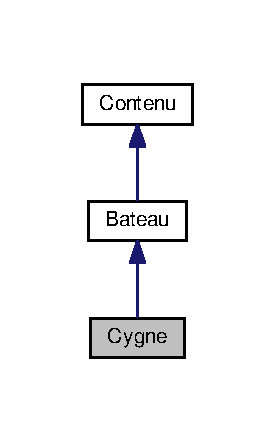
\includegraphics[width=132pt]{classCygne__inherit__graph}
\end{center}
\end{figure}


Collaboration diagram for Cygne\+:
\nopagebreak
\begin{figure}[H]
\begin{center}
\leavevmode
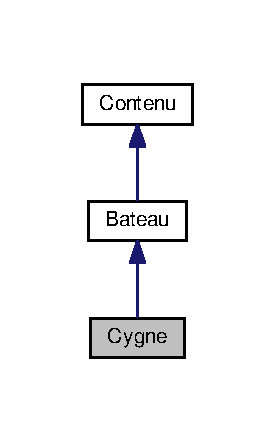
\includegraphics[width=132pt]{classCygne__coll__graph}
\end{center}
\end{figure}
\subsection*{Public Member Functions}
\begin{DoxyCompactItemize}
\item 
\hyperlink{classCygne_a5e27cc91418516c85dbffb6b032f9588}{Cygne} ()
\begin{DoxyCompactList}\small\item\em Constructeur. \end{DoxyCompactList}\item 
int \hyperlink{classCygne_a48ec6800d6f11358be648cbe9a5fceb0}{get\+Taille} ()
\begin{DoxyCompactList}\small\item\em Récupère la taille du \hyperlink{classBateau}{Bateau}. \end{DoxyCompactList}\end{DoxyCompactItemize}
\subsection*{Additional Inherited Members}


\subsection{Detailed Description}
classe representant un \hyperlink{classCygne}{Cygne} 

La classe modélise un \hyperlink{classBateau}{Bateau} de taille 4 

\subsection{Constructor \& Destructor Documentation}
\hypertarget{classCygne_a5e27cc91418516c85dbffb6b032f9588}{\index{Cygne@{Cygne}!Cygne@{Cygne}}
\index{Cygne@{Cygne}!Cygne@{Cygne}}
\subsubsection[{Cygne}]{\setlength{\rightskip}{0pt plus 5cm}Cygne\+::\+Cygne (
\begin{DoxyParamCaption}
{}
\end{DoxyParamCaption}
)}}\label{classCygne_a5e27cc91418516c85dbffb6b032f9588}


Constructeur. 

Constructeur de la classe \hyperlink{classCygne}{Cygne} 

\subsection{Member Function Documentation}
\hypertarget{classCygne_a48ec6800d6f11358be648cbe9a5fceb0}{\index{Cygne@{Cygne}!get\+Taille@{get\+Taille}}
\index{get\+Taille@{get\+Taille}!Cygne@{Cygne}}
\subsubsection[{get\+Taille}]{\setlength{\rightskip}{0pt plus 5cm}int Cygne\+::get\+Taille (
\begin{DoxyParamCaption}
{}
\end{DoxyParamCaption}
)\hspace{0.3cm}{\ttfamily [virtual]}}}\label{classCygne_a48ec6800d6f11358be648cbe9a5fceb0}


Récupère la taille du \hyperlink{classBateau}{Bateau}. 

Méthode permettant de récupérer la taille d'un \hyperlink{classCygne}{Cygne}

\begin{DoxyReturn}{Returns}
la taille d'un \hyperlink{classCygne}{Cygne} (4) 
\end{DoxyReturn}


Implements \hyperlink{classBateau_a08be20b8c871149d717a30b00c1068b9}{Bateau}.



The documentation for this class was generated from the following files\+:\begin{DoxyCompactItemize}
\item 
cygne.\+h\item 
cygne.\+cpp\end{DoxyCompactItemize}

\hypertarget{classFactoryCanard}{\section{Factory\+Canard Class Reference}
\label{classFactoryCanard}\index{Factory\+Canard@{Factory\+Canard}}
}


classe representant une usine à \hyperlink{classCanard}{Canard}  




{\ttfamily \#include $<$factorycanard.\+h$>$}



Inheritance diagram for Factory\+Canard\+:
\nopagebreak
\begin{figure}[H]
\begin{center}
\leavevmode
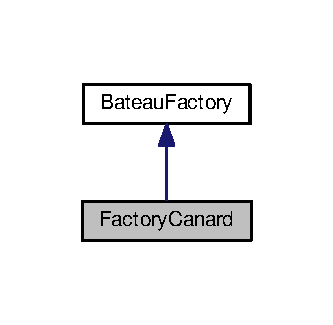
\includegraphics[width=160pt]{classFactoryCanard__inherit__graph}
\end{center}
\end{figure}


Collaboration diagram for Factory\+Canard\+:
\nopagebreak
\begin{figure}[H]
\begin{center}
\leavevmode
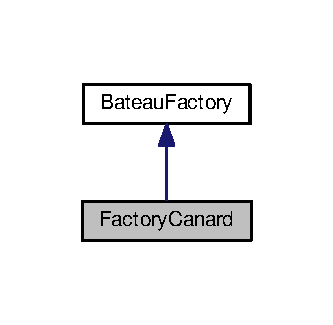
\includegraphics[width=160pt]{classFactoryCanard__coll__graph}
\end{center}
\end{figure}
\subsection*{Public Member Functions}
\begin{DoxyCompactItemize}
\item 
\hyperlink{classFactoryCanard_a3f272dfd46acb1b14900cc9f6c30a02a}{Factory\+Canard} ()
\begin{DoxyCompactList}\small\item\em Constructeur. \end{DoxyCompactList}\item 
std\+::shared\+\_\+ptr$<$ \hyperlink{classBateau}{Bateau} $>$ \hyperlink{classFactoryCanard_a3ef0d9a9c293006fb09fd03a911a1377}{creer\+Bateau} ()
\begin{DoxyCompactList}\small\item\em Récupère le \hyperlink{classCanard}{Canard} créé \end{DoxyCompactList}\end{DoxyCompactItemize}


\subsection{Detailed Description}
classe representant une usine à \hyperlink{classCanard}{Canard} 

La classe modélise une usine à \hyperlink{classBateau}{Bateau} de taille 2 

\subsection{Constructor \& Destructor Documentation}
\hypertarget{classFactoryCanard_a3f272dfd46acb1b14900cc9f6c30a02a}{\index{Factory\+Canard@{Factory\+Canard}!Factory\+Canard@{Factory\+Canard}}
\index{Factory\+Canard@{Factory\+Canard}!Factory\+Canard@{Factory\+Canard}}
\subsubsection[{Factory\+Canard}]{\setlength{\rightskip}{0pt plus 5cm}Factory\+Canard\+::\+Factory\+Canard (
\begin{DoxyParamCaption}
{}
\end{DoxyParamCaption}
)}}\label{classFactoryCanard_a3f272dfd46acb1b14900cc9f6c30a02a}


Constructeur. 

Constructeur de la classe \hyperlink{classFactoryCanard}{Factory\+Canard} 

\subsection{Member Function Documentation}
\hypertarget{classFactoryCanard_a3ef0d9a9c293006fb09fd03a911a1377}{\index{Factory\+Canard@{Factory\+Canard}!creer\+Bateau@{creer\+Bateau}}
\index{creer\+Bateau@{creer\+Bateau}!Factory\+Canard@{Factory\+Canard}}
\subsubsection[{creer\+Bateau}]{\setlength{\rightskip}{0pt plus 5cm}shared\+\_\+ptr$<$ {\bf Bateau} $>$ Factory\+Canard\+::creer\+Bateau (
\begin{DoxyParamCaption}
{}
\end{DoxyParamCaption}
)\hspace{0.3cm}{\ttfamily [virtual]}}}\label{classFactoryCanard_a3ef0d9a9c293006fb09fd03a911a1377}


Récupère le \hyperlink{classCanard}{Canard} créé 

Méthode permettant de créer un \hyperlink{classCanard}{Canard} et de le récupérer

\begin{DoxyReturn}{Returns}
le \hyperlink{classBateau}{Bateau} de taille 2 
\end{DoxyReturn}


Implements \hyperlink{classBateauFactory_a8cec9c2ab3793cec80e43b3d940da1d9}{Bateau\+Factory}.



The documentation for this class was generated from the following files\+:\begin{DoxyCompactItemize}
\item 
factorycanard.\+h\item 
factorycanard.\+cpp\end{DoxyCompactItemize}

\hypertarget{classFactoryCaneton}{\section{Factory\+Caneton Class Reference}
\label{classFactoryCaneton}\index{Factory\+Caneton@{Factory\+Caneton}}
}


classe representant une usine à \hyperlink{classCaneton}{Caneton}  




{\ttfamily \#include $<$factorycaneton.\+h$>$}



Inheritance diagram for Factory\+Caneton\+:
\nopagebreak
\begin{figure}[H]
\begin{center}
\leavevmode
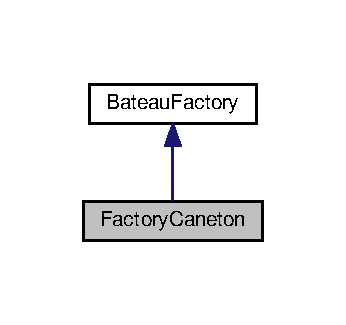
\includegraphics[width=166pt]{classFactoryCaneton__inherit__graph}
\end{center}
\end{figure}


Collaboration diagram for Factory\+Caneton\+:
\nopagebreak
\begin{figure}[H]
\begin{center}
\leavevmode
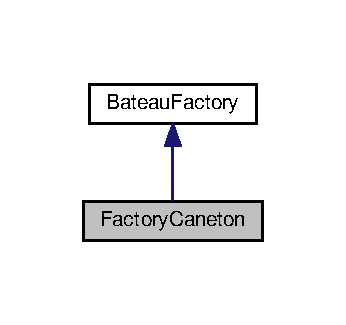
\includegraphics[width=166pt]{classFactoryCaneton__coll__graph}
\end{center}
\end{figure}
\subsection*{Public Member Functions}
\begin{DoxyCompactItemize}
\item 
\hyperlink{classFactoryCaneton_aaf555e37dcffbab41199d886a894fd84}{Factory\+Caneton} ()
\begin{DoxyCompactList}\small\item\em Constructeur. \end{DoxyCompactList}\item 
std\+::shared\+\_\+ptr$<$ \hyperlink{classBateau}{Bateau} $>$ \hyperlink{classFactoryCaneton_ac03710919dab69d816bb4c8fd047f4eb}{creer\+Bateau} ()
\begin{DoxyCompactList}\small\item\em Récupère le \hyperlink{classCaneton}{Caneton} créé \end{DoxyCompactList}\end{DoxyCompactItemize}


\subsection{Detailed Description}
classe representant une usine à \hyperlink{classCaneton}{Caneton} 

La classe modélise une usine à \hyperlink{classBateau}{Bateau} de taille 1 

\subsection{Constructor \& Destructor Documentation}
\hypertarget{classFactoryCaneton_aaf555e37dcffbab41199d886a894fd84}{\index{Factory\+Caneton@{Factory\+Caneton}!Factory\+Caneton@{Factory\+Caneton}}
\index{Factory\+Caneton@{Factory\+Caneton}!Factory\+Caneton@{Factory\+Caneton}}
\subsubsection[{Factory\+Caneton}]{\setlength{\rightskip}{0pt plus 5cm}Factory\+Caneton\+::\+Factory\+Caneton (
\begin{DoxyParamCaption}
{}
\end{DoxyParamCaption}
)}}\label{classFactoryCaneton_aaf555e37dcffbab41199d886a894fd84}


Constructeur. 

Constructeur de la classe \hyperlink{classFactoryCaneton}{Factory\+Caneton} 

\subsection{Member Function Documentation}
\hypertarget{classFactoryCaneton_ac03710919dab69d816bb4c8fd047f4eb}{\index{Factory\+Caneton@{Factory\+Caneton}!creer\+Bateau@{creer\+Bateau}}
\index{creer\+Bateau@{creer\+Bateau}!Factory\+Caneton@{Factory\+Caneton}}
\subsubsection[{creer\+Bateau}]{\setlength{\rightskip}{0pt plus 5cm}shared\+\_\+ptr$<$ {\bf Bateau} $>$ Factory\+Caneton\+::creer\+Bateau (
\begin{DoxyParamCaption}
{}
\end{DoxyParamCaption}
)\hspace{0.3cm}{\ttfamily [virtual]}}}\label{classFactoryCaneton_ac03710919dab69d816bb4c8fd047f4eb}


Récupère le \hyperlink{classCaneton}{Caneton} créé 

Méthode permettant de créer un \hyperlink{classCaneton}{Caneton} et de le récupérer

\begin{DoxyReturn}{Returns}
le \hyperlink{classBateau}{Bateau} de taille 1 
\end{DoxyReturn}


Implements \hyperlink{classBateauFactory_a8cec9c2ab3793cec80e43b3d940da1d9}{Bateau\+Factory}.



The documentation for this class was generated from the following files\+:\begin{DoxyCompactItemize}
\item 
factorycaneton.\+h\item 
factorycaneton.\+cpp\end{DoxyCompactItemize}

\hypertarget{classFactoryCygne}{\section{Factory\+Cygne Class Reference}
\label{classFactoryCygne}\index{Factory\+Cygne@{Factory\+Cygne}}
}


classe representant une usine à \hyperlink{classCygne}{Cygne}  




{\ttfamily \#include $<$factorycygne.\+h$>$}



Inheritance diagram for Factory\+Cygne\+:
\nopagebreak
\begin{figure}[H]
\begin{center}
\leavevmode
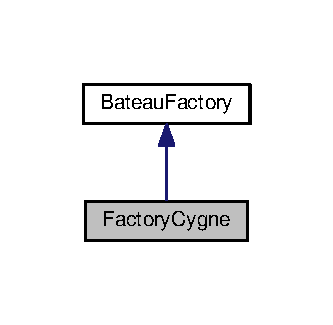
\includegraphics[width=160pt]{classFactoryCygne__inherit__graph}
\end{center}
\end{figure}


Collaboration diagram for Factory\+Cygne\+:
\nopagebreak
\begin{figure}[H]
\begin{center}
\leavevmode
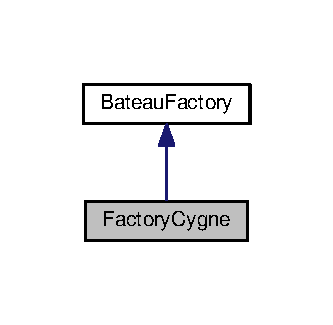
\includegraphics[width=160pt]{classFactoryCygne__coll__graph}
\end{center}
\end{figure}
\subsection*{Public Member Functions}
\begin{DoxyCompactItemize}
\item 
\hyperlink{classFactoryCygne_a976f5ce581e2beb4efd0a1662f2dd377}{Factory\+Cygne} ()
\begin{DoxyCompactList}\small\item\em Constructeur. \end{DoxyCompactList}\item 
std\+::shared\+\_\+ptr$<$ \hyperlink{classBateau}{Bateau} $>$ \hyperlink{classFactoryCygne_aa49b4a3704bcb68c0e31cebc3f5767b8}{creer\+Bateau} ()
\begin{DoxyCompactList}\small\item\em Récupère le \hyperlink{classCygne}{Cygne} créé \end{DoxyCompactList}\end{DoxyCompactItemize}


\subsection{Detailed Description}
classe representant une usine à \hyperlink{classCygne}{Cygne} 

La classe modélise une usine à \hyperlink{classBateau}{Bateau} de taille 4 

\subsection{Constructor \& Destructor Documentation}
\hypertarget{classFactoryCygne_a976f5ce581e2beb4efd0a1662f2dd377}{\index{Factory\+Cygne@{Factory\+Cygne}!Factory\+Cygne@{Factory\+Cygne}}
\index{Factory\+Cygne@{Factory\+Cygne}!Factory\+Cygne@{Factory\+Cygne}}
\subsubsection[{Factory\+Cygne}]{\setlength{\rightskip}{0pt plus 5cm}Factory\+Cygne\+::\+Factory\+Cygne (
\begin{DoxyParamCaption}
{}
\end{DoxyParamCaption}
)}}\label{classFactoryCygne_a976f5ce581e2beb4efd0a1662f2dd377}


Constructeur. 

Constructeur de la classe \hyperlink{classFactoryCygne}{Factory\+Cygne} 

\subsection{Member Function Documentation}
\hypertarget{classFactoryCygne_aa49b4a3704bcb68c0e31cebc3f5767b8}{\index{Factory\+Cygne@{Factory\+Cygne}!creer\+Bateau@{creer\+Bateau}}
\index{creer\+Bateau@{creer\+Bateau}!Factory\+Cygne@{Factory\+Cygne}}
\subsubsection[{creer\+Bateau}]{\setlength{\rightskip}{0pt plus 5cm}shared\+\_\+ptr$<$ {\bf Bateau} $>$ Factory\+Cygne\+::creer\+Bateau (
\begin{DoxyParamCaption}
{}
\end{DoxyParamCaption}
)\hspace{0.3cm}{\ttfamily [virtual]}}}\label{classFactoryCygne_aa49b4a3704bcb68c0e31cebc3f5767b8}


Récupère le \hyperlink{classCygne}{Cygne} créé 

Méthode permettant de créer un \hyperlink{classCygne}{Cygne} et de le récupérer

\begin{DoxyReturn}{Returns}
le \hyperlink{classBateau}{Bateau} de taille 4 
\end{DoxyReturn}


Implements \hyperlink{classBateauFactory_a8cec9c2ab3793cec80e43b3d940da1d9}{Bateau\+Factory}.



The documentation for this class was generated from the following files\+:\begin{DoxyCompactItemize}
\item 
factorycygne.\+h\item 
factorycygne.\+cpp\end{DoxyCompactItemize}

\hypertarget{classFactoryOie}{\section{Factory\+Oie Class Reference}
\label{classFactoryOie}\index{Factory\+Oie@{Factory\+Oie}}
}


classe representant une usine à \hyperlink{classOie}{Oie}  




{\ttfamily \#include $<$factoryoie.\+h$>$}



Inheritance diagram for Factory\+Oie\+:
\nopagebreak
\begin{figure}[H]
\begin{center}
\leavevmode
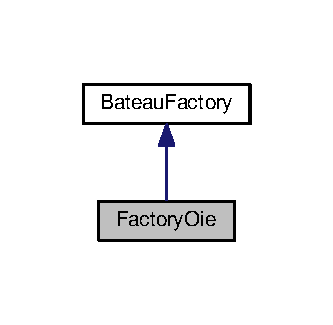
\includegraphics[width=160pt]{classFactoryOie__inherit__graph}
\end{center}
\end{figure}


Collaboration diagram for Factory\+Oie\+:
\nopagebreak
\begin{figure}[H]
\begin{center}
\leavevmode
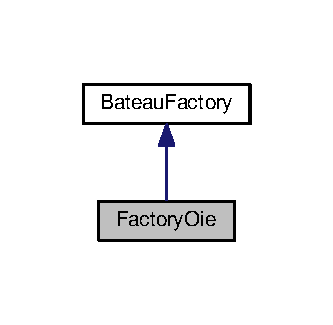
\includegraphics[width=160pt]{classFactoryOie__coll__graph}
\end{center}
\end{figure}
\subsection*{Public Member Functions}
\begin{DoxyCompactItemize}
\item 
\hyperlink{classFactoryOie_a7dee7f5177dd996e37ab8d31d4f5188b}{Factory\+Oie} ()
\begin{DoxyCompactList}\small\item\em Constructeur. \end{DoxyCompactList}\item 
std\+::shared\+\_\+ptr$<$ \hyperlink{classBateau}{Bateau} $>$ \hyperlink{classFactoryOie_aef35f008954feedb26821fdf5b73328f}{creer\+Bateau} ()
\begin{DoxyCompactList}\small\item\em Récupère le \hyperlink{classOie}{Oie} créé \end{DoxyCompactList}\end{DoxyCompactItemize}


\subsection{Detailed Description}
classe representant une usine à \hyperlink{classOie}{Oie} 

La classe modélise une usine à \hyperlink{classBateau}{Bateau} de taille 3 

\subsection{Constructor \& Destructor Documentation}
\hypertarget{classFactoryOie_a7dee7f5177dd996e37ab8d31d4f5188b}{\index{Factory\+Oie@{Factory\+Oie}!Factory\+Oie@{Factory\+Oie}}
\index{Factory\+Oie@{Factory\+Oie}!Factory\+Oie@{Factory\+Oie}}
\subsubsection[{Factory\+Oie}]{\setlength{\rightskip}{0pt plus 5cm}Factory\+Oie\+::\+Factory\+Oie (
\begin{DoxyParamCaption}
{}
\end{DoxyParamCaption}
)}}\label{classFactoryOie_a7dee7f5177dd996e37ab8d31d4f5188b}


Constructeur. 

Constructeur de la classe \hyperlink{classFactoryOie}{Factory\+Oie} 

\subsection{Member Function Documentation}
\hypertarget{classFactoryOie_aef35f008954feedb26821fdf5b73328f}{\index{Factory\+Oie@{Factory\+Oie}!creer\+Bateau@{creer\+Bateau}}
\index{creer\+Bateau@{creer\+Bateau}!Factory\+Oie@{Factory\+Oie}}
\subsubsection[{creer\+Bateau}]{\setlength{\rightskip}{0pt plus 5cm}shared\+\_\+ptr$<$ {\bf Bateau} $>$ Factory\+Oie\+::creer\+Bateau (
\begin{DoxyParamCaption}
{}
\end{DoxyParamCaption}
)\hspace{0.3cm}{\ttfamily [virtual]}}}\label{classFactoryOie_aef35f008954feedb26821fdf5b73328f}


Récupère le \hyperlink{classOie}{Oie} créé 

Méthode permettant de créer un \hyperlink{classOie}{Oie} et de le récupérer

\begin{DoxyReturn}{Returns}
le \hyperlink{classBateau}{Bateau} de taille 3 
\end{DoxyReturn}


Implements \hyperlink{classBateauFactory_a8cec9c2ab3793cec80e43b3d940da1d9}{Bateau\+Factory}.



The documentation for this class was generated from the following files\+:\begin{DoxyCompactItemize}
\item 
factoryoie.\+h\item 
factoryoie.\+cpp\end{DoxyCompactItemize}

\hypertarget{classIAffichage}{\section{I\+Affichage Interface Reference}
\label{classIAffichage}\index{I\+Affichage@{I\+Affichage}}
}


classe representant les comportements des affichages  




{\ttfamily \#include $<$iaffichage.\+h$>$}



Inheritance diagram for I\+Affichage\+:
\nopagebreak
\begin{figure}[H]
\begin{center}
\leavevmode
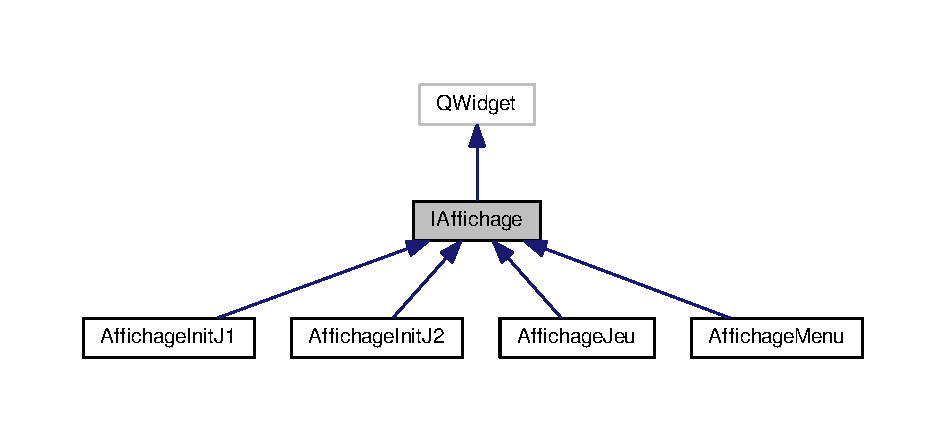
\includegraphics[width=350pt]{classIAffichage__inherit__graph}
\end{center}
\end{figure}


Collaboration diagram for I\+Affichage\+:
\nopagebreak
\begin{figure}[H]
\begin{center}
\leavevmode
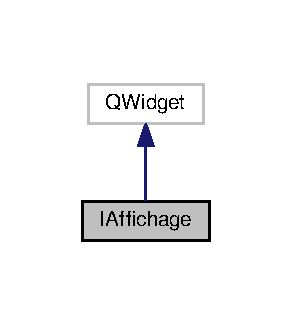
\includegraphics[width=140pt]{classIAffichage__coll__graph}
\end{center}
\end{figure}
\subsection*{Public Member Functions}
\begin{DoxyCompactItemize}
\item 
\hypertarget{classIAffichage_a0bc54bcf0afae03db411636834b372fe}{\hyperlink{classIAffichage_a0bc54bcf0afae03db411636834b372fe}{I\+Affichage} ()}\label{classIAffichage_a0bc54bcf0afae03db411636834b372fe}

\begin{DoxyCompactList}\small\item\em Constructeur Constructeur de la classe \hyperlink{classIAffichage}{I\+Affichage}. \end{DoxyCompactList}\item 
virtual void \hyperlink{classIAffichage_a87e168995340186305675343d4b769fe}{afficher} ()=0
\begin{DoxyCompactList}\small\item\em Affiche la fenêtre. \end{DoxyCompactList}\item 
virtual void \hyperlink{classIAffichage_a147a42f3068b7dc51d5a196252e53a39}{change\+To\+Menu} ()=0
\begin{DoxyCompactList}\small\item\em Change la fenêtre vers le menu. \end{DoxyCompactList}\item 
virtual void \hyperlink{classIAffichage_ac03c56ab489b760b1e42af15ac421039}{change\+To\+Initialisation\+J1} ()=0
\begin{DoxyCompactList}\small\item\em Change la fenêtre vers l'initialisation pour le J1. \end{DoxyCompactList}\item 
virtual void \hyperlink{classIAffichage_a425bcafe36ba332f2cbc4badc99e19c2}{change\+To\+Initialisation\+J2} ()=0
\begin{DoxyCompactList}\small\item\em Change la fenêtre vers l'initialisation pour le J2. \end{DoxyCompactList}\item 
virtual void \hyperlink{classIAffichage_a52e20907ed94e272c592429d95fa5165}{change\+To\+Jeu} ()=0
\begin{DoxyCompactList}\small\item\em Change la fenêtre vers le jeu. \end{DoxyCompactList}\item 
std\+::shared\+\_\+ptr$<$ \hyperlink{classCore}{Core} $>$ \hyperlink{classIAffichage_a7245173f805ffb6a17b4fbda887bcfd6}{get\+Core} ()
\begin{DoxyCompactList}\small\item\em Récupère le core de l'application. \end{DoxyCompactList}\item 
\hypertarget{classIAffichage_a2b22d88915d1a8951ba3cd027bbaed0f}{virtual \hyperlink{classIAffichage_a2b22d88915d1a8951ba3cd027bbaed0f}{$\sim$\+I\+Affichage} ()}\label{classIAffichage_a2b22d88915d1a8951ba3cd027bbaed0f}

\begin{DoxyCompactList}\small\item\em Destructeur Destructeur de la classe \hyperlink{classIAffichage}{I\+Affichage}. \end{DoxyCompactList}\end{DoxyCompactItemize}
\subsection*{Protected Attributes}
\begin{DoxyCompactItemize}
\item 
std\+::shared\+\_\+ptr$<$ \hyperlink{classCore}{Core} $>$ \hyperlink{classIAffichage_ad1ae8f669e8aec4035c383bd640c5a81}{core\+\_\+}
\end{DoxyCompactItemize}


\subsection{Detailed Description}
classe representant les comportements des affichages 

La classe modélise les comportements des affichages de jeu, des initialisations, ... 

\subsection{Member Function Documentation}
\hypertarget{classIAffichage_a87e168995340186305675343d4b769fe}{\index{I\+Affichage@{I\+Affichage}!afficher@{afficher}}
\index{afficher@{afficher}!I\+Affichage@{I\+Affichage}}
\subsubsection[{afficher}]{\setlength{\rightskip}{0pt plus 5cm}virtual void I\+Affichage\+::afficher (
\begin{DoxyParamCaption}
{}
\end{DoxyParamCaption}
)\hspace{0.3cm}{\ttfamily [pure virtual]}}}\label{classIAffichage_a87e168995340186305675343d4b769fe}


Affiche la fenêtre. 

Méthode pour afficher la fenêtre 

Implemented in \hyperlink{classAffichageMenu_abec0adf6db92df26a937ff702a5a87fc}{Affichage\+Menu}, \hyperlink{classAffichageJeu_a29d9ad7ef0161faa698bd0850efbb1fc}{Affichage\+Jeu}, \hyperlink{classAffichageInitJ1_a469000a4072c712f88ee75ed6cc03d3b}{Affichage\+Init\+J1}, and \hyperlink{classAffichageInitJ2_a4b5dbe3833780c14aaaf946a7542e085}{Affichage\+Init\+J2}.

\hypertarget{classIAffichage_ac03c56ab489b760b1e42af15ac421039}{\index{I\+Affichage@{I\+Affichage}!change\+To\+Initialisation\+J1@{change\+To\+Initialisation\+J1}}
\index{change\+To\+Initialisation\+J1@{change\+To\+Initialisation\+J1}!I\+Affichage@{I\+Affichage}}
\subsubsection[{change\+To\+Initialisation\+J1}]{\setlength{\rightskip}{0pt plus 5cm}virtual void I\+Affichage\+::change\+To\+Initialisation\+J1 (
\begin{DoxyParamCaption}
{}
\end{DoxyParamCaption}
)\hspace{0.3cm}{\ttfamily [pure virtual]}}}\label{classIAffichage_ac03c56ab489b760b1e42af15ac421039}


Change la fenêtre vers l'initialisation pour le J1. 

Méthode pour switcher la fenêtre courante avec celle de l'initialisation du J1 

Implemented in \hyperlink{classAffichageJeu_a4e8693c20861bc9e79e0c0037ba4ffa8}{Affichage\+Jeu}, \hyperlink{classAffichageMenu_ab7df249dc5db82d25613b80c28ba1ed4}{Affichage\+Menu}, \hyperlink{classAffichageInitJ1_a07ee576320b2bd22733ac142fd10b14c}{Affichage\+Init\+J1}, and \hyperlink{classAffichageInitJ2_a355056fd45cd18a199801eaf20181edc}{Affichage\+Init\+J2}.

\hypertarget{classIAffichage_a425bcafe36ba332f2cbc4badc99e19c2}{\index{I\+Affichage@{I\+Affichage}!change\+To\+Initialisation\+J2@{change\+To\+Initialisation\+J2}}
\index{change\+To\+Initialisation\+J2@{change\+To\+Initialisation\+J2}!I\+Affichage@{I\+Affichage}}
\subsubsection[{change\+To\+Initialisation\+J2}]{\setlength{\rightskip}{0pt plus 5cm}virtual void I\+Affichage\+::change\+To\+Initialisation\+J2 (
\begin{DoxyParamCaption}
{}
\end{DoxyParamCaption}
)\hspace{0.3cm}{\ttfamily [pure virtual]}}}\label{classIAffichage_a425bcafe36ba332f2cbc4badc99e19c2}


Change la fenêtre vers l'initialisation pour le J2. 

Méthode pour switcher la fenêtre courante avec celle de l'initialisation du J2 

Implemented in \hyperlink{classAffichageJeu_a62db45f512fb855b096bcfd19e379429}{Affichage\+Jeu}, \hyperlink{classAffichageMenu_a1980bc54a6156938cc3b737972facd32}{Affichage\+Menu}, \hyperlink{classAffichageInitJ2_a7f861d5e94c8ff21aae5b05601678292}{Affichage\+Init\+J2}, and \hyperlink{classAffichageInitJ1_ad1f6286f0aa162fec476d69049a2c1a8}{Affichage\+Init\+J1}.

\hypertarget{classIAffichage_a52e20907ed94e272c592429d95fa5165}{\index{I\+Affichage@{I\+Affichage}!change\+To\+Jeu@{change\+To\+Jeu}}
\index{change\+To\+Jeu@{change\+To\+Jeu}!I\+Affichage@{I\+Affichage}}
\subsubsection[{change\+To\+Jeu}]{\setlength{\rightskip}{0pt plus 5cm}virtual void I\+Affichage\+::change\+To\+Jeu (
\begin{DoxyParamCaption}
{}
\end{DoxyParamCaption}
)\hspace{0.3cm}{\ttfamily [pure virtual]}}}\label{classIAffichage_a52e20907ed94e272c592429d95fa5165}


Change la fenêtre vers le jeu. 

Méthode pour switcher la fenêtre courante avec celle du jeu 

Implemented in \hyperlink{classAffichageJeu_aec00eea36f08e0bd187832d17ec32680}{Affichage\+Jeu}, \hyperlink{classAffichageMenu_a878a89a1ce7e138695e3e5fde5e020af}{Affichage\+Menu}, \hyperlink{classAffichageInitJ1_a4fcbe1401407498fc32e5cedf797a9e4}{Affichage\+Init\+J1}, and \hyperlink{classAffichageInitJ2_ab2af503532ad81094f890d887bdb4f23}{Affichage\+Init\+J2}.

\hypertarget{classIAffichage_a147a42f3068b7dc51d5a196252e53a39}{\index{I\+Affichage@{I\+Affichage}!change\+To\+Menu@{change\+To\+Menu}}
\index{change\+To\+Menu@{change\+To\+Menu}!I\+Affichage@{I\+Affichage}}
\subsubsection[{change\+To\+Menu}]{\setlength{\rightskip}{0pt plus 5cm}virtual void I\+Affichage\+::change\+To\+Menu (
\begin{DoxyParamCaption}
{}
\end{DoxyParamCaption}
)\hspace{0.3cm}{\ttfamily [pure virtual]}}}\label{classIAffichage_a147a42f3068b7dc51d5a196252e53a39}


Change la fenêtre vers le menu. 

Méthode pour switcher la fenêtre courante avec celle du menu 

Implemented in \hyperlink{classAffichageJeu_aa0fe30f907b9c0c2007466d287c701fd}{Affichage\+Jeu}, \hyperlink{classAffichageMenu_a5f825906a1c5afccfbb03b007906bd28}{Affichage\+Menu}, \hyperlink{classAffichageInitJ1_ac579f8933a11bc3e49923d414b20acab}{Affichage\+Init\+J1}, and \hyperlink{classAffichageInitJ2_a7266e6ce2188930080dc3ede1322d14d}{Affichage\+Init\+J2}.

\hypertarget{classIAffichage_a7245173f805ffb6a17b4fbda887bcfd6}{\index{I\+Affichage@{I\+Affichage}!get\+Core@{get\+Core}}
\index{get\+Core@{get\+Core}!I\+Affichage@{I\+Affichage}}
\subsubsection[{get\+Core}]{\setlength{\rightskip}{0pt plus 5cm}shared\+\_\+ptr$<$ {\bf Core} $>$ I\+Affichage\+::get\+Core (
\begin{DoxyParamCaption}
{}
\end{DoxyParamCaption}
)}}\label{classIAffichage_a7245173f805ffb6a17b4fbda887bcfd6}


Récupère le core de l'application. 

Méthode pour récupérer le core de l'application

\begin{DoxyReturn}{Returns}
le core de l'application 
\end{DoxyReturn}


\subsection{Member Data Documentation}
\hypertarget{classIAffichage_ad1ae8f669e8aec4035c383bd640c5a81}{\index{I\+Affichage@{I\+Affichage}!core\+\_\+@{core\+\_\+}}
\index{core\+\_\+@{core\+\_\+}!I\+Affichage@{I\+Affichage}}
\subsubsection[{core\+\_\+}]{\setlength{\rightskip}{0pt plus 5cm}std\+::shared\+\_\+ptr$<${\bf Core}$>$ I\+Affichage\+::core\+\_\+\hspace{0.3cm}{\ttfamily [protected]}}}\label{classIAffichage_ad1ae8f669e8aec4035c383bd640c5a81}
le core de l'application 

The documentation for this interface was generated from the following files\+:\begin{DoxyCompactItemize}
\item 
iaffichage.\+h\item 
iaffichage.\+cpp\end{DoxyCompactItemize}

\hypertarget{classMer}{\section{Mer Class Reference}
\label{classMer}\index{Mer@{Mer}}
}


classe representant de la \hyperlink{classMer}{Mer}  




{\ttfamily \#include $<$mer.\+h$>$}



Inheritance diagram for Mer\+:
\nopagebreak
\begin{figure}[H]
\begin{center}
\leavevmode
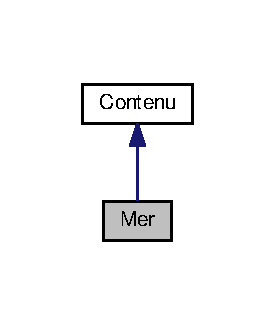
\includegraphics[width=132pt]{classMer__inherit__graph}
\end{center}
\end{figure}


Collaboration diagram for Mer\+:
\nopagebreak
\begin{figure}[H]
\begin{center}
\leavevmode
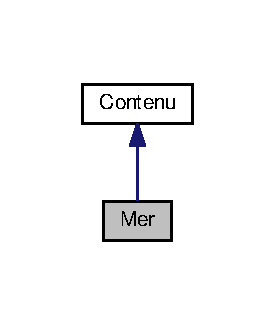
\includegraphics[width=132pt]{classMer__coll__graph}
\end{center}
\end{figure}
\subsection*{Public Member Functions}
\begin{DoxyCompactItemize}
\item 
\hyperlink{classMer_ace88286368f6f30f2462de952083bcd0}{Mer} ()
\begin{DoxyCompactList}\small\item\em Constructeur. \end{DoxyCompactList}\item 
bool \hyperlink{classMer_aa30fffa94a8e0d5be6ae503aa8392973}{action} (\hyperlink{classCase}{Case} $\ast$c)
\begin{DoxyCompactList}\small\item\em Action émise lorsqu'on a cliqué sur une case contenant de la \hyperlink{classMer}{Mer}. \end{DoxyCompactList}\item 
void \hyperlink{classMer_ab20617d436898cc631fc1842e897de0c}{set\+X} (int x)
\begin{DoxyCompactList}\small\item\em Modifie la coordonnée X de la \hyperlink{classMer}{Mer}. \end{DoxyCompactList}\item 
void \hyperlink{classMer_a13ac62cb31e498d5bcf786d5a0d196ed}{set\+Y} (int y)
\begin{DoxyCompactList}\small\item\em Modifie la coordonnée Y de la \hyperlink{classMer}{Mer}. \end{DoxyCompactList}\item 
void \hyperlink{classMer_a3244c63c7b077ef84e593d9b5e5f4472}{set\+Horizontal} (bool a)
\begin{DoxyCompactList}\small\item\em Modifie l'orientation de la \hyperlink{classMer}{Mer}. \end{DoxyCompactList}\item 
int \hyperlink{classMer_a668a9c3acfa903bb7c8e1d607e1229a4}{get\+X} ()
\begin{DoxyCompactList}\small\item\em Récupère la ligne où se trouve la \hyperlink{classMer}{Mer}. \end{DoxyCompactList}\item 
int \hyperlink{classMer_a41f5d00f824057af9c9b57d666bf6fcc}{get\+Y} ()
\begin{DoxyCompactList}\small\item\em Récupère la colonne où se trouve la \hyperlink{classMer}{Mer}. \end{DoxyCompactList}\item 
bool \hyperlink{classMer_aa2cfaf3bb10d817c535b843724759bc7}{get\+Horizontal} ()
\begin{DoxyCompactList}\small\item\em Récupère l'orientation de la \hyperlink{classMer}{Mer}. \end{DoxyCompactList}\item 
int \hyperlink{classMer_ad3662e679f566da98a77b585d1699a7e}{get\+Taille} ()
\begin{DoxyCompactList}\small\item\em Connaitre la taille de la \hyperlink{classMer}{Mer}. \end{DoxyCompactList}\item 
bool \hyperlink{classMer_ac76c2299715ae08f07e8a9fc0821b032}{is\+Empty} ()
\begin{DoxyCompactList}\small\item\em Savoir si le contenu est vide. \end{DoxyCompactList}\item 
bool \hyperlink{classMer_a2ec6ecba14a8f737335720f3dffe9877}{touche} ()
\begin{DoxyCompactList}\small\item\em Savoir si le \hyperlink{classContenu}{Contenu} est touché \end{DoxyCompactList}\item 
bool \hyperlink{classMer_aa1a5b5633f2d7590e3074bf70a867ee0}{est\+Coule} ()
\begin{DoxyCompactList}\small\item\em Savoir si le \hyperlink{classContenu}{Contenu} est coulé \end{DoxyCompactList}\item 
\hypertarget{classMer_a5c47272a53feac903046599b3c638d2c}{virtual \hyperlink{classMer_a5c47272a53feac903046599b3c638d2c}{$\sim$\+Mer} ()}\label{classMer_a5c47272a53feac903046599b3c638d2c}

\begin{DoxyCompactList}\small\item\em Destructeur Destructeur de la classe \hyperlink{classMer}{Mer}. \end{DoxyCompactList}\end{DoxyCompactItemize}
\subsection*{Additional Inherited Members}


\subsection{Detailed Description}
classe representant de la \hyperlink{classMer}{Mer} 

La classe gère l'ensemble des actions impactant une \hyperlink{classMer}{Mer} 

\subsection{Constructor \& Destructor Documentation}
\hypertarget{classMer_ace88286368f6f30f2462de952083bcd0}{\index{Mer@{Mer}!Mer@{Mer}}
\index{Mer@{Mer}!Mer@{Mer}}
\subsubsection[{Mer}]{\setlength{\rightskip}{0pt plus 5cm}Mer\+::\+Mer (
\begin{DoxyParamCaption}
{}
\end{DoxyParamCaption}
)}}\label{classMer_ace88286368f6f30f2462de952083bcd0}


Constructeur. 

Constructeur de la classe \hyperlink{classMer}{Mer} 

\subsection{Member Function Documentation}
\hypertarget{classMer_aa30fffa94a8e0d5be6ae503aa8392973}{\index{Mer@{Mer}!action@{action}}
\index{action@{action}!Mer@{Mer}}
\subsubsection[{action}]{\setlength{\rightskip}{0pt plus 5cm}bool Mer\+::action (
\begin{DoxyParamCaption}
\item[{{\bf Case} $\ast$}]{c}
\end{DoxyParamCaption}
)\hspace{0.3cm}{\ttfamily [virtual]}}}\label{classMer_aa30fffa94a8e0d5be6ae503aa8392973}


Action émise lorsqu'on a cliqué sur une case contenant de la \hyperlink{classMer}{Mer}. 

Méthode permettant de savoir si le contenu de la case est de la \hyperlink{classMer}{Mer}


\begin{DoxyParams}{Parameters}
{\em c} & \+: la case sur laquelle on a cliqué\\
\hline
\end{DoxyParams}
\begin{DoxyReturn}{Returns}
false si le contenu de la case est de la \hyperlink{classMer}{Mer} sinon true 
\end{DoxyReturn}


Implements \hyperlink{classContenu_ae54145207bfdae5a24ce2c8c523c74a0}{Contenu}.

\hypertarget{classMer_aa1a5b5633f2d7590e3074bf70a867ee0}{\index{Mer@{Mer}!est\+Coule@{est\+Coule}}
\index{est\+Coule@{est\+Coule}!Mer@{Mer}}
\subsubsection[{est\+Coule}]{\setlength{\rightskip}{0pt plus 5cm}bool Mer\+::est\+Coule (
\begin{DoxyParamCaption}
{}
\end{DoxyParamCaption}
)\hspace{0.3cm}{\ttfamily [virtual]}}}\label{classMer_aa1a5b5633f2d7590e3074bf70a867ee0}


Savoir si le \hyperlink{classContenu}{Contenu} est coulé 

Méthode permettant de savoir si le contenu de la case est coulé logique dans ce cas

\begin{DoxyReturn}{Returns}
false ici 
\end{DoxyReturn}


Implements \hyperlink{classContenu_ad8ba918a8d5a08e4f8c0c742778500d6}{Contenu}.

\hypertarget{classMer_aa2cfaf3bb10d817c535b843724759bc7}{\index{Mer@{Mer}!get\+Horizontal@{get\+Horizontal}}
\index{get\+Horizontal@{get\+Horizontal}!Mer@{Mer}}
\subsubsection[{get\+Horizontal}]{\setlength{\rightskip}{0pt plus 5cm}bool Mer\+::get\+Horizontal (
\begin{DoxyParamCaption}
{}
\end{DoxyParamCaption}
)\hspace{0.3cm}{\ttfamily [virtual]}}}\label{classMer_aa2cfaf3bb10d817c535b843724759bc7}


Récupère l'orientation de la \hyperlink{classMer}{Mer}. 

Méthode permettant de savoir si la \hyperlink{classMer}{Mer} est horizontal ou vertical

\begin{DoxyReturn}{Returns}
true si la \hyperlink{classMer}{Mer} est horizontal, false sinon 
\end{DoxyReturn}


Implements \hyperlink{classContenu_aa9b4dbb3de416310cd53422a0d14879b}{Contenu}.

\hypertarget{classMer_ad3662e679f566da98a77b585d1699a7e}{\index{Mer@{Mer}!get\+Taille@{get\+Taille}}
\index{get\+Taille@{get\+Taille}!Mer@{Mer}}
\subsubsection[{get\+Taille}]{\setlength{\rightskip}{0pt plus 5cm}int Mer\+::get\+Taille (
\begin{DoxyParamCaption}
{}
\end{DoxyParamCaption}
)\hspace{0.3cm}{\ttfamily [virtual]}}}\label{classMer_ad3662e679f566da98a77b585d1699a7e}


Connaitre la taille de la \hyperlink{classMer}{Mer}. 

Méthode permettant de connaitre la taille de la \hyperlink{classMer}{Mer}

\begin{DoxyReturn}{Returns}
la taille de la \hyperlink{classMer}{Mer} (1) 
\end{DoxyReturn}


Implements \hyperlink{classContenu_abba99a1726eb744067cca7deb571444b}{Contenu}.

\hypertarget{classMer_a668a9c3acfa903bb7c8e1d607e1229a4}{\index{Mer@{Mer}!get\+X@{get\+X}}
\index{get\+X@{get\+X}!Mer@{Mer}}
\subsubsection[{get\+X}]{\setlength{\rightskip}{0pt plus 5cm}int Mer\+::get\+X (
\begin{DoxyParamCaption}
{}
\end{DoxyParamCaption}
)\hspace{0.3cm}{\ttfamily [virtual]}}}\label{classMer_a668a9c3acfa903bb7c8e1d607e1229a4}


Récupère la ligne où se trouve la \hyperlink{classMer}{Mer}. 

Méthode permettant de récupérer la ligne sur laquelle se situe la \hyperlink{classMer}{Mer} sur la carte

\begin{DoxyReturn}{Returns}
le numéro de ligne sur laquelle se trouve la \hyperlink{classMer}{Mer} 
\end{DoxyReturn}


Implements \hyperlink{classContenu_afce83627ee635c60edb0edced8191af4}{Contenu}.

\hypertarget{classMer_a41f5d00f824057af9c9b57d666bf6fcc}{\index{Mer@{Mer}!get\+Y@{get\+Y}}
\index{get\+Y@{get\+Y}!Mer@{Mer}}
\subsubsection[{get\+Y}]{\setlength{\rightskip}{0pt plus 5cm}int Mer\+::get\+Y (
\begin{DoxyParamCaption}
{}
\end{DoxyParamCaption}
)\hspace{0.3cm}{\ttfamily [virtual]}}}\label{classMer_a41f5d00f824057af9c9b57d666bf6fcc}


Récupère la colonne où se trouve la \hyperlink{classMer}{Mer}. 

Méthode permettant de récupérer la colonne sur laquelle se situe la \hyperlink{classMer}{Mer} sur la carte

\begin{DoxyReturn}{Returns}
le numéro de colonne sur laquelle se trouve la \hyperlink{classMer}{Mer} 
\end{DoxyReturn}


Implements \hyperlink{classContenu_a1087d1609ec4842bb3d2a5dd960359b6}{Contenu}.

\hypertarget{classMer_ac76c2299715ae08f07e8a9fc0821b032}{\index{Mer@{Mer}!is\+Empty@{is\+Empty}}
\index{is\+Empty@{is\+Empty}!Mer@{Mer}}
\subsubsection[{is\+Empty}]{\setlength{\rightskip}{0pt plus 5cm}bool Mer\+::is\+Empty (
\begin{DoxyParamCaption}
{}
\end{DoxyParamCaption}
)\hspace{0.3cm}{\ttfamily [virtual]}}}\label{classMer_ac76c2299715ae08f07e8a9fc0821b032}


Savoir si le contenu est vide. 

Méthode permettant de savoir si le contenu est vide

\begin{DoxyReturn}{Returns}
false 
\end{DoxyReturn}


Implements \hyperlink{classContenu_a426053a6e632f1963c1c59c1515c99fb}{Contenu}.

\hypertarget{classMer_a3244c63c7b077ef84e593d9b5e5f4472}{\index{Mer@{Mer}!set\+Horizontal@{set\+Horizontal}}
\index{set\+Horizontal@{set\+Horizontal}!Mer@{Mer}}
\subsubsection[{set\+Horizontal}]{\setlength{\rightskip}{0pt plus 5cm}void Mer\+::set\+Horizontal (
\begin{DoxyParamCaption}
\item[{bool}]{a}
\end{DoxyParamCaption}
)\hspace{0.3cm}{\ttfamily [virtual]}}}\label{classMer_a3244c63c7b077ef84e593d9b5e5f4472}


Modifie l'orientation de la \hyperlink{classMer}{Mer}. 

Méthode permettant de modifier l'orientation de la \hyperlink{classMer}{Mer}


\begin{DoxyParams}{Parameters}
{\em a} & \+: booléen à true \+: horizontal, sinon vertical \\
\hline
\end{DoxyParams}


Implements \hyperlink{classContenu_ad06f3204769fdc758a5859fbb7cac637}{Contenu}.

\hypertarget{classMer_ab20617d436898cc631fc1842e897de0c}{\index{Mer@{Mer}!set\+X@{set\+X}}
\index{set\+X@{set\+X}!Mer@{Mer}}
\subsubsection[{set\+X}]{\setlength{\rightskip}{0pt plus 5cm}void Mer\+::set\+X (
\begin{DoxyParamCaption}
\item[{int}]{x}
\end{DoxyParamCaption}
)\hspace{0.3cm}{\ttfamily [virtual]}}}\label{classMer_ab20617d436898cc631fc1842e897de0c}


Modifie la coordonnée X de la \hyperlink{classMer}{Mer}. 

Méthode permettant de modifier la coordonnée en X, c'est à dire sur quelle ligne placer la \hyperlink{classMer}{Mer}


\begin{DoxyParams}{Parameters}
{\em x} & \+: numéro de la ligne \\
\hline
\end{DoxyParams}


Implements \hyperlink{classContenu_a801fc9cb327750d2889ab3e7b185c029}{Contenu}.

\hypertarget{classMer_a13ac62cb31e498d5bcf786d5a0d196ed}{\index{Mer@{Mer}!set\+Y@{set\+Y}}
\index{set\+Y@{set\+Y}!Mer@{Mer}}
\subsubsection[{set\+Y}]{\setlength{\rightskip}{0pt plus 5cm}void Mer\+::set\+Y (
\begin{DoxyParamCaption}
\item[{int}]{y}
\end{DoxyParamCaption}
)\hspace{0.3cm}{\ttfamily [virtual]}}}\label{classMer_a13ac62cb31e498d5bcf786d5a0d196ed}


Modifie la coordonnée Y de la \hyperlink{classMer}{Mer}. 

Méthode permettant de modifier la coordonnée en Y, c'est à dire sur quelle colonne placer la \hyperlink{classMer}{Mer}


\begin{DoxyParams}{Parameters}
{\em x} & \+: numéro de la colonne \\
\hline
\end{DoxyParams}


Implements \hyperlink{classContenu_afc6fc6f669313fe77ca57559475d1750}{Contenu}.

\hypertarget{classMer_a2ec6ecba14a8f737335720f3dffe9877}{\index{Mer@{Mer}!touche@{touche}}
\index{touche@{touche}!Mer@{Mer}}
\subsubsection[{touche}]{\setlength{\rightskip}{0pt plus 5cm}bool Mer\+::touche (
\begin{DoxyParamCaption}
{}
\end{DoxyParamCaption}
)\hspace{0.3cm}{\ttfamily [virtual]}}}\label{classMer_a2ec6ecba14a8f737335720f3dffe9877}


Savoir si le \hyperlink{classContenu}{Contenu} est touché 

Méthode permettant de savoir si le \hyperlink{classContenu}{Contenu} est touché

\begin{DoxyReturn}{Returns}
false 
\end{DoxyReturn}


Implements \hyperlink{classContenu_af917356550ccc6025373c652b6e8b938}{Contenu}.



The documentation for this class was generated from the following files\+:\begin{DoxyCompactItemize}
\item 
mer.\+h\item 
mer.\+cpp\end{DoxyCompactItemize}

\hypertarget{classMode1vs1}{\section{Mode1vs1 Class Reference}
\label{classMode1vs1}\index{Mode1vs1@{Mode1vs1}}
}


classe representant le mode de jeu 1\+V\+S1  




{\ttfamily \#include $<$mode1vs1.\+h$>$}



Inheritance diagram for Mode1vs1\+:
\nopagebreak
\begin{figure}[H]
\begin{center}
\leavevmode
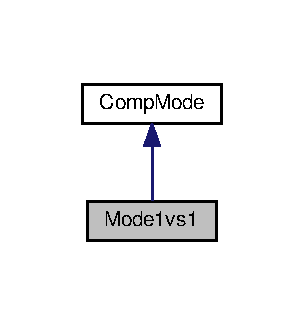
\includegraphics[width=146pt]{classMode1vs1__inherit__graph}
\end{center}
\end{figure}


Collaboration diagram for Mode1vs1\+:
\nopagebreak
\begin{figure}[H]
\begin{center}
\leavevmode
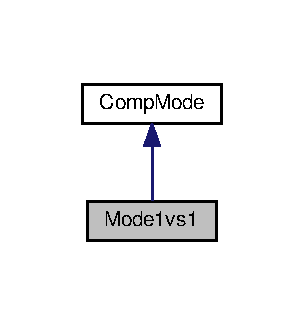
\includegraphics[width=146pt]{classMode1vs1__coll__graph}
\end{center}
\end{figure}
\subsection*{Public Member Functions}
\begin{DoxyCompactItemize}
\item 
\hyperlink{classMode1vs1_aea3b243976c6b47ecaf1b2fd6181cd83}{Mode1vs1} ()
\begin{DoxyCompactList}\small\item\em Constructeur. \end{DoxyCompactList}\item 
void \hyperlink{classMode1vs1_a7e38b115b83c63fe95a0fd96594c6fd9}{get\+Mode} ()
\begin{DoxyCompactList}\small\item\em Décrit le mode dans lequel on est. \end{DoxyCompactList}\item 
void \hyperlink{classMode1vs1_a96b5ffac518dc015717e361248715e78}{initialiser} ()
\begin{DoxyCompactList}\small\item\em Initialiser la carte d'initialisation. \end{DoxyCompactList}\item 
void \hyperlink{classMode1vs1_a4b62821aec55d3a01257eb9cf3d4fd28}{lancer} ()
\begin{DoxyCompactList}\small\item\em Indiquer lorsque le J2 a fini d'initialiser sa carte. \end{DoxyCompactList}\item 
void \hyperlink{classMode1vs1_a21a9f0c6705700943538ce86ec252ad6}{fin\+Init\+J1} ()
\begin{DoxyCompactList}\small\item\em Indiquer lorsque le J1 a fini d'initialiser sa carte. \end{DoxyCompactList}\item 
void \hyperlink{classMode1vs1_ac79db87b0b4a3c72ebf6300ed708c40d}{jouer} ()
\begin{DoxyCompactList}\small\item\em Jouer pour le mode 1\+V\+S1. \end{DoxyCompactList}\item 
void \hyperlink{classMode1vs1_ac94642f3b6ca6b835ded37ed3e2fbf79}{touche} ()
\begin{DoxyCompactList}\small\item\em Action produit après avoir touché un bateau. \end{DoxyCompactList}\item 
void \hyperlink{classMode1vs1_a24bb0744c4614af97c4e983b943a0360}{set\+Affichage} (std\+::shared\+\_\+ptr$<$ \hyperlink{classIAffichage}{I\+Affichage} $>$ aff)
\begin{DoxyCompactList}\small\item\em Permet de changer l'affichage actif. \end{DoxyCompactList}\item 
void \hyperlink{classMode1vs1_a031055c6d9efcc1dd3249c9396f9b496}{choix\+Pour\+J2} ()
\begin{DoxyCompactList}\small\item\em Action produit pour le J2. \end{DoxyCompactList}\item 
\hypertarget{classMode1vs1_abee442099dbc7bbaba244498e8e3406f}{virtual \hyperlink{classMode1vs1_abee442099dbc7bbaba244498e8e3406f}{$\sim$\+Mode1vs1} ()}\label{classMode1vs1_abee442099dbc7bbaba244498e8e3406f}

\begin{DoxyCompactList}\small\item\em Destructeur Destructeur de la classe \hyperlink{classMode1vs1}{Mode1vs1}. \end{DoxyCompactList}\end{DoxyCompactItemize}
\subsection*{Additional Inherited Members}


\subsection{Detailed Description}
classe representant le mode de jeu 1\+V\+S1 

La classe décrit les comportements pour le mode de jeu 1\+V\+S1 

\subsection{Constructor \& Destructor Documentation}
\hypertarget{classMode1vs1_aea3b243976c6b47ecaf1b2fd6181cd83}{\index{Mode1vs1@{Mode1vs1}!Mode1vs1@{Mode1vs1}}
\index{Mode1vs1@{Mode1vs1}!Mode1vs1@{Mode1vs1}}
\subsubsection[{Mode1vs1}]{\setlength{\rightskip}{0pt plus 5cm}Mode1vs1\+::\+Mode1vs1 (
\begin{DoxyParamCaption}
{}
\end{DoxyParamCaption}
)}}\label{classMode1vs1_aea3b243976c6b47ecaf1b2fd6181cd83}


Constructeur. 

Constructeur de la classe \hyperlink{classMode1vs1}{Mode1vs1} 

\subsection{Member Function Documentation}
\hypertarget{classMode1vs1_a031055c6d9efcc1dd3249c9396f9b496}{\index{Mode1vs1@{Mode1vs1}!choix\+Pour\+J2@{choix\+Pour\+J2}}
\index{choix\+Pour\+J2@{choix\+Pour\+J2}!Mode1vs1@{Mode1vs1}}
\subsubsection[{choix\+Pour\+J2}]{\setlength{\rightskip}{0pt plus 5cm}void Mode1vs1\+::choix\+Pour\+J2 (
\begin{DoxyParamCaption}
{}
\end{DoxyParamCaption}
)\hspace{0.3cm}{\ttfamily [virtual]}}}\label{classMode1vs1_a031055c6d9efcc1dd3249c9396f9b496}


Action produit pour le J2. 

Méthode permettant de choisir l'action à effectuer pour le J2 Pour ce mode, il s'agit d'afficher l'initialisation 

Implements \hyperlink{classCompMode_a537f7077c642a62627ab008bc85642df}{Comp\+Mode}.

\hypertarget{classMode1vs1_a21a9f0c6705700943538ce86ec252ad6}{\index{Mode1vs1@{Mode1vs1}!fin\+Init\+J1@{fin\+Init\+J1}}
\index{fin\+Init\+J1@{fin\+Init\+J1}!Mode1vs1@{Mode1vs1}}
\subsubsection[{fin\+Init\+J1}]{\setlength{\rightskip}{0pt plus 5cm}void Mode1vs1\+::fin\+Init\+J1 (
\begin{DoxyParamCaption}
{}
\end{DoxyParamCaption}
)\hspace{0.3cm}{\ttfamily [virtual]}}}\label{classMode1vs1_a21a9f0c6705700943538ce86ec252ad6}


Indiquer lorsque le J1 a fini d'initialiser sa carte. 

Méthode permettant de passer à la phase d'initialisation pour le J2 

Implements \hyperlink{classCompMode_a1e3c25af2e4e655d8ab55b77854069d7}{Comp\+Mode}.

\hypertarget{classMode1vs1_a7e38b115b83c63fe95a0fd96594c6fd9}{\index{Mode1vs1@{Mode1vs1}!get\+Mode@{get\+Mode}}
\index{get\+Mode@{get\+Mode}!Mode1vs1@{Mode1vs1}}
\subsubsection[{get\+Mode}]{\setlength{\rightskip}{0pt plus 5cm}void Mode1vs1\+::get\+Mode (
\begin{DoxyParamCaption}
{}
\end{DoxyParamCaption}
)\hspace{0.3cm}{\ttfamily [virtual]}}}\label{classMode1vs1_a7e38b115b83c63fe95a0fd96594c6fd9}


Décrit le mode dans lequel on est. 

Méthode permettant décrire le mode 1\+V1 

Implements \hyperlink{classCompMode_a897f6f474d86453c91ab83ab61c6f031}{Comp\+Mode}.

\hypertarget{classMode1vs1_a96b5ffac518dc015717e361248715e78}{\index{Mode1vs1@{Mode1vs1}!initialiser@{initialiser}}
\index{initialiser@{initialiser}!Mode1vs1@{Mode1vs1}}
\subsubsection[{initialiser}]{\setlength{\rightskip}{0pt plus 5cm}void Mode1vs1\+::initialiser (
\begin{DoxyParamCaption}
{}
\end{DoxyParamCaption}
)\hspace{0.3cm}{\ttfamily [virtual]}}}\label{classMode1vs1_a96b5ffac518dc015717e361248715e78}


Initialiser la carte d'initialisation. 

Méthode permettant d'initialiser la carte Pas implémenté pour cette classe 

Implements \hyperlink{classCompMode_a3559cd952b7f3c6f8e7f22f6f3dc23ae}{Comp\+Mode}.

\hypertarget{classMode1vs1_ac79db87b0b4a3c72ebf6300ed708c40d}{\index{Mode1vs1@{Mode1vs1}!jouer@{jouer}}
\index{jouer@{jouer}!Mode1vs1@{Mode1vs1}}
\subsubsection[{jouer}]{\setlength{\rightskip}{0pt plus 5cm}void Mode1vs1\+::jouer (
\begin{DoxyParamCaption}
{}
\end{DoxyParamCaption}
)\hspace{0.3cm}{\ttfamily [virtual]}}}\label{classMode1vs1_ac79db87b0b4a3c72ebf6300ed708c40d}


Jouer pour le mode 1\+V\+S1. 

Méthode permettant de décrire les actions produits pendant un tour de jeu 

Implements \hyperlink{classCompMode_a81615504b7d72e0255b7fc09a991e0b5}{Comp\+Mode}.

\hypertarget{classMode1vs1_a4b62821aec55d3a01257eb9cf3d4fd28}{\index{Mode1vs1@{Mode1vs1}!lancer@{lancer}}
\index{lancer@{lancer}!Mode1vs1@{Mode1vs1}}
\subsubsection[{lancer}]{\setlength{\rightskip}{0pt plus 5cm}void Mode1vs1\+::lancer (
\begin{DoxyParamCaption}
{}
\end{DoxyParamCaption}
)\hspace{0.3cm}{\ttfamily [virtual]}}}\label{classMode1vs1_a4b62821aec55d3a01257eb9cf3d4fd28}


Indiquer lorsque le J2 a fini d'initialiser sa carte. 

Méthode permettant de passer à la phase de jeu 

Implements \hyperlink{classCompMode_a311cf95ec88795dfb14dbed569a7d54f}{Comp\+Mode}.

\hypertarget{classMode1vs1_a24bb0744c4614af97c4e983b943a0360}{\index{Mode1vs1@{Mode1vs1}!set\+Affichage@{set\+Affichage}}
\index{set\+Affichage@{set\+Affichage}!Mode1vs1@{Mode1vs1}}
\subsubsection[{set\+Affichage}]{\setlength{\rightskip}{0pt plus 5cm}void Mode1vs1\+::set\+Affichage (
\begin{DoxyParamCaption}
\item[{std\+::shared\+\_\+ptr$<$ {\bf I\+Affichage} $>$}]{aff}
\end{DoxyParamCaption}
)\hspace{0.3cm}{\ttfamily [virtual]}}}\label{classMode1vs1_a24bb0744c4614af97c4e983b943a0360}


Permet de changer l'affichage actif. 

Méthode permettant changer l'affichage actif pour pouvoir effectuer les actions nécessaires 

Implements \hyperlink{classCompMode_a94119b30f5d6704464023e97b5656e9d}{Comp\+Mode}.

\hypertarget{classMode1vs1_ac94642f3b6ca6b835ded37ed3e2fbf79}{\index{Mode1vs1@{Mode1vs1}!touche@{touche}}
\index{touche@{touche}!Mode1vs1@{Mode1vs1}}
\subsubsection[{touche}]{\setlength{\rightskip}{0pt plus 5cm}void Mode1vs1\+::touche (
\begin{DoxyParamCaption}
{}
\end{DoxyParamCaption}
)\hspace{0.3cm}{\ttfamily [virtual]}}}\label{classMode1vs1_ac94642f3b6ca6b835ded37ed3e2fbf79}


Action produit après avoir touché un bateau. 

Méthode permettant de décrire les actions à faire après avoir touché un bateau pour les 2 joueurs 

Implements \hyperlink{classCompMode_a6b26d4c754fe0cc104d24d79f472b24d}{Comp\+Mode}.



The documentation for this class was generated from the following files\+:\begin{DoxyCompactItemize}
\item 
mode1vs1.\+h\item 
mode1vs1.\+cpp\end{DoxyCompactItemize}

\hypertarget{classMode1vsIA}{\section{Mode1vs\+I\+A Class Reference}
\label{classMode1vsIA}\index{Mode1vs\+I\+A@{Mode1vs\+I\+A}}
}


classe representant le mode de jeu 1\+V\+S\+I\+A  




{\ttfamily \#include $<$mode1vsia.\+h$>$}



Inheritance diagram for Mode1vs\+I\+A\+:
\nopagebreak
\begin{figure}[H]
\begin{center}
\leavevmode
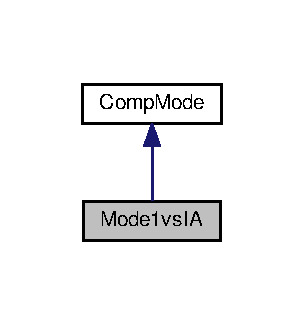
\includegraphics[width=146pt]{classMode1vsIA__inherit__graph}
\end{center}
\end{figure}


Collaboration diagram for Mode1vs\+I\+A\+:
\nopagebreak
\begin{figure}[H]
\begin{center}
\leavevmode
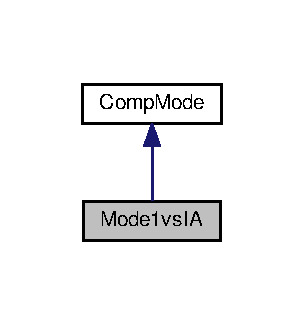
\includegraphics[width=146pt]{classMode1vsIA__coll__graph}
\end{center}
\end{figure}
\subsection*{Public Member Functions}
\begin{DoxyCompactItemize}
\item 
\hyperlink{classMode1vsIA_af8c73f16906279a89df6e9d150dfb1a2}{Mode1vs\+I\+A} ()
\begin{DoxyCompactList}\small\item\em Constructeur. \end{DoxyCompactList}\item 
void \hyperlink{classMode1vsIA_a8853a5c4bd43685f2232929f9d9d8732}{get\+Mode} ()
\begin{DoxyCompactList}\small\item\em Décrit le mode dans lequel on est. \end{DoxyCompactList}\item 
void \hyperlink{classMode1vsIA_a2e92031d0b7626da4f87ecc856a4ae94}{initialiser} ()
\begin{DoxyCompactList}\small\item\em Initialiser la carte d'initialisation. \end{DoxyCompactList}\item 
void \hyperlink{classMode1vsIA_ab6aa884defaf26231ede82d689b80d60}{lancer} ()
\begin{DoxyCompactList}\small\item\em Indiquer lorsque le J2 a fini d'initialiser sa carte. \end{DoxyCompactList}\item 
void \hyperlink{classMode1vsIA_ab50fb645a214d5cfab5fdb7a2b98673c}{fin\+Init\+J1} ()
\begin{DoxyCompactList}\small\item\em Indiquer lorsque le J1 a fini d'initialiser sa carte. \end{DoxyCompactList}\item 
void \hyperlink{classMode1vsIA_a7f7ab3fae5995ab12d6ce508c3d7dbca}{jouer} ()
\begin{DoxyCompactList}\small\item\em Jouer pour le mode 1\+V\+S\+I\+A. \end{DoxyCompactList}\item 
void \hyperlink{classMode1vsIA_a1da5810e6d744e2cbeae3ceebe6df521}{touche} ()
\begin{DoxyCompactList}\small\item\em Action produit après avoir touché un bateau. \end{DoxyCompactList}\item 
void \hyperlink{classMode1vsIA_a6c4e65dc4d95046165ce46b01cee6fad}{set\+Affichage} (std\+::shared\+\_\+ptr$<$ \hyperlink{classIAffichage}{I\+Affichage} $>$ aff)
\begin{DoxyCompactList}\small\item\em Permet de changer l'affichage actif. \end{DoxyCompactList}\item 
void \hyperlink{classMode1vsIA_a3dce01c56c0c5008f0e7a4dcb4d9834a}{choix\+Pour\+J2} ()
\begin{DoxyCompactList}\small\item\em Action produit pour le J2. \end{DoxyCompactList}\item 
\hypertarget{classMode1vsIA_a5dfd66257c3b315dda1a3d0a03670991}{virtual \hyperlink{classMode1vsIA_a5dfd66257c3b315dda1a3d0a03670991}{$\sim$\+Mode1vs\+I\+A} ()}\label{classMode1vsIA_a5dfd66257c3b315dda1a3d0a03670991}

\begin{DoxyCompactList}\small\item\em Destructeur Destructeur de la classe \hyperlink{classMode1vs1}{Mode1vs1}. \end{DoxyCompactList}\end{DoxyCompactItemize}
\subsection*{Additional Inherited Members}


\subsection{Detailed Description}
classe representant le mode de jeu 1\+V\+S\+I\+A 

La classe décrit les comportements pour le mode de jeu 1\+V\+S\+I\+A 

\subsection{Constructor \& Destructor Documentation}
\hypertarget{classMode1vsIA_af8c73f16906279a89df6e9d150dfb1a2}{\index{Mode1vs\+I\+A@{Mode1vs\+I\+A}!Mode1vs\+I\+A@{Mode1vs\+I\+A}}
\index{Mode1vs\+I\+A@{Mode1vs\+I\+A}!Mode1vs\+I\+A@{Mode1vs\+I\+A}}
\subsubsection[{Mode1vs\+I\+A}]{\setlength{\rightskip}{0pt plus 5cm}Mode1vs\+I\+A\+::\+Mode1vs\+I\+A (
\begin{DoxyParamCaption}
{}
\end{DoxyParamCaption}
)}}\label{classMode1vsIA_af8c73f16906279a89df6e9d150dfb1a2}


Constructeur. 

Constructeur de la classe \hyperlink{classMode1vsIA}{Mode1vs\+I\+A} 

\subsection{Member Function Documentation}
\hypertarget{classMode1vsIA_a3dce01c56c0c5008f0e7a4dcb4d9834a}{\index{Mode1vs\+I\+A@{Mode1vs\+I\+A}!choix\+Pour\+J2@{choix\+Pour\+J2}}
\index{choix\+Pour\+J2@{choix\+Pour\+J2}!Mode1vs\+I\+A@{Mode1vs\+I\+A}}
\subsubsection[{choix\+Pour\+J2}]{\setlength{\rightskip}{0pt plus 5cm}void Mode1vs\+I\+A\+::choix\+Pour\+J2 (
\begin{DoxyParamCaption}
{}
\end{DoxyParamCaption}
)\hspace{0.3cm}{\ttfamily [virtual]}}}\label{classMode1vsIA_a3dce01c56c0c5008f0e7a4dcb4d9834a}


Action produit pour le J2. 

Méthode permettant de choisir l'action à effectuer pour le J2 Pour ce mode, on initialise l'I\+A puis on lance le jeu 

Implements \hyperlink{classCompMode_a537f7077c642a62627ab008bc85642df}{Comp\+Mode}.

\hypertarget{classMode1vsIA_ab50fb645a214d5cfab5fdb7a2b98673c}{\index{Mode1vs\+I\+A@{Mode1vs\+I\+A}!fin\+Init\+J1@{fin\+Init\+J1}}
\index{fin\+Init\+J1@{fin\+Init\+J1}!Mode1vs\+I\+A@{Mode1vs\+I\+A}}
\subsubsection[{fin\+Init\+J1}]{\setlength{\rightskip}{0pt plus 5cm}void Mode1vs\+I\+A\+::fin\+Init\+J1 (
\begin{DoxyParamCaption}
{}
\end{DoxyParamCaption}
)\hspace{0.3cm}{\ttfamily [virtual]}}}\label{classMode1vsIA_ab50fb645a214d5cfab5fdb7a2b98673c}


Indiquer lorsque le J1 a fini d'initialiser sa carte. 

Méthode permettant de passer à la phase d'initialisation pour le J2 

Implements \hyperlink{classCompMode_a1e3c25af2e4e655d8ab55b77854069d7}{Comp\+Mode}.

\hypertarget{classMode1vsIA_a8853a5c4bd43685f2232929f9d9d8732}{\index{Mode1vs\+I\+A@{Mode1vs\+I\+A}!get\+Mode@{get\+Mode}}
\index{get\+Mode@{get\+Mode}!Mode1vs\+I\+A@{Mode1vs\+I\+A}}
\subsubsection[{get\+Mode}]{\setlength{\rightskip}{0pt plus 5cm}void Mode1vs\+I\+A\+::get\+Mode (
\begin{DoxyParamCaption}
{}
\end{DoxyParamCaption}
)\hspace{0.3cm}{\ttfamily [virtual]}}}\label{classMode1vsIA_a8853a5c4bd43685f2232929f9d9d8732}


Décrit le mode dans lequel on est. 

Méthode permettant décrire le mode 1\+V\+I\+A 

Implements \hyperlink{classCompMode_a897f6f474d86453c91ab83ab61c6f031}{Comp\+Mode}.

\hypertarget{classMode1vsIA_a2e92031d0b7626da4f87ecc856a4ae94}{\index{Mode1vs\+I\+A@{Mode1vs\+I\+A}!initialiser@{initialiser}}
\index{initialiser@{initialiser}!Mode1vs\+I\+A@{Mode1vs\+I\+A}}
\subsubsection[{initialiser}]{\setlength{\rightskip}{0pt plus 5cm}void Mode1vs\+I\+A\+::initialiser (
\begin{DoxyParamCaption}
{}
\end{DoxyParamCaption}
)\hspace{0.3cm}{\ttfamily [virtual]}}}\label{classMode1vsIA_a2e92031d0b7626da4f87ecc856a4ae94}


Initialiser la carte d'initialisation. 

Méthode permettant d'initialiser la carte Initialise de manière aléatoire les bateaux de l'I\+A 

Implements \hyperlink{classCompMode_a3559cd952b7f3c6f8e7f22f6f3dc23ae}{Comp\+Mode}.

\hypertarget{classMode1vsIA_a7f7ab3fae5995ab12d6ce508c3d7dbca}{\index{Mode1vs\+I\+A@{Mode1vs\+I\+A}!jouer@{jouer}}
\index{jouer@{jouer}!Mode1vs\+I\+A@{Mode1vs\+I\+A}}
\subsubsection[{jouer}]{\setlength{\rightskip}{0pt plus 5cm}void Mode1vs\+I\+A\+::jouer (
\begin{DoxyParamCaption}
{}
\end{DoxyParamCaption}
)\hspace{0.3cm}{\ttfamily [virtual]}}}\label{classMode1vsIA_a7f7ab3fae5995ab12d6ce508c3d7dbca}


Jouer pour le mode 1\+V\+S\+I\+A. 

Méthode permettant de décrire les actions produits pendant un tour de jeu On gère aussi lorsque l'I\+A touche des bateaux du J1 

Implements \hyperlink{classCompMode_a81615504b7d72e0255b7fc09a991e0b5}{Comp\+Mode}.

\hypertarget{classMode1vsIA_ab6aa884defaf26231ede82d689b80d60}{\index{Mode1vs\+I\+A@{Mode1vs\+I\+A}!lancer@{lancer}}
\index{lancer@{lancer}!Mode1vs\+I\+A@{Mode1vs\+I\+A}}
\subsubsection[{lancer}]{\setlength{\rightskip}{0pt plus 5cm}void Mode1vs\+I\+A\+::lancer (
\begin{DoxyParamCaption}
{}
\end{DoxyParamCaption}
)\hspace{0.3cm}{\ttfamily [virtual]}}}\label{classMode1vsIA_ab6aa884defaf26231ede82d689b80d60}


Indiquer lorsque le J2 a fini d'initialiser sa carte. 

Méthode permettant de passer à la phase de jeu 

Implements \hyperlink{classCompMode_a311cf95ec88795dfb14dbed569a7d54f}{Comp\+Mode}.

\hypertarget{classMode1vsIA_a6c4e65dc4d95046165ce46b01cee6fad}{\index{Mode1vs\+I\+A@{Mode1vs\+I\+A}!set\+Affichage@{set\+Affichage}}
\index{set\+Affichage@{set\+Affichage}!Mode1vs\+I\+A@{Mode1vs\+I\+A}}
\subsubsection[{set\+Affichage}]{\setlength{\rightskip}{0pt plus 5cm}void Mode1vs\+I\+A\+::set\+Affichage (
\begin{DoxyParamCaption}
\item[{std\+::shared\+\_\+ptr$<$ {\bf I\+Affichage} $>$}]{aff}
\end{DoxyParamCaption}
)\hspace{0.3cm}{\ttfamily [virtual]}}}\label{classMode1vsIA_a6c4e65dc4d95046165ce46b01cee6fad}


Permet de changer l'affichage actif. 

Méthode permettant changer l'affichage actif pour pouvoir effectuer les actions nécessaires 

Implements \hyperlink{classCompMode_a94119b30f5d6704464023e97b5656e9d}{Comp\+Mode}.

\hypertarget{classMode1vsIA_a1da5810e6d744e2cbeae3ceebe6df521}{\index{Mode1vs\+I\+A@{Mode1vs\+I\+A}!touche@{touche}}
\index{touche@{touche}!Mode1vs\+I\+A@{Mode1vs\+I\+A}}
\subsubsection[{touche}]{\setlength{\rightskip}{0pt plus 5cm}void Mode1vs\+I\+A\+::touche (
\begin{DoxyParamCaption}
{}
\end{DoxyParamCaption}
)\hspace{0.3cm}{\ttfamily [virtual]}}}\label{classMode1vsIA_a1da5810e6d744e2cbeae3ceebe6df521}


Action produit après avoir touché un bateau. 

Méthode permettant de décrire les actions à faire après avoir touché un bateau de l'I\+A 

Implements \hyperlink{classCompMode_a6b26d4c754fe0cc104d24d79f472b24d}{Comp\+Mode}.



The documentation for this class was generated from the following files\+:\begin{DoxyCompactItemize}
\item 
mode1vsia.\+h\item 
mode1vsia.\+cpp\end{DoxyCompactItemize}

\hypertarget{classOie}{\section{Oie Class Reference}
\label{classOie}\index{Oie@{Oie}}
}


classe representant un \hyperlink{classOie}{Oie}  




{\ttfamily \#include $<$oie.\+h$>$}



Inheritance diagram for Oie\+:
\nopagebreak
\begin{figure}[H]
\begin{center}
\leavevmode
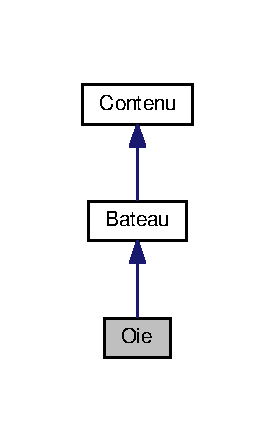
\includegraphics[width=132pt]{classOie__inherit__graph}
\end{center}
\end{figure}


Collaboration diagram for Oie\+:
\nopagebreak
\begin{figure}[H]
\begin{center}
\leavevmode
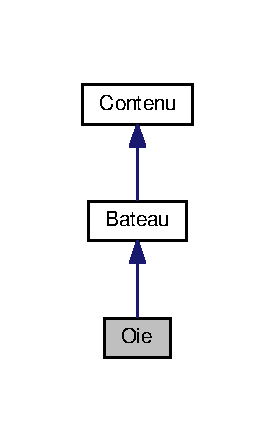
\includegraphics[width=132pt]{classOie__coll__graph}
\end{center}
\end{figure}
\subsection*{Public Member Functions}
\begin{DoxyCompactItemize}
\item 
\hyperlink{classOie_a0d6e4a1f091635c9292f2805fbb1f76f}{Oie} ()
\begin{DoxyCompactList}\small\item\em Constructeur. \end{DoxyCompactList}\item 
int \hyperlink{classOie_aa07fdf5abd6eec1a4578a90edb029ad1}{get\+Taille} ()
\begin{DoxyCompactList}\small\item\em Récupère la taille du \hyperlink{classBateau}{Bateau}. \end{DoxyCompactList}\end{DoxyCompactItemize}
\subsection*{Additional Inherited Members}


\subsection{Detailed Description}
classe representant un \hyperlink{classOie}{Oie} 

La classe modélise un \hyperlink{classBateau}{Bateau} de taille 3 

\subsection{Constructor \& Destructor Documentation}
\hypertarget{classOie_a0d6e4a1f091635c9292f2805fbb1f76f}{\index{Oie@{Oie}!Oie@{Oie}}
\index{Oie@{Oie}!Oie@{Oie}}
\subsubsection[{Oie}]{\setlength{\rightskip}{0pt plus 5cm}Oie\+::\+Oie (
\begin{DoxyParamCaption}
{}
\end{DoxyParamCaption}
)}}\label{classOie_a0d6e4a1f091635c9292f2805fbb1f76f}


Constructeur. 

Constructeur de la classe \hyperlink{classOie}{Oie} 

\subsection{Member Function Documentation}
\hypertarget{classOie_aa07fdf5abd6eec1a4578a90edb029ad1}{\index{Oie@{Oie}!get\+Taille@{get\+Taille}}
\index{get\+Taille@{get\+Taille}!Oie@{Oie}}
\subsubsection[{get\+Taille}]{\setlength{\rightskip}{0pt plus 5cm}int Oie\+::get\+Taille (
\begin{DoxyParamCaption}
{}
\end{DoxyParamCaption}
)\hspace{0.3cm}{\ttfamily [virtual]}}}\label{classOie_aa07fdf5abd6eec1a4578a90edb029ad1}


Récupère la taille du \hyperlink{classBateau}{Bateau}. 

Méthode permettant de récupérer la taille d'une \hyperlink{classOie}{Oie}

\begin{DoxyReturn}{Returns}
la taille d'une \hyperlink{classOie}{Oie} (3) 
\end{DoxyReturn}


Implements \hyperlink{classBateau_a08be20b8c871149d717a30b00c1068b9}{Bateau}.



The documentation for this class was generated from the following files\+:\begin{DoxyCompactItemize}
\item 
oie.\+h\item 
oie.\+cpp\end{DoxyCompactItemize}

\hypertarget{structqt__meta__stringdata__AffichageInitJ1__t}{\section{qt\+\_\+meta\+\_\+stringdata\+\_\+\+Affichage\+Init\+J1\+\_\+t Struct Reference}
\label{structqt__meta__stringdata__AffichageInitJ1__t}\index{qt\+\_\+meta\+\_\+stringdata\+\_\+\+Affichage\+Init\+J1\+\_\+t@{qt\+\_\+meta\+\_\+stringdata\+\_\+\+Affichage\+Init\+J1\+\_\+t}}
}
\subsection*{Public Attributes}
\begin{DoxyCompactItemize}
\item 
\hypertarget{structqt__meta__stringdata__AffichageInitJ1__t_a6e4f85ed6b8fd34fcafe5c9a3e649986}{Q\+Byte\+Array\+Data {\bfseries data} \mbox{[}4\mbox{]}}\label{structqt__meta__stringdata__AffichageInitJ1__t_a6e4f85ed6b8fd34fcafe5c9a3e649986}

\item 
\hypertarget{structqt__meta__stringdata__AffichageInitJ1__t_a3ba448ce151e74e7c98f58315a2724c2}{char {\bfseries stringdata} \mbox{[}44\mbox{]}}\label{structqt__meta__stringdata__AffichageInitJ1__t_a3ba448ce151e74e7c98f58315a2724c2}

\end{DoxyCompactItemize}


The documentation for this struct was generated from the following file\+:\begin{DoxyCompactItemize}
\item 
moc\+\_\+affichageinitj1.\+cpp\end{DoxyCompactItemize}

\hypertarget{structqt__meta__stringdata__AffichageInitJ2__t}{\section{qt\+\_\+meta\+\_\+stringdata\+\_\+\+Affichage\+Init\+J2\+\_\+t Struct Reference}
\label{structqt__meta__stringdata__AffichageInitJ2__t}\index{qt\+\_\+meta\+\_\+stringdata\+\_\+\+Affichage\+Init\+J2\+\_\+t@{qt\+\_\+meta\+\_\+stringdata\+\_\+\+Affichage\+Init\+J2\+\_\+t}}
}
\subsection*{Public Attributes}
\begin{DoxyCompactItemize}
\item 
\hypertarget{structqt__meta__stringdata__AffichageInitJ2__t_a1cdbc0adf6fb95ef483de4d8ddd83d72}{Q\+Byte\+Array\+Data {\bfseries data} \mbox{[}4\mbox{]}}\label{structqt__meta__stringdata__AffichageInitJ2__t_a1cdbc0adf6fb95ef483de4d8ddd83d72}

\item 
\hypertarget{structqt__meta__stringdata__AffichageInitJ2__t_ae3684bd8160bd567b5461ced5212a46a}{char {\bfseries stringdata} \mbox{[}44\mbox{]}}\label{structqt__meta__stringdata__AffichageInitJ2__t_ae3684bd8160bd567b5461ced5212a46a}

\end{DoxyCompactItemize}


The documentation for this struct was generated from the following file\+:\begin{DoxyCompactItemize}
\item 
moc\+\_\+affichageinitj2.\+cpp\end{DoxyCompactItemize}

\hypertarget{structqt__meta__stringdata__AffichageJeu__t}{\section{qt\+\_\+meta\+\_\+stringdata\+\_\+\+Affichage\+Jeu\+\_\+t Struct Reference}
\label{structqt__meta__stringdata__AffichageJeu__t}\index{qt\+\_\+meta\+\_\+stringdata\+\_\+\+Affichage\+Jeu\+\_\+t@{qt\+\_\+meta\+\_\+stringdata\+\_\+\+Affichage\+Jeu\+\_\+t}}
}
\subsection*{Public Attributes}
\begin{DoxyCompactItemize}
\item 
\hypertarget{structqt__meta__stringdata__AffichageJeu__t_a9e6727643de2550395b112dbca6f53fb}{Q\+Byte\+Array\+Data {\bfseries data} \mbox{[}1\mbox{]}}\label{structqt__meta__stringdata__AffichageJeu__t_a9e6727643de2550395b112dbca6f53fb}

\item 
\hypertarget{structqt__meta__stringdata__AffichageJeu__t_a4a947fe89aebb3bf8da241189c3efd48}{char {\bfseries stringdata} \mbox{[}14\mbox{]}}\label{structqt__meta__stringdata__AffichageJeu__t_a4a947fe89aebb3bf8da241189c3efd48}

\end{DoxyCompactItemize}


The documentation for this struct was generated from the following file\+:\begin{DoxyCompactItemize}
\item 
moc\+\_\+affichagejeu.\+cpp\end{DoxyCompactItemize}

\hypertarget{structqt__meta__stringdata__AffichageMenu__t}{\section{qt\+\_\+meta\+\_\+stringdata\+\_\+\+Affichage\+Menu\+\_\+t Struct Reference}
\label{structqt__meta__stringdata__AffichageMenu__t}\index{qt\+\_\+meta\+\_\+stringdata\+\_\+\+Affichage\+Menu\+\_\+t@{qt\+\_\+meta\+\_\+stringdata\+\_\+\+Affichage\+Menu\+\_\+t}}
}
\subsection*{Public Attributes}
\begin{DoxyCompactItemize}
\item 
\hypertarget{structqt__meta__stringdata__AffichageMenu__t_a00a509271c61838a0f782068da0f0dc9}{Q\+Byte\+Array\+Data {\bfseries data} \mbox{[}4\mbox{]}}\label{structqt__meta__stringdata__AffichageMenu__t_a00a509271c61838a0f782068da0f0dc9}

\item 
\hypertarget{structqt__meta__stringdata__AffichageMenu__t_a040ab3479a5309eadb0e8073af2fdaac}{char {\bfseries stringdata} \mbox{[}43\mbox{]}}\label{structqt__meta__stringdata__AffichageMenu__t_a040ab3479a5309eadb0e8073af2fdaac}

\end{DoxyCompactItemize}


The documentation for this struct was generated from the following file\+:\begin{DoxyCompactItemize}
\item 
moc\+\_\+affichagemenu.\+cpp\end{DoxyCompactItemize}

\hypertarget{structqt__meta__stringdata__Carte__t}{\section{qt\+\_\+meta\+\_\+stringdata\+\_\+\+Carte\+\_\+t Struct Reference}
\label{structqt__meta__stringdata__Carte__t}\index{qt\+\_\+meta\+\_\+stringdata\+\_\+\+Carte\+\_\+t@{qt\+\_\+meta\+\_\+stringdata\+\_\+\+Carte\+\_\+t}}
}
\subsection*{Public Attributes}
\begin{DoxyCompactItemize}
\item 
\hypertarget{structqt__meta__stringdata__Carte__t_af14d5110e51b96e8db238f59dbe42704}{Q\+Byte\+Array\+Data {\bfseries data} \mbox{[}3\mbox{]}}\label{structqt__meta__stringdata__Carte__t_af14d5110e51b96e8db238f59dbe42704}

\item 
\hypertarget{structqt__meta__stringdata__Carte__t_ab444d03dcb9c21da9cb263531278c892}{char {\bfseries stringdata} \mbox{[}21\mbox{]}}\label{structqt__meta__stringdata__Carte__t_ab444d03dcb9c21da9cb263531278c892}

\end{DoxyCompactItemize}


The documentation for this struct was generated from the following file\+:\begin{DoxyCompactItemize}
\item 
moc\+\_\+carte.\+cpp\end{DoxyCompactItemize}

\hypertarget{structqt__meta__stringdata__Case__t}{\section{qt\+\_\+meta\+\_\+stringdata\+\_\+\+Case\+\_\+t Struct Reference}
\label{structqt__meta__stringdata__Case__t}\index{qt\+\_\+meta\+\_\+stringdata\+\_\+\+Case\+\_\+t@{qt\+\_\+meta\+\_\+stringdata\+\_\+\+Case\+\_\+t}}
}
\subsection*{Public Attributes}
\begin{DoxyCompactItemize}
\item 
\hypertarget{structqt__meta__stringdata__Case__t_a6f3a1b9b3e1fac94a6b966e7074dc7d9}{Q\+Byte\+Array\+Data {\bfseries data} \mbox{[}1\mbox{]}}\label{structqt__meta__stringdata__Case__t_a6f3a1b9b3e1fac94a6b966e7074dc7d9}

\item 
\hypertarget{structqt__meta__stringdata__Case__t_afd1a2b5ae2084283aa5cea8842791b41}{char {\bfseries stringdata} \mbox{[}6\mbox{]}}\label{structqt__meta__stringdata__Case__t_afd1a2b5ae2084283aa5cea8842791b41}

\end{DoxyCompactItemize}


The documentation for this struct was generated from the following file\+:\begin{DoxyCompactItemize}
\item 
moc\+\_\+case.\+cpp\end{DoxyCompactItemize}

\hypertarget{structqt__meta__stringdata__IAffichage__t}{\section{qt\+\_\+meta\+\_\+stringdata\+\_\+\+I\+Affichage\+\_\+t Struct Reference}
\label{structqt__meta__stringdata__IAffichage__t}\index{qt\+\_\+meta\+\_\+stringdata\+\_\+\+I\+Affichage\+\_\+t@{qt\+\_\+meta\+\_\+stringdata\+\_\+\+I\+Affichage\+\_\+t}}
}
\subsection*{Public Attributes}
\begin{DoxyCompactItemize}
\item 
\hypertarget{structqt__meta__stringdata__IAffichage__t_a657597828cc58e47411787993af24b1f}{Q\+Byte\+Array\+Data {\bfseries data} \mbox{[}1\mbox{]}}\label{structqt__meta__stringdata__IAffichage__t_a657597828cc58e47411787993af24b1f}

\item 
\hypertarget{structqt__meta__stringdata__IAffichage__t_a2c0d8bb42829e61fe97cb8e399594d28}{char {\bfseries stringdata} \mbox{[}12\mbox{]}}\label{structqt__meta__stringdata__IAffichage__t_a2c0d8bb42829e61fe97cb8e399594d28}

\end{DoxyCompactItemize}


The documentation for this struct was generated from the following file\+:\begin{DoxyCompactItemize}
\item 
moc\+\_\+iaffichage.\+cpp\end{DoxyCompactItemize}

\hypertarget{classTeam}{\section{Team Class Reference}
\label{classTeam}\index{Team@{Team}}
}


classe representant un Joueur  




{\ttfamily \#include $<$team.\+h$>$}

\subsection*{Public Member Functions}
\begin{DoxyCompactItemize}
\item 
\hyperlink{classTeam_aada295895b747960576b69d8c87a54ba}{Team} ()
\begin{DoxyCompactList}\small\item\em Constructeur. \end{DoxyCompactList}\item 
std\+::shared\+\_\+ptr$<$ \hyperlink{classCarte}{Carte} $>$ \hyperlink{classTeam_a8437fa1637e3a4669a676035e9d2fa56}{get\+Carte\+Init} ()
\begin{DoxyCompactList}\small\item\em Récupère la carte d'initialisation du Joueur. \end{DoxyCompactList}\item 
void \hyperlink{classTeam_a3af475d5b149db7883694bed764ddf04}{set\+Carte\+Init} (std\+::shared\+\_\+ptr$<$ \hyperlink{classCarte}{Carte} $>$ c)
\begin{DoxyCompactList}\small\item\em Modifie la carte d'initialisation. \end{DoxyCompactList}\item 
std\+::shared\+\_\+ptr$<$ \hyperlink{classCarte}{Carte} $>$ \hyperlink{classTeam_a25cc34febbd1876085272a62ce96fb2c}{get\+Carte\+Jeu} ()
\begin{DoxyCompactList}\small\item\em Récupère la carte de jeu du Joueur. \end{DoxyCompactList}\item 
void \hyperlink{classTeam_a0786a89ae3fd8fc20d327ddd3e07b2cf}{set\+Carte\+Jeu} (std\+::shared\+\_\+ptr$<$ \hyperlink{classCarte}{Carte} $>$ c)
\begin{DoxyCompactList}\small\item\em Modifie la carte de jeu. \end{DoxyCompactList}\item 
std\+::string \hyperlink{classTeam_a7bba8af6230814d10edb9312dd13069b}{get\+Pseudo} ()
\begin{DoxyCompactList}\small\item\em Récupère le pseudo du Joueur. \end{DoxyCompactList}\item 
void \hyperlink{classTeam_a21cb86bba554a00f774ed417336f3957}{set\+Pseudo} (std\+::string p)
\begin{DoxyCompactList}\small\item\em Modifie le pseudo du Joueur. \end{DoxyCompactList}\item 
bool \hyperlink{classTeam_a71301541074a696ce146c89c2c399093}{get\+Is\+Turn} ()
\begin{DoxyCompactList}\small\item\em Savoir à qui est le tour de jeu. \end{DoxyCompactList}\item 
void \hyperlink{classTeam_a0bb7e1d431a4d343a9c694c04f967706}{set\+Is\+Turn} (bool t)
\begin{DoxyCompactList}\small\item\em Modifie le tour du Joueur. \end{DoxyCompactList}\end{DoxyCompactItemize}


\subsection{Detailed Description}
classe representant un Joueur 

La classe modélise un Joueur et ce qui le compose 

\subsection{Constructor \& Destructor Documentation}
\hypertarget{classTeam_aada295895b747960576b69d8c87a54ba}{\index{Team@{Team}!Team@{Team}}
\index{Team@{Team}!Team@{Team}}
\subsubsection[{Team}]{\setlength{\rightskip}{0pt plus 5cm}Team\+::\+Team (
\begin{DoxyParamCaption}
{}
\end{DoxyParamCaption}
)}}\label{classTeam_aada295895b747960576b69d8c87a54ba}


Constructeur. 

Constructeur de la classe \hyperlink{classTeam}{Team} 

\subsection{Member Function Documentation}
\hypertarget{classTeam_a8437fa1637e3a4669a676035e9d2fa56}{\index{Team@{Team}!get\+Carte\+Init@{get\+Carte\+Init}}
\index{get\+Carte\+Init@{get\+Carte\+Init}!Team@{Team}}
\subsubsection[{get\+Carte\+Init}]{\setlength{\rightskip}{0pt plus 5cm}shared\+\_\+ptr$<$ {\bf Carte} $>$ Team\+::get\+Carte\+Init (
\begin{DoxyParamCaption}
{}
\end{DoxyParamCaption}
)}}\label{classTeam_a8437fa1637e3a4669a676035e9d2fa56}


Récupère la carte d'initialisation du Joueur. 

Méthode permettant de récupérer la carte d'initialisation du joueur une fois qu'il a fini

\begin{DoxyReturn}{Returns}
la carte d'initialisation 
\end{DoxyReturn}
\hypertarget{classTeam_a25cc34febbd1876085272a62ce96fb2c}{\index{Team@{Team}!get\+Carte\+Jeu@{get\+Carte\+Jeu}}
\index{get\+Carte\+Jeu@{get\+Carte\+Jeu}!Team@{Team}}
\subsubsection[{get\+Carte\+Jeu}]{\setlength{\rightskip}{0pt plus 5cm}shared\+\_\+ptr$<$ {\bf Carte} $>$ Team\+::get\+Carte\+Jeu (
\begin{DoxyParamCaption}
{}
\end{DoxyParamCaption}
)}}\label{classTeam_a25cc34febbd1876085272a62ce96fb2c}


Récupère la carte de jeu du Joueur. 

Méthode permettant de récupérer la carte de jeu

\begin{DoxyReturn}{Returns}
la carte de jeu du Joueur 
\end{DoxyReturn}
\hypertarget{classTeam_a71301541074a696ce146c89c2c399093}{\index{Team@{Team}!get\+Is\+Turn@{get\+Is\+Turn}}
\index{get\+Is\+Turn@{get\+Is\+Turn}!Team@{Team}}
\subsubsection[{get\+Is\+Turn}]{\setlength{\rightskip}{0pt plus 5cm}bool Team\+::get\+Is\+Turn (
\begin{DoxyParamCaption}
{}
\end{DoxyParamCaption}
)}}\label{classTeam_a71301541074a696ce146c89c2c399093}


Savoir à qui est le tour de jeu. 

Méthode permettant de savoir si c'est au tour du Joueur 1 ou du Joueur 2

\begin{DoxyReturn}{Returns}
si c'est au tour du Joueur courant 
\end{DoxyReturn}
\hypertarget{classTeam_a7bba8af6230814d10edb9312dd13069b}{\index{Team@{Team}!get\+Pseudo@{get\+Pseudo}}
\index{get\+Pseudo@{get\+Pseudo}!Team@{Team}}
\subsubsection[{get\+Pseudo}]{\setlength{\rightskip}{0pt plus 5cm}string Team\+::get\+Pseudo (
\begin{DoxyParamCaption}
{}
\end{DoxyParamCaption}
)}}\label{classTeam_a7bba8af6230814d10edb9312dd13069b}


Récupère le pseudo du Joueur. 

Méthode permettant de récupérer le pseudo du joueur

\begin{DoxyReturn}{Returns}
le pseudo du Joueur 
\end{DoxyReturn}
\hypertarget{classTeam_a3af475d5b149db7883694bed764ddf04}{\index{Team@{Team}!set\+Carte\+Init@{set\+Carte\+Init}}
\index{set\+Carte\+Init@{set\+Carte\+Init}!Team@{Team}}
\subsubsection[{set\+Carte\+Init}]{\setlength{\rightskip}{0pt plus 5cm}void Team\+::set\+Carte\+Init (
\begin{DoxyParamCaption}
\item[{std\+::shared\+\_\+ptr$<$ {\bf Carte} $>$}]{c}
\end{DoxyParamCaption}
)}}\label{classTeam_a3af475d5b149db7883694bed764ddf04}


Modifie la carte d'initialisation. 

Méthode permettant de modifier la carte d'initialisation après l'ajout des bateaux


\begin{DoxyParams}{Parameters}
{\em c} & \+: la carte d'initialisation \\
\hline
\end{DoxyParams}
\hypertarget{classTeam_a0786a89ae3fd8fc20d327ddd3e07b2cf}{\index{Team@{Team}!set\+Carte\+Jeu@{set\+Carte\+Jeu}}
\index{set\+Carte\+Jeu@{set\+Carte\+Jeu}!Team@{Team}}
\subsubsection[{set\+Carte\+Jeu}]{\setlength{\rightskip}{0pt plus 5cm}void Team\+::set\+Carte\+Jeu (
\begin{DoxyParamCaption}
\item[{std\+::shared\+\_\+ptr$<$ {\bf Carte} $>$}]{c}
\end{DoxyParamCaption}
)}}\label{classTeam_a0786a89ae3fd8fc20d327ddd3e07b2cf}


Modifie la carte de jeu. 

Méthode permettant de modifier la carte de jeu


\begin{DoxyParams}{Parameters}
{\em c} & \+: la carte de jeu \\
\hline
\end{DoxyParams}
\hypertarget{classTeam_a0bb7e1d431a4d343a9c694c04f967706}{\index{Team@{Team}!set\+Is\+Turn@{set\+Is\+Turn}}
\index{set\+Is\+Turn@{set\+Is\+Turn}!Team@{Team}}
\subsubsection[{set\+Is\+Turn}]{\setlength{\rightskip}{0pt plus 5cm}void Team\+::set\+Is\+Turn (
\begin{DoxyParamCaption}
\item[{bool}]{t}
\end{DoxyParamCaption}
)}}\label{classTeam_a0bb7e1d431a4d343a9c694c04f967706}


Modifie le tour du Joueur. 

Méthode permettant de modifier le tour du joueur courant


\begin{DoxyParams}{Parameters}
{\em t} & \+: booléen à true pour changer le tour, false sinon \\
\hline
\end{DoxyParams}
\hypertarget{classTeam_a21cb86bba554a00f774ed417336f3957}{\index{Team@{Team}!set\+Pseudo@{set\+Pseudo}}
\index{set\+Pseudo@{set\+Pseudo}!Team@{Team}}
\subsubsection[{set\+Pseudo}]{\setlength{\rightskip}{0pt plus 5cm}void Team\+::set\+Pseudo (
\begin{DoxyParamCaption}
\item[{std\+::string}]{p}
\end{DoxyParamCaption}
)}}\label{classTeam_a21cb86bba554a00f774ed417336f3957}


Modifie le pseudo du Joueur. 

Méthode permettant de modifier le pseudo du joueur


\begin{DoxyParams}{Parameters}
{\em p} & \+: le nouveau pseudo du joueur \\
\hline
\end{DoxyParams}


The documentation for this class was generated from the following files\+:\begin{DoxyCompactItemize}
\item 
team.\+h\item 
team.\+cpp\end{DoxyCompactItemize}

%--- End generated contents ---

% Index
\newpage
\phantomsection
\addcontentsline{toc}{chapter}{Index}
\printindex

\end{document}
